\documentclass[xcolor=pdftex,dvipsnames,table,mathserif]{beamer}
%\usepackage{subfigure}
\usepackage{amsbsy}
\usepackage{tikz}
\usetikzlibrary{arrows}
\usepackage{amsmath,graphicx,dsfont,color}
\usepackage{amsfonts}
\usepackage{amssymb}
\usepackage{array}

\usepackage{subfig}

% makes the subfig package work
\makeatletter
\let\@@magyar@captionfix\relax
\makeatother

% subfigure counter resets every frame
\makeatletter
\@addtoreset{subfigure}{framenumber}
\makeatother

% First author and year
\bibliographystyle{apalike}

% This sets the list items of the bibliography to the same symbol used for citation.
\setbeamertemplate{bibliography item}{\insertbiblabel}

% This avoids extralines for different entries
\setbeamertemplate{bibliography entry title}{}
\setbeamertemplate{bibliography entry location}{}
\setbeamertemplate{bibliography entry note}{}

\DeclareMathOperator*{\argmin}{arg\,min}
\DeclareMathOperator*{\argmax}{arg\,max}
%Definitiona

\newcommand{\x}{\mathbf{x}}
\newcommand{\X}{\mathbf{X}}
\newcommand{\W}{\mathbf{W}} %Weight
\newcommand{\bais}{\mathbf{b}}%Bais
\newcommand{\act}{\texttt{g}}%Activation
\newcommand{\loss}{L}
\newcommand{\pdata}{\hat{p}_{\texttt{data}}}
\newcommand{\nsize}{N}
\newcommand{\nfeatures}{P}
\newcommand{\param}{\boldsymbol{\theta}}
\newcommand{\featmap}{\boldsymbol{\phi}}
\newcommand{\EV}{\mathbb{E}}







\usepackage{physics}
\usepackage{tikz}
\usetikzlibrary{fit,positioning}

\graphicspath{{../graphics/}}

\AtBeginSection[]{
  \begin{frame}{Contents}
    \tableofcontents[currentsection, hideothersubsections]
  \end{frame}
}

\AtBeginSubsection[]{
  \begin{frame}{Contents}
    \tableofcontents[currentsection, subsectionstyle=show/shaded/hide]
  \end{frame}
}

\setbeamertemplate{footline}[frame number]{}
\setbeamertemplate{navigation symbols}{}
\setbeamertemplate{section in toc}[square]
\setbeamertemplate{items}[square]

%% For image credits on image bottom right
\usepackage[absolute,overlay]{textpos}
\setbeamercolor{framesource}{fg=gray}
\setbeamerfont{framesource}{size=\tiny}
\newcommand{\source}[1]{\begin{textblock*}{4cm}(8.7cm,8.6cm)
    \begin{beamercolorbox}[ht=0.5cm,right]{framesource}
      \usebeamerfont{framesource}\usebeamercolor[fg]{framesource} Credits: {#1}
    \end{beamercolorbox}
\end{textblock*}}

\title{Achievements and challenges of semantic image segmentation with deep learning}
\author{E. Decencière}
\date{MINES ParisTech\\
  PSL Research University\\
  Center for Mathematical Morphology
}
\titlegraphic{
\includegraphics[height=1.7cm]{../graphics/logoemp}}

\useinnertheme{rounded}
\usecolortheme{rose}

%%%%%%%%%%%%%%%%%%%%%%%%%%%%%%%%%%%%%%%%%%%%%%%%%%%%%%%
%%%%%%%%%%%%%%%%%%%%%%%%%%%%%%%%%%%%%%%%%%%%%%%%%%%%%%%

\begin{document}

\frame{\titlepage}

\frame{
  \frametitle{Contents}
  \tableofcontents[hidesubsections]
}

%%%%%%%%%%%%%%%%%%%%%%%%%%%%%%%%%%%%%%%%%%%%%%%%%%
%%%%%%%%%%%%%%%%%%%%%%%%%%%%%%%%%%%%%%%%%%%%%%%%%%
\section{Introduction}

%%%%%%%%%%%%%%%%%%%%%%%%%%%%%%%%%%%%
\begin{frame}{What is deep learning?}

\begin{block}{Definition}
    Deep learning is the branch of machine learning that studies artificial neural networks.
\end{block}

  \begin{block}{}
  \centering
    Deep Learning $\subset$ Machine Learning $\subset$ Artificial Intelligence
  \end{block}



\end{frame}


%%%%%%%%%%%%%%%%%%%%%%%%%%%%%%%%%%%%
\begin{frame}{A revolution in image analysis}

\begin{itemize}
\item 2010: graph cuts, snakes, mathematical morphology, machine learning, etc.
\item Today: deep learning.
\end{itemize}

\end{frame}


%%%%%%%%%%%%%%%%%%%%%%%%%%%%%%%%%%%%
\begin{frame}{The rise of deep learning}

\begin{figure}[ht]
  \centering
  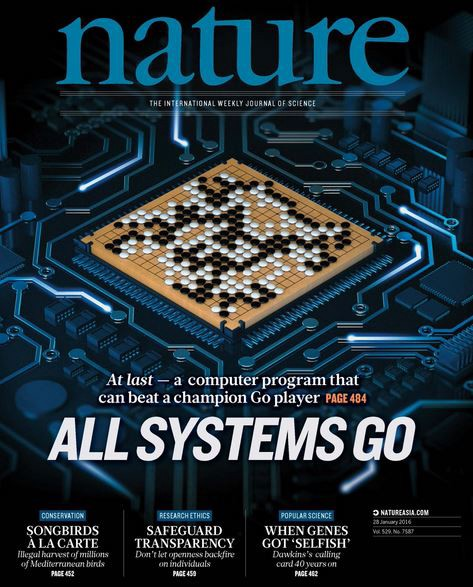
\includegraphics[height=0.5\textheight]{nature_go}
  \caption*{Nature, 2016}
\end{figure}


\end{frame}


%%%%%%%%%%%%%%%%%%%%%%%%%%%%%%%%%%%%
\begin{frame}{Differentiable programming}

\begin{block}{Definition}
  Differentiable programming is an algorithmic framework where differentiable operators are combined together to build complex systems. The parameters of the system can then be optimized via gradient descent thanks to \alert{back-propagation}.
\end{block}

The object of study of differential programming are \emph{computational graphs}.

\end{frame}
%%%%%%%%%%%%%%%%%%%%%%%%%%%%%%%%%%%%
\begin{frame}{Computational graph}

\begin{block}{Definition}
  A computational graph is a direct acyclic graph such that:
  \begin{itemize}
  \item A node is a mathematical operator
  \item To each edge is associated a value (scalar, vector, matrix, tensor, $\ldots$)
  \item Each node can compute the values of its output edges from the values of its input edges
  \end{itemize}
\end{block}

Computing a \emph{forward pass} through the graph means choosing its input values, and then progressively computing the values of all edges.


\end{frame}


%%%%%%%%%%%%%%%%%%%%%%%%%%%%%%%%%%%%
\begin{frame}{Computational graph example}
  Computational graph of:
  \[
  \sigma(w_1x + w_2y + b)
  \]
  where $\sigma$ is the sigmoid function: $\sigma(x) = \frac{1}{1 + e^{-x}}$

\vspace{3em}
\pause

  \centering
  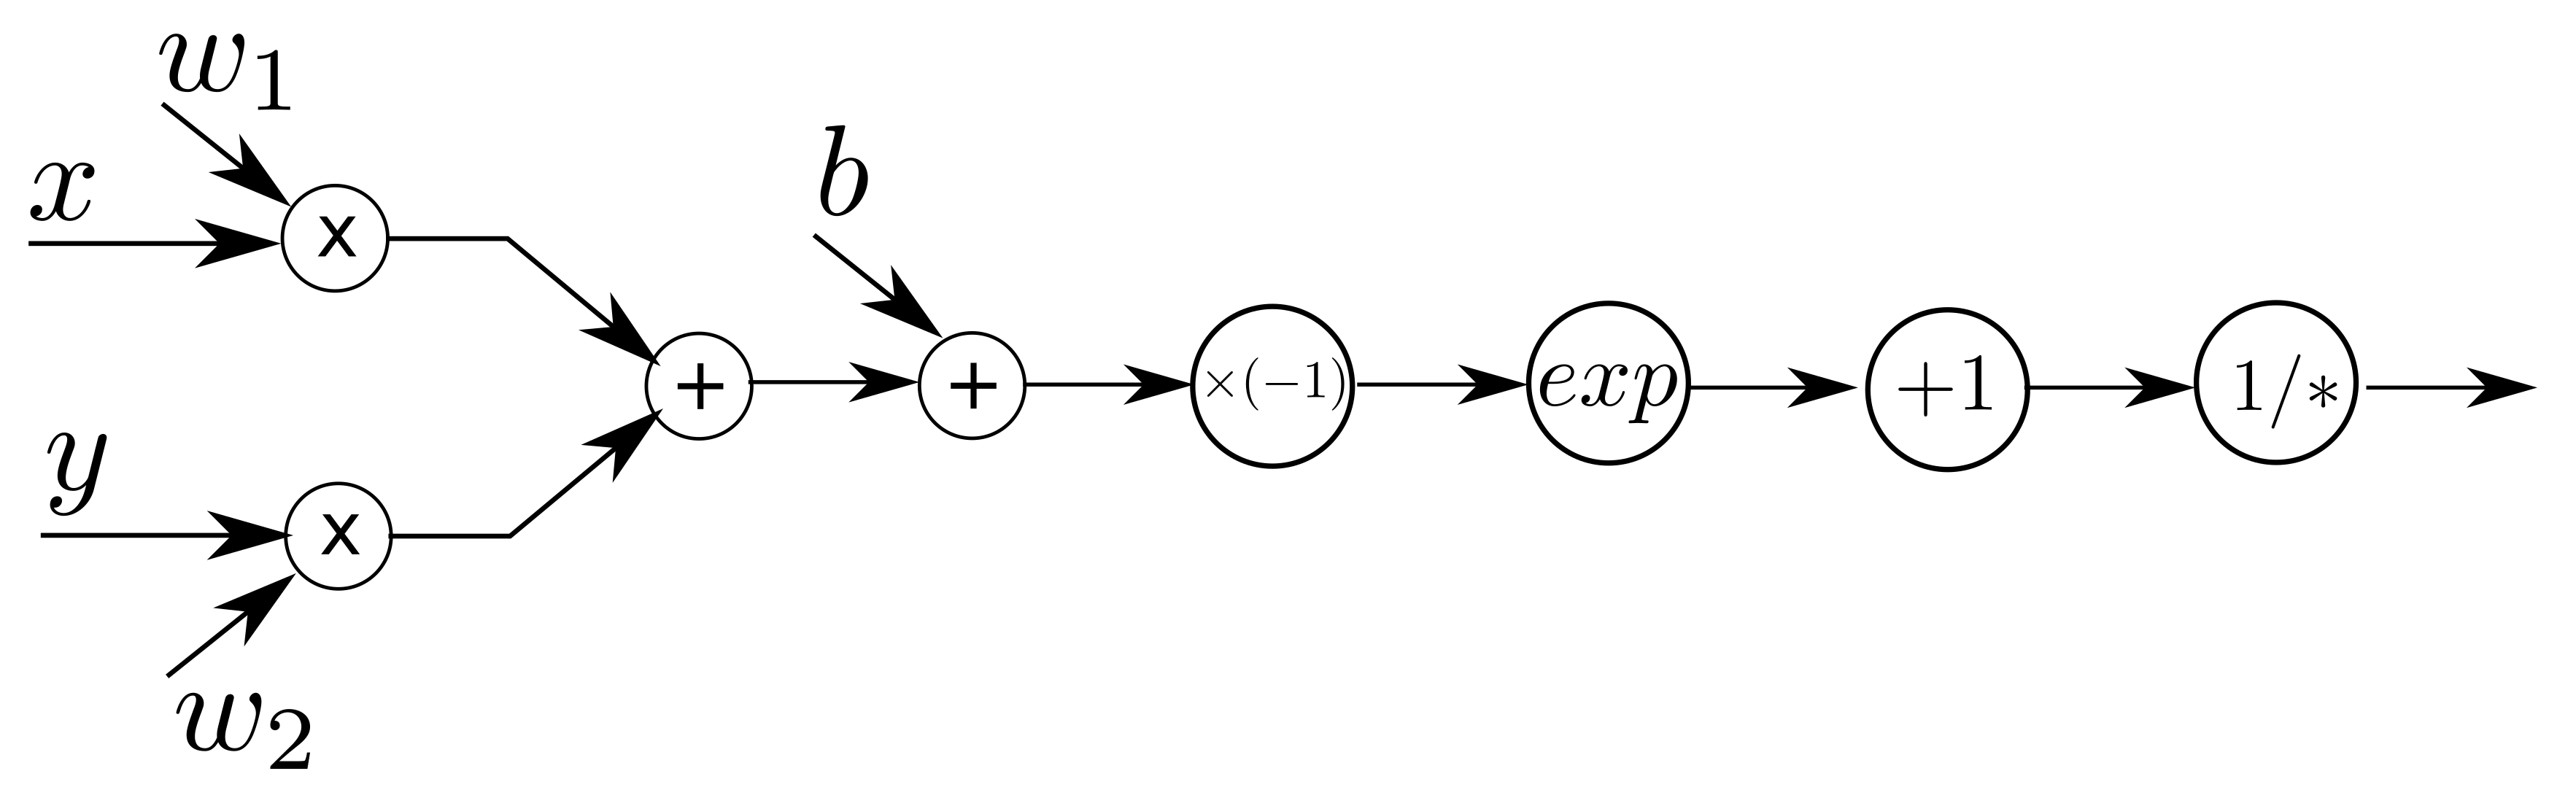
\includegraphics[width=0.7\textwidth]{comp_graph2}\\
  \pause
  The graph can be represented at different levels of detail:
  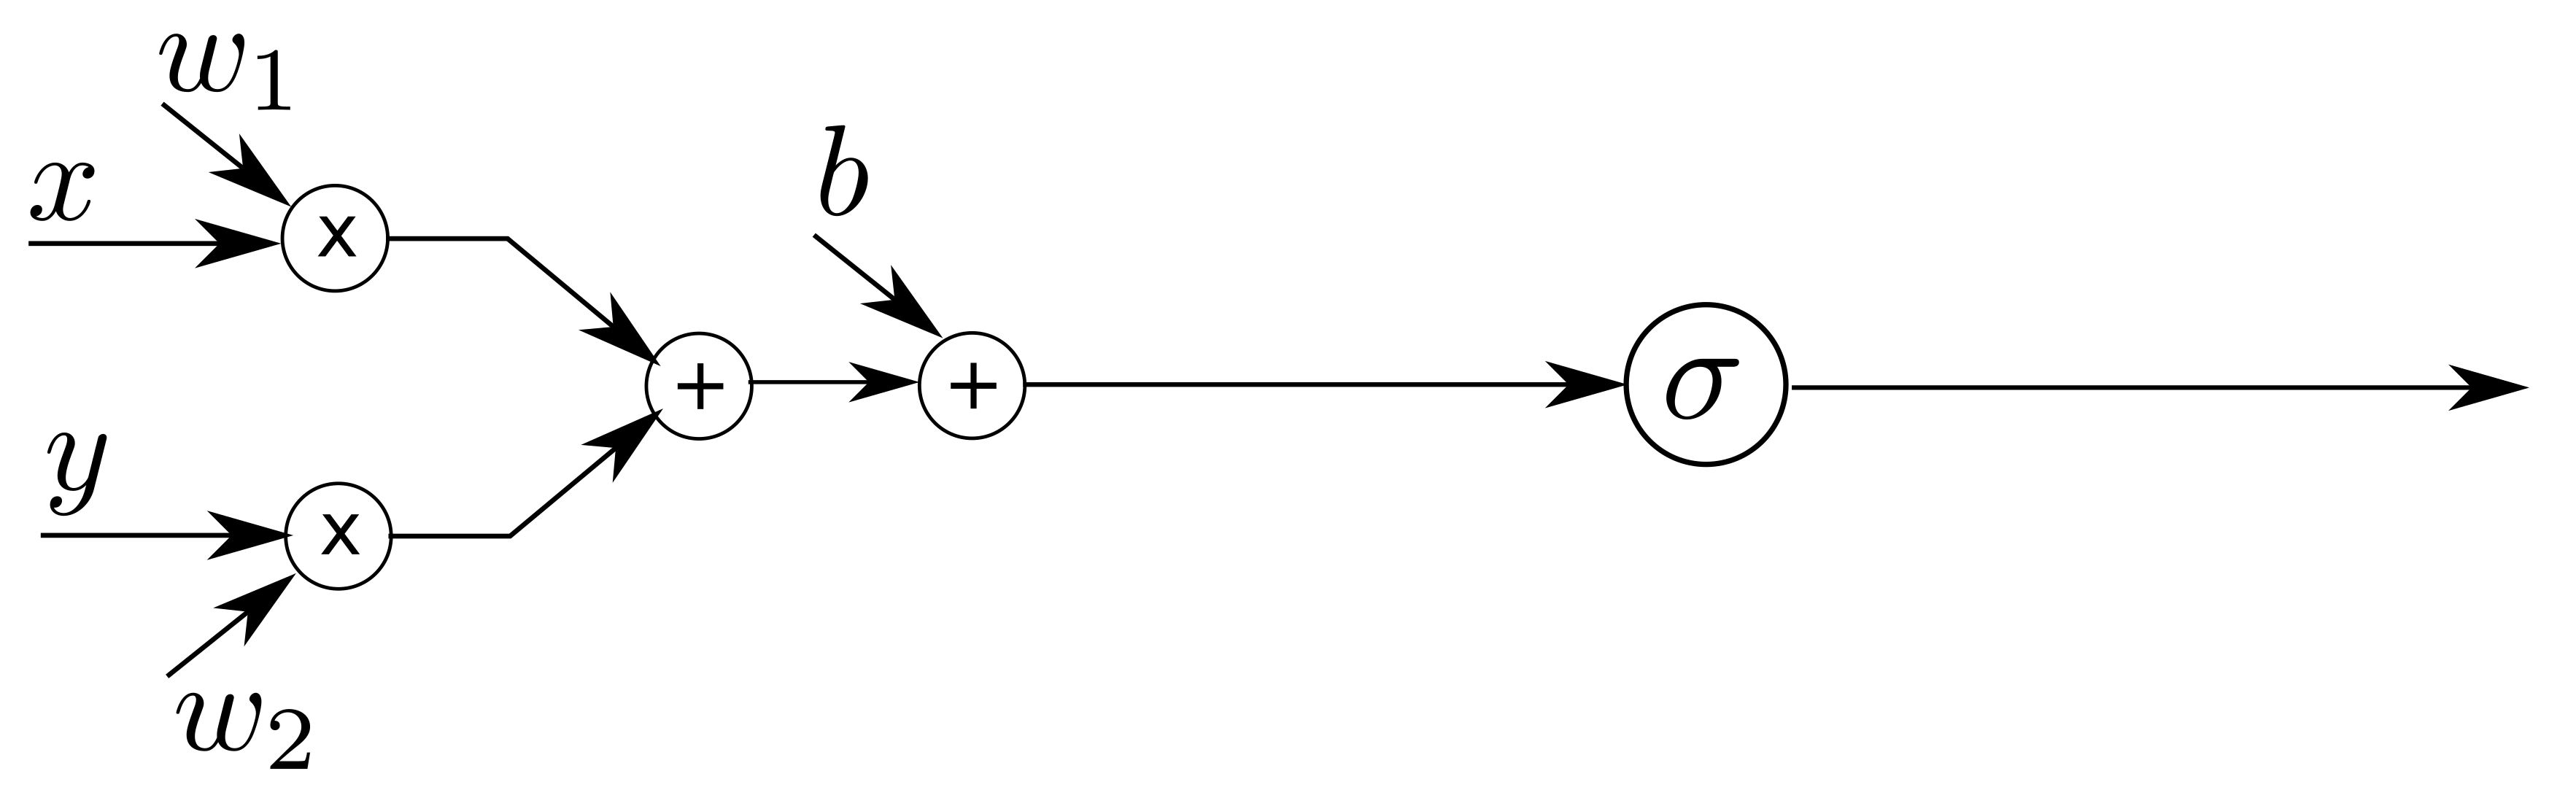
\includegraphics[width=0.7\textwidth]{comp_graph}

\end{frame}

%%%%%%%%%%%%%%%%%%%%%%%%%%%%%%%%%%%%
\begin{frame}{Setting the parameters of the computational graph}

  \begin{itemize}
  \item A \alert{computational graph} is used to compute a transformation between its inputs and outputs.
  \item In order to set its parameters, a loss function is chosen. Its minimization via gradient descent allows to set the parameters of the model.


    %% \alert{loss} function $\loss$, which depends on the input of the system $\X$ and its parameters $\param = \{\param_1, \ldots, \param_q\}$.

\end{itemize}

\end{frame}


%%%%%%%%%%%%%%%%%%%%%%%%%%%%%%%%%%%%
\begin{frame}{Gradient descent illustration (1D)}

\begin{columns}
  \begin{column}{.5\textwidth}
    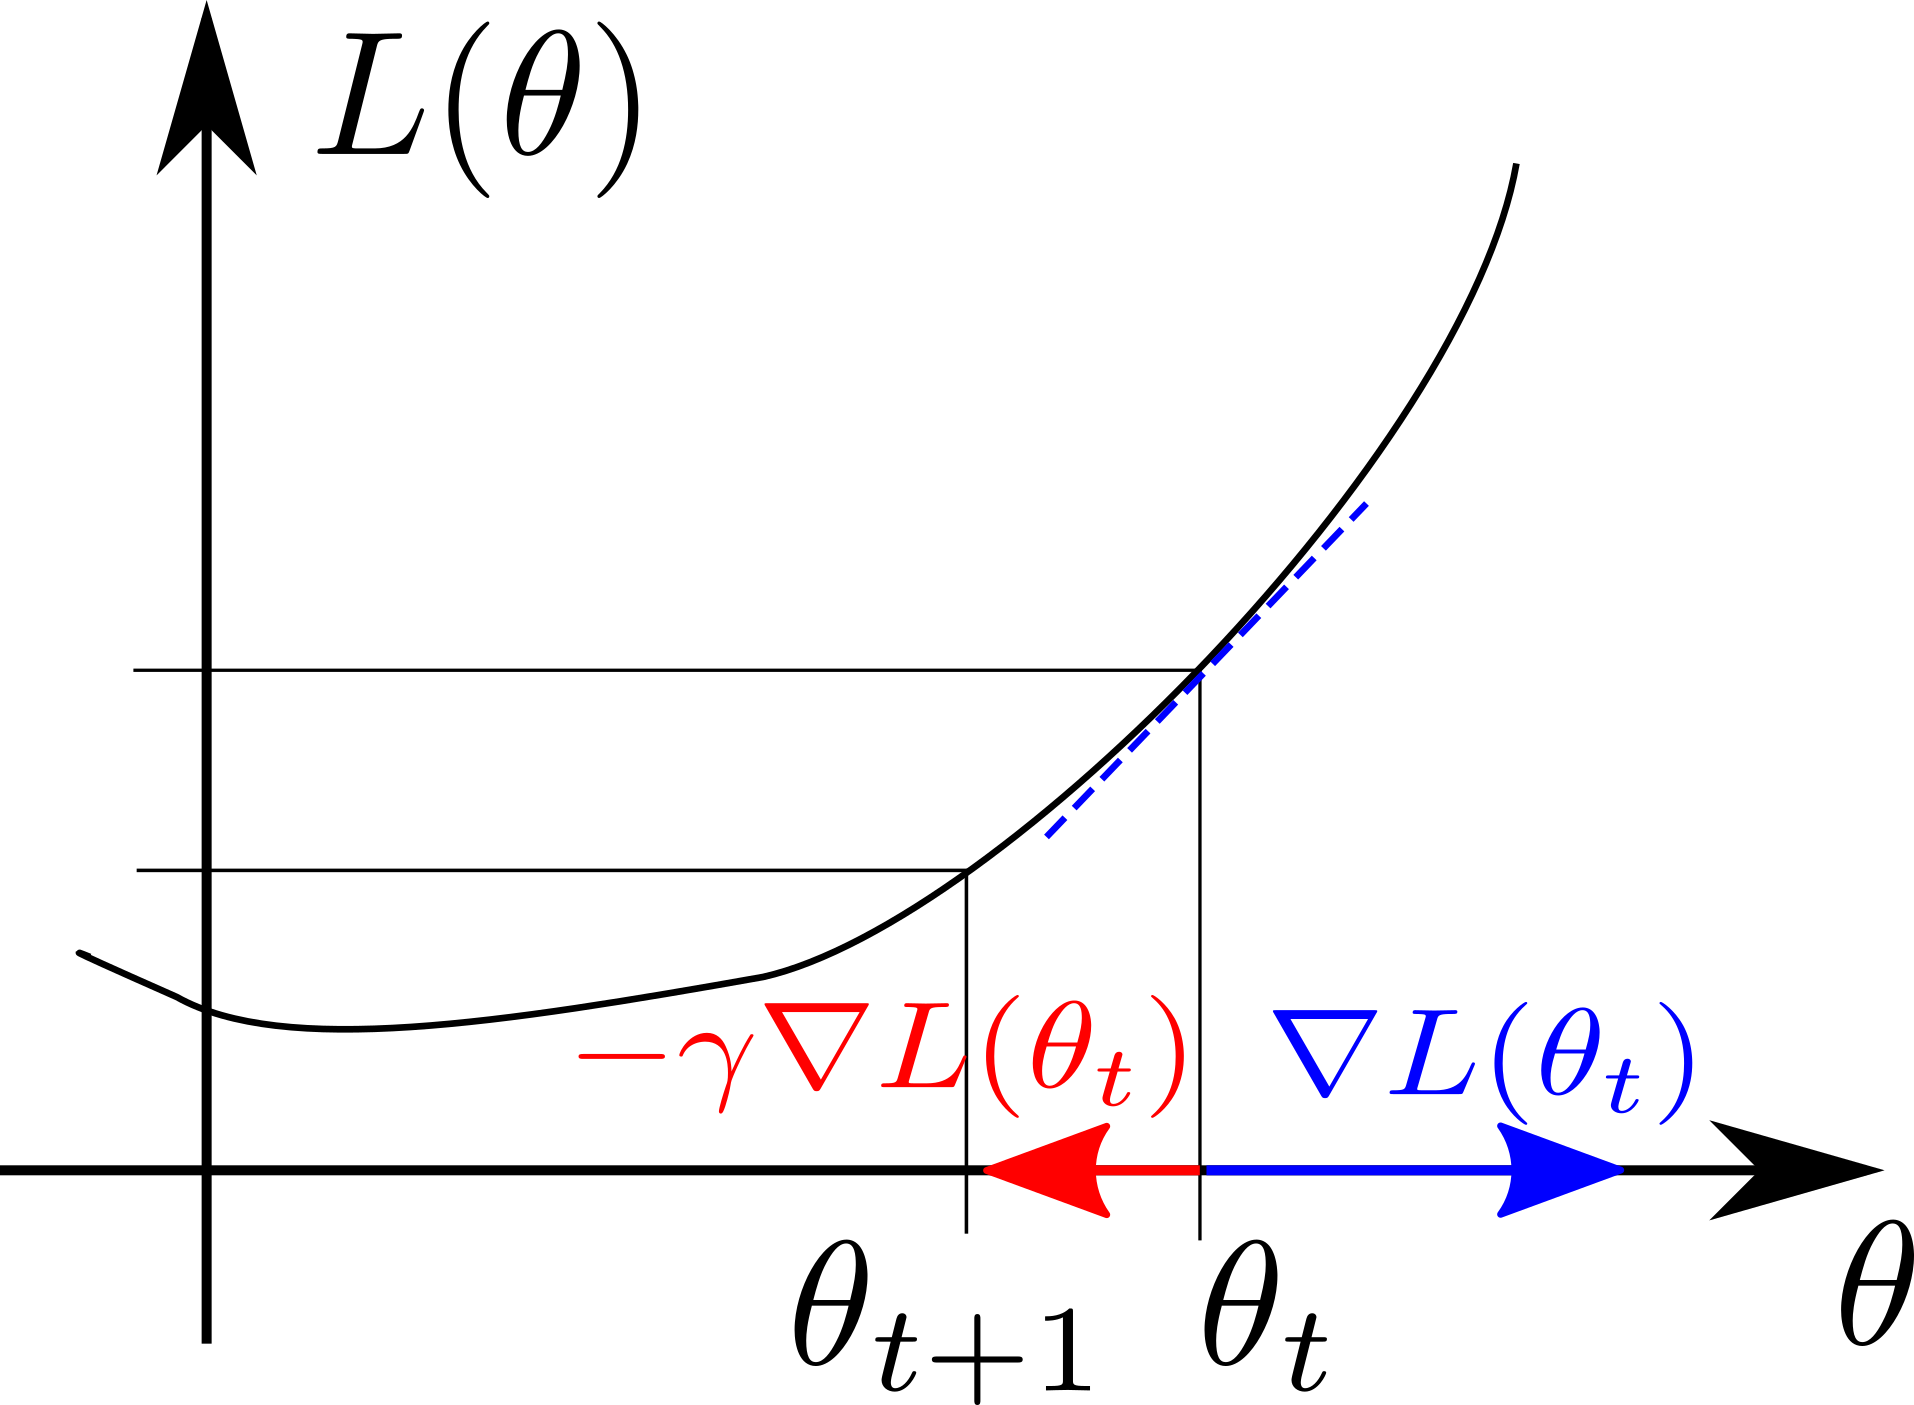
\includegraphics[width=\textwidth]{gradient_descent}
  \end{column}

  \begin{column}{.5\textwidth}
    \[
    \param_{t+1} = \param_t - \lr\nabla \loss(\param_t)
    \]
  \end{column}
\end{columns}

\end{frame}



%%%%%%%%%%%%%%%%%%%%%%%%%%%%%%%%%%%%
\begin{frame}{Gradient descent illustration (2D)}

  \begin{columns}
    \begin{column}{.6\textwidth}
      \begin{figure}
        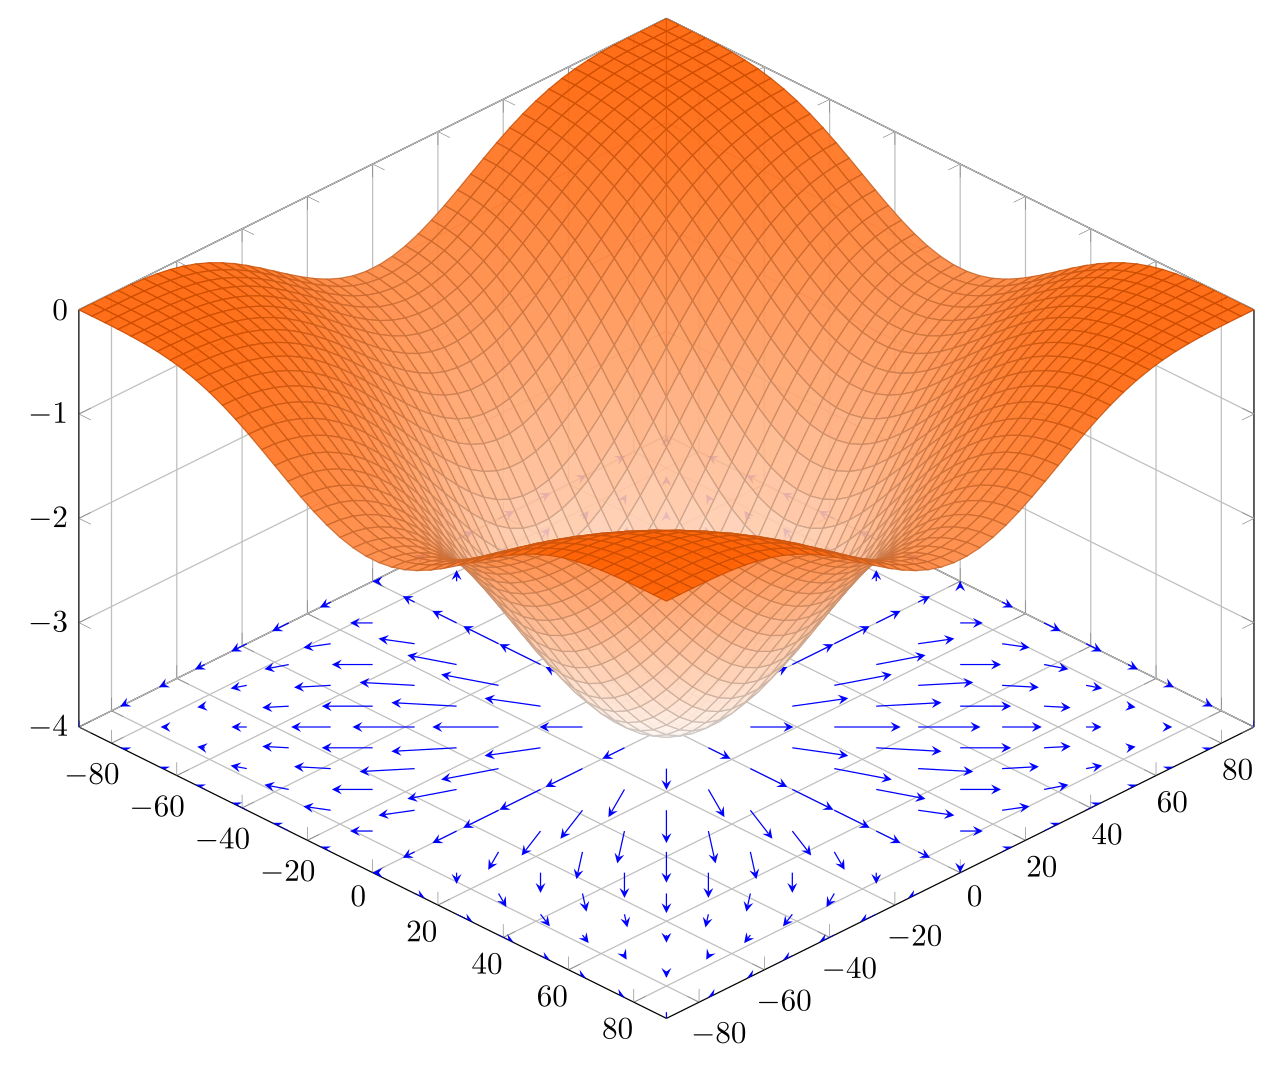
\includegraphics[height=5cm]{3d-gradient-cos.png}
        \source{By MartinThoma, CC0, https://commons.wikimedia.org/}
      \end{figure}
    \end{column}


    \begin{column}{.4\textwidth}
      \begin{block}{Definition: gradient}
        Let $\loss $ be a derivable function from $\R^n$ into $\R$. Its gradient $\nabla\loss$ is:
        \[
        \nabla_{\param} \loss (\param) =
        \begin{pmatrix}
          \frac{\partial \loss}{\partial \param_1}(\param)\\
          \vdots \\
          \frac{\partial \loss}{\partial \param_n}(\param)
        \end{pmatrix}
        \]

      \end{block}
    \end{column}
  \end{columns}


\end{frame}


%%%%%%%%%%%%%%%%%%%%%%%%%%%%%%%%%%%%
\begin{frame}{Gradient descent applied to computational graphs}

  In the case of computational graphs, the loss $\loss$ depends on each parameter $\param_i$ via the composition of several functions. In order to compute the gradient $\nabla_{\param}\loss$ we will make extensive use of the chain rule theorem.

  \begin{block}{Chain rule theorem}
    Let $f_1$ and $f_2$ be two differentiable real functions ($\R \rightarrow \R$). Then for all $x$ in $\R$:   :
    \[
     (f_2 \circ f_1)'(x) = f_2'(f_1(x)).f_1'(x)
    \]
  \end{block}


\begin{block}{Leibniz notation}
  Let us introduce variables $x$, $y$ and $z$:
  \[x \xrightarrow{f_1} y \xrightarrow{f_2} z\]

  Then:
  \[\dv{z}{x} = \dv{z}{y} \cdot \dv{y}{x} \]

\end{block}

\end{frame}


%%%%%%%%%%%%%%%%%%%%%%%%%%%%%%%%%%%%
\begin{frame}{The backpropagation algorithm}

  \begin{itemize}
  \item The backpropagation algorithm is used in a computational graph to efficiently compute the partial derivatives of the loss with respect to each parameter of the network.
  \item One can trace the origins of the method to the sixties
  \item It was first applied to NN in the eighties \cite{werbos_applications_1982, lecun_procedure_1985}
  \end{itemize}


\end{frame}


%%%%%%%%%%%%%%%%%%%%%%%%%%%%%%%%%%%%
\begin{frame}{The backpropagation algorithm: intuition}

  \begin{itemize}
  \item Given a computational graph, the main idea is to compute the local partial derivatives during a forward pass
    \item Then, during a backward pass, the partial derivatives of the loss with respect to each parameter is computed
  \end{itemize}


\end{frame}





%%%%%%%%%%%%%%%%%%%%%%%%%%%%%%%%%%%%
\begin{frame}<handout>{Simple backpropagation example}

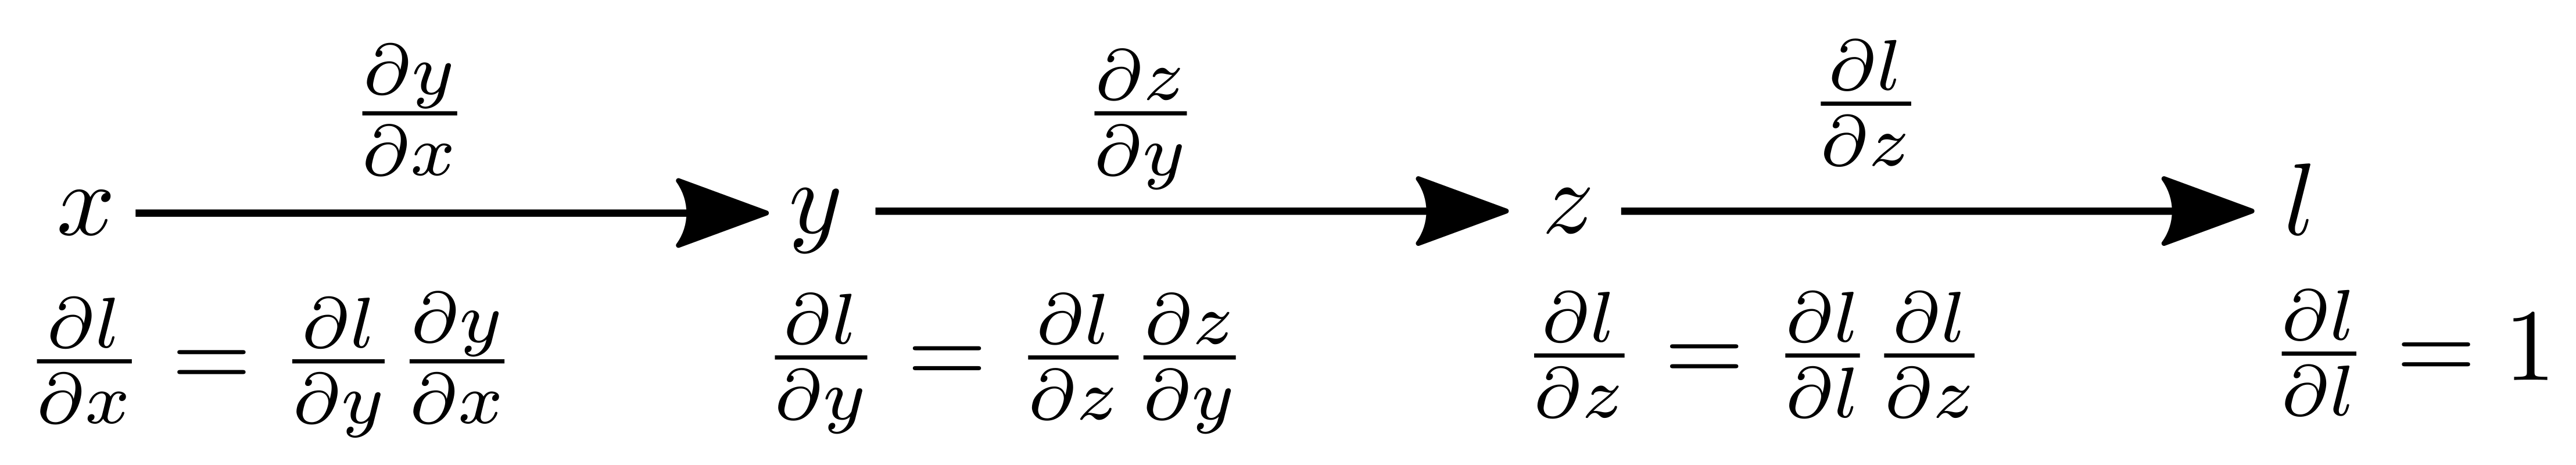
\includegraphics[width=\textwidth]{bp_simple.png}

\end{frame}

%%%%%%%%%%%%%%%%%%%%%%%%%%%%%%%%%%%%
\begin{frame}<beamer>{Simple backpropagation example}

\only<1>{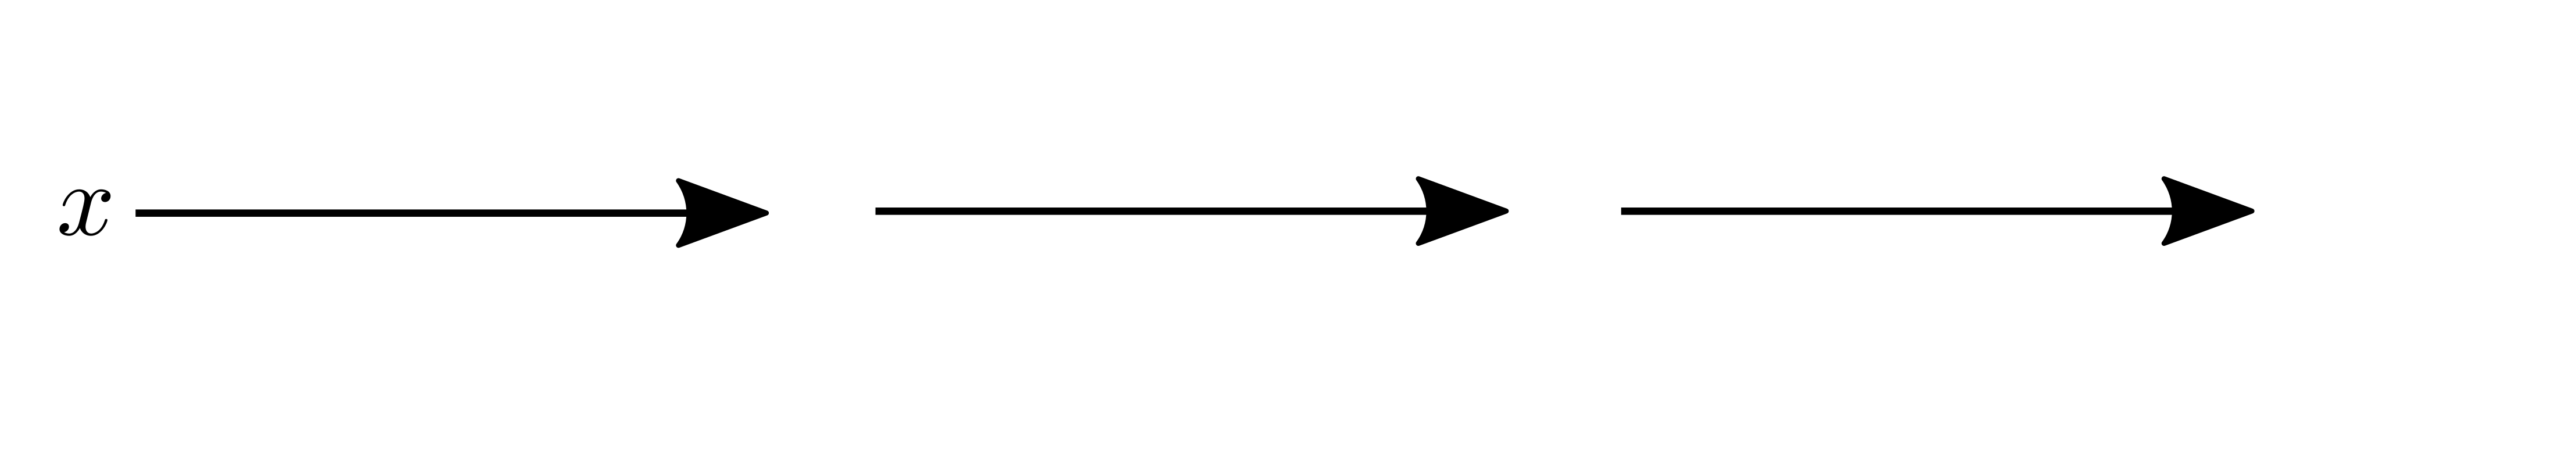
\includegraphics[width=\textwidth]{bp_simple_1.png}}
\only<2>{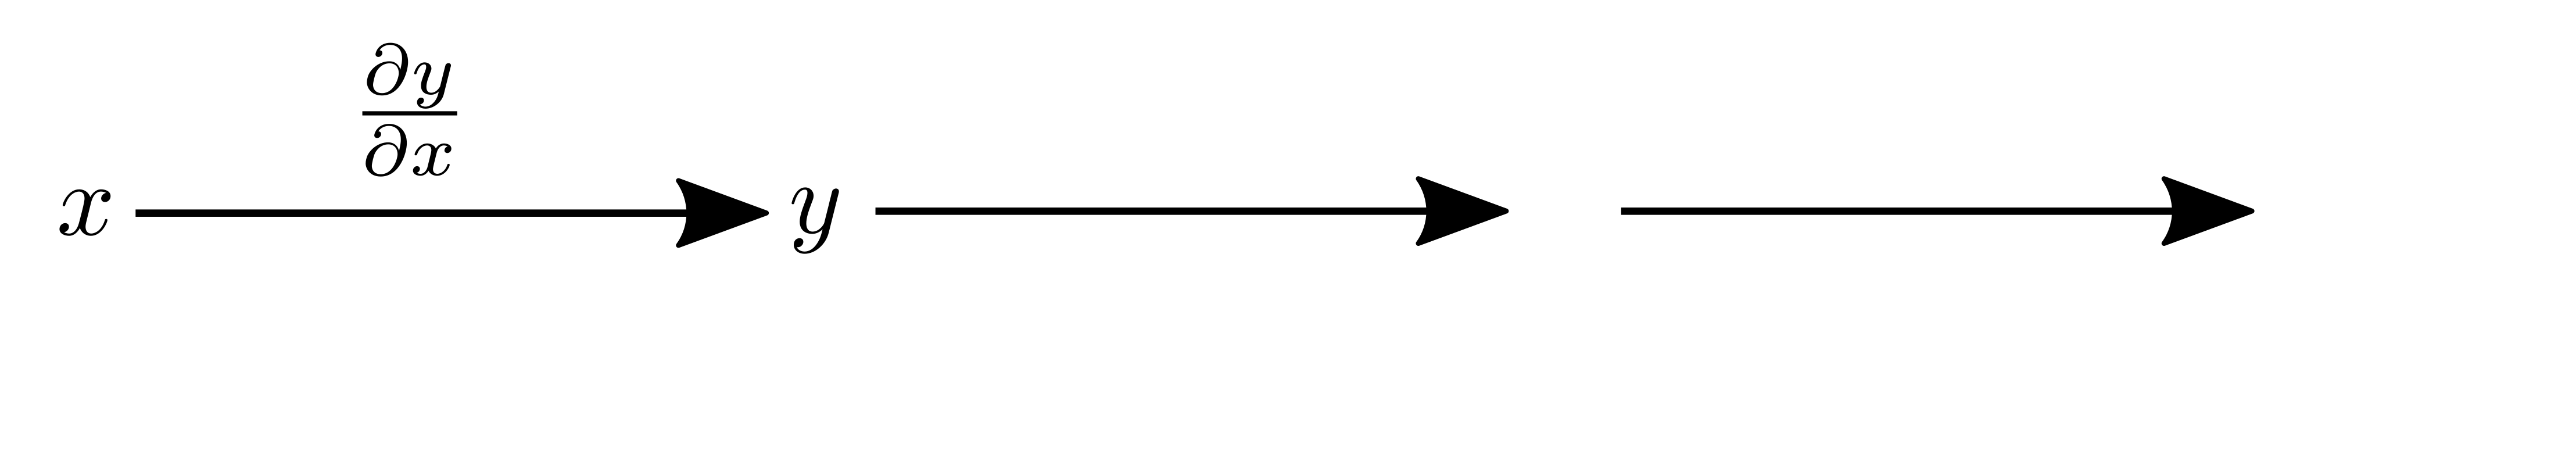
\includegraphics[width=\textwidth]{bp_simple_2.png}}
\only<3>{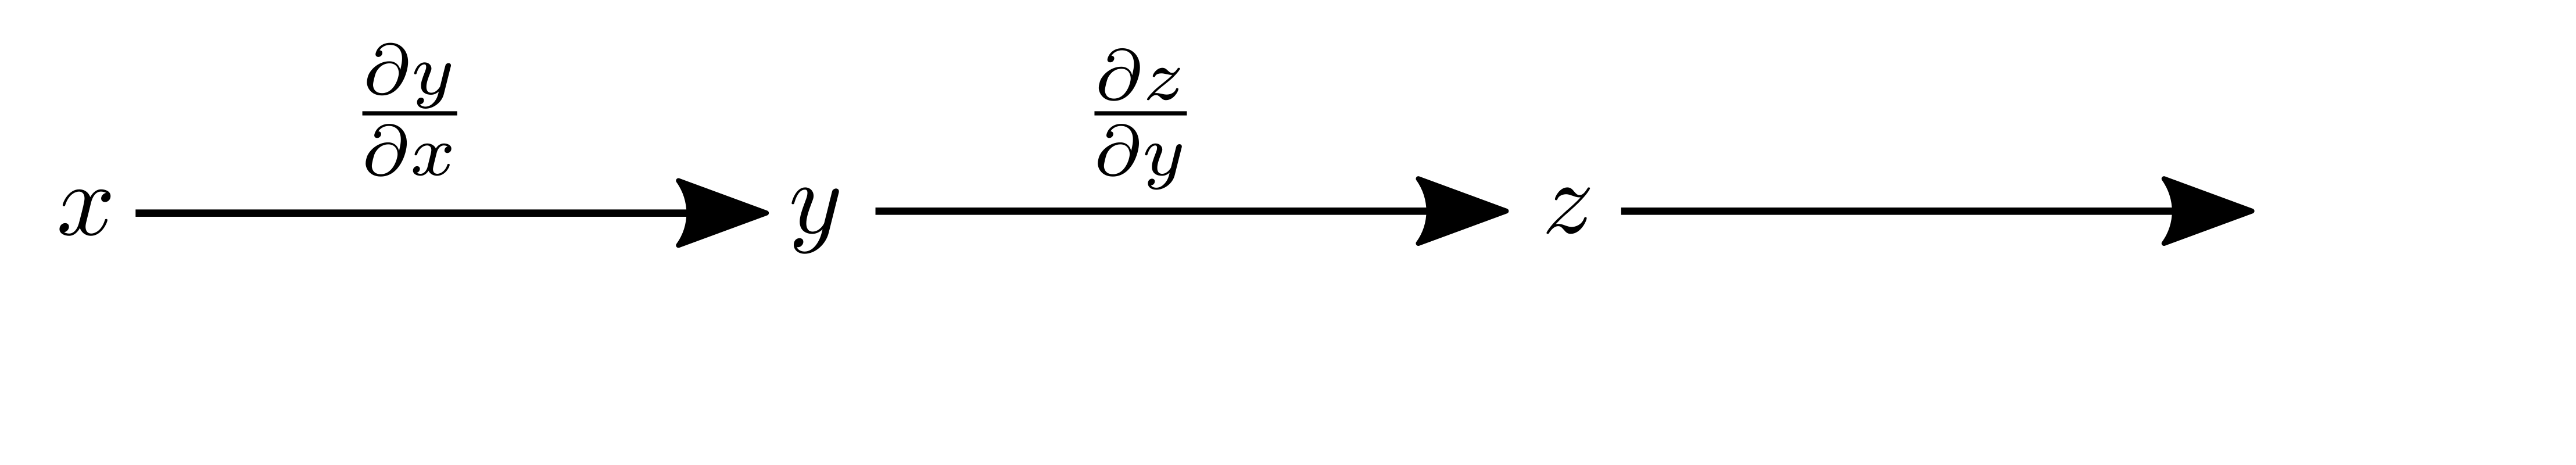
\includegraphics[width=\textwidth]{bp_simple_3.png}}
\only<4>{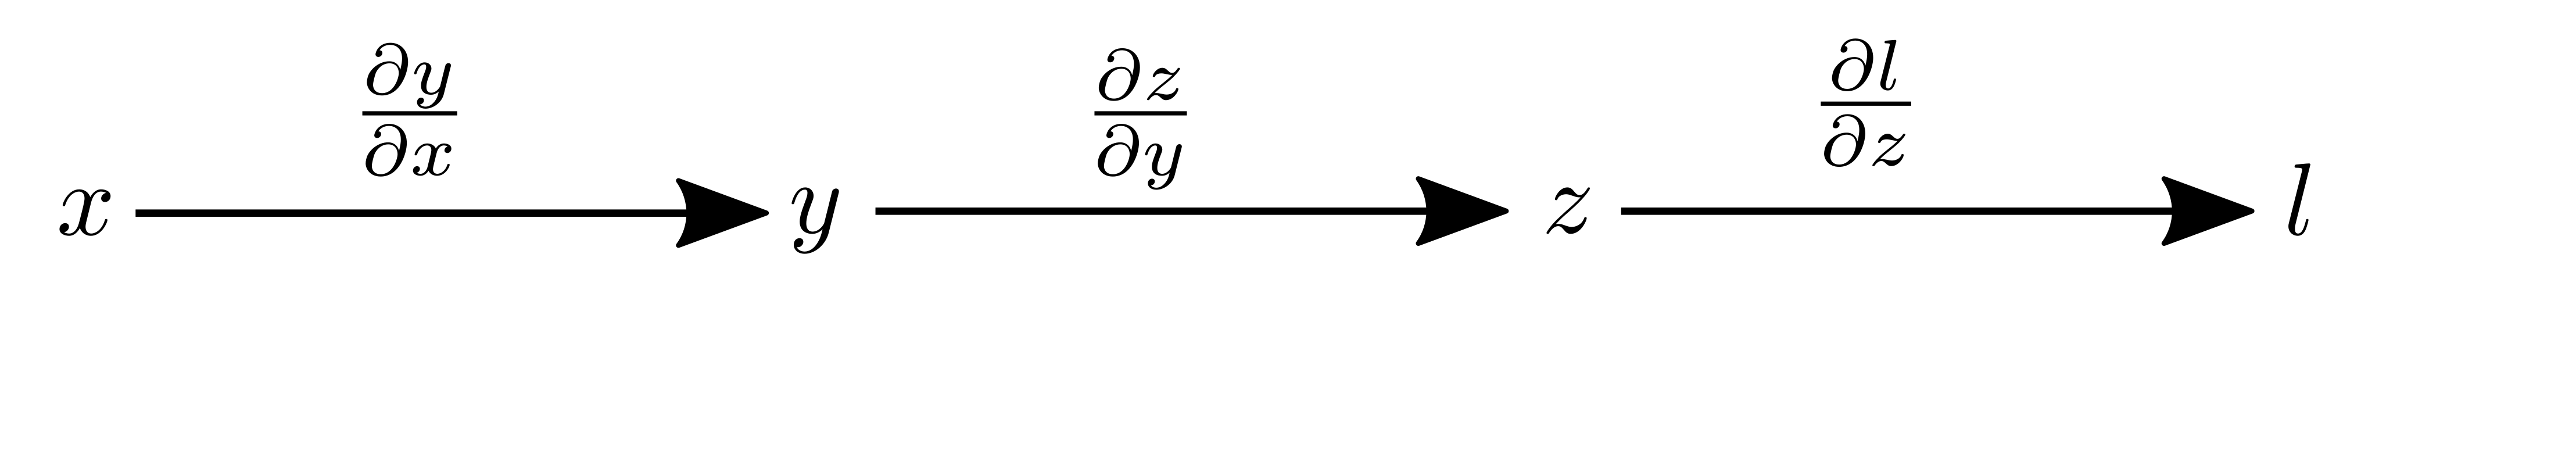
\includegraphics[width=\textwidth]{bp_simple_4.png}}
\only<5>{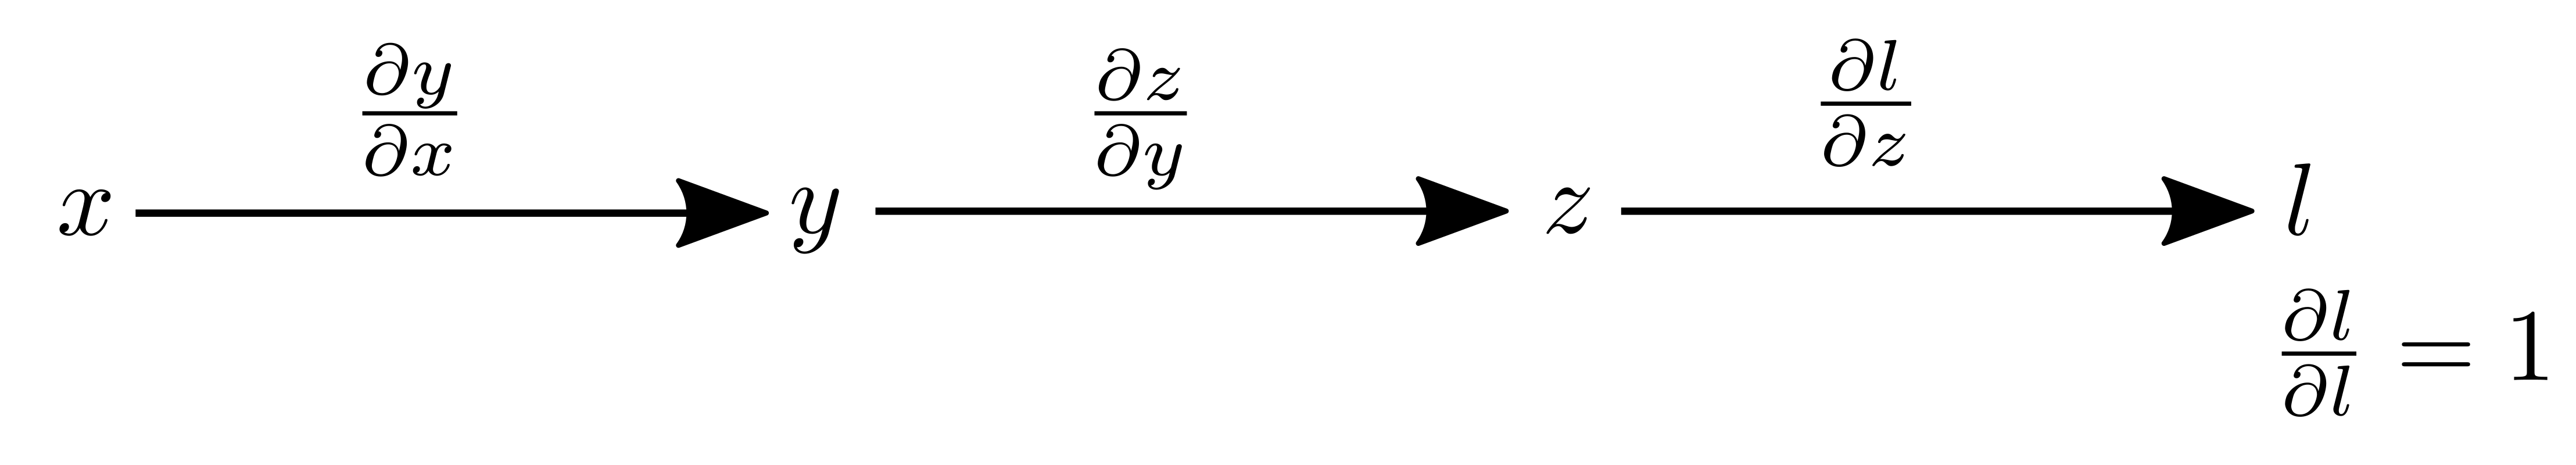
\includegraphics[width=\textwidth]{bp_simple_5.png}}
\only<6>{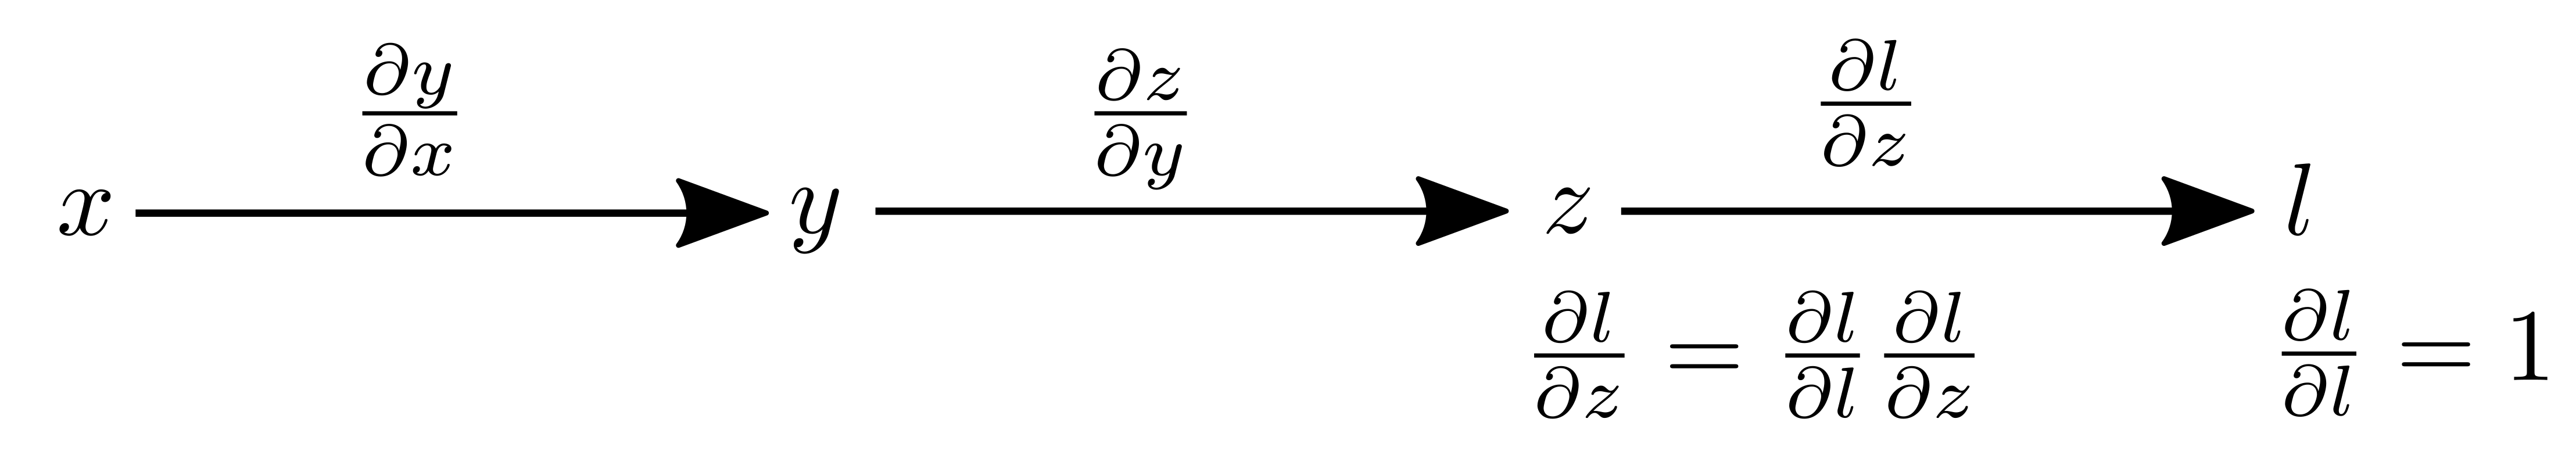
\includegraphics[width=\textwidth]{bp_simple_6.png}}
\only<7>{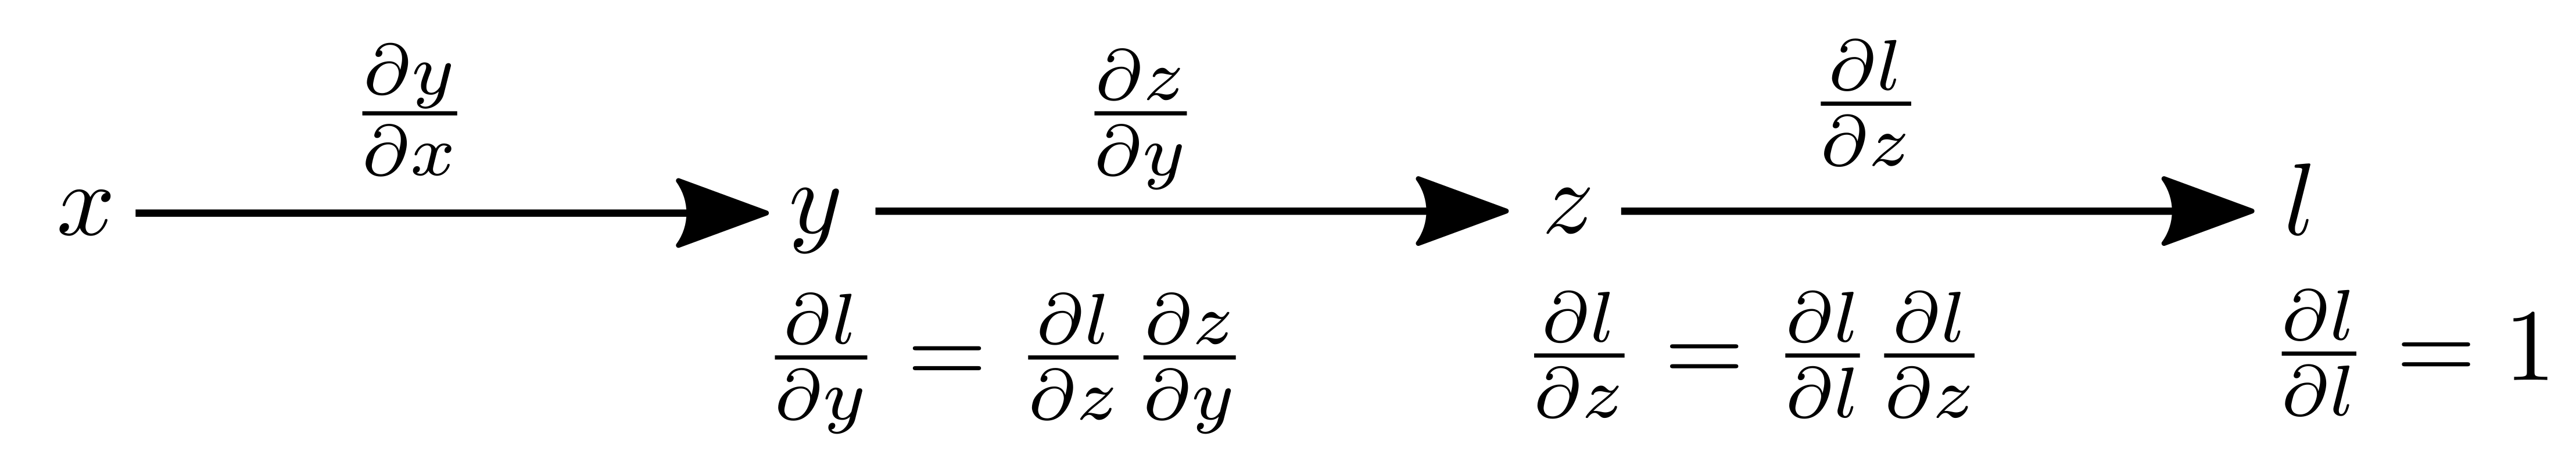
\includegraphics[width=\textwidth]{bp_simple_7.png}}
\only<8>{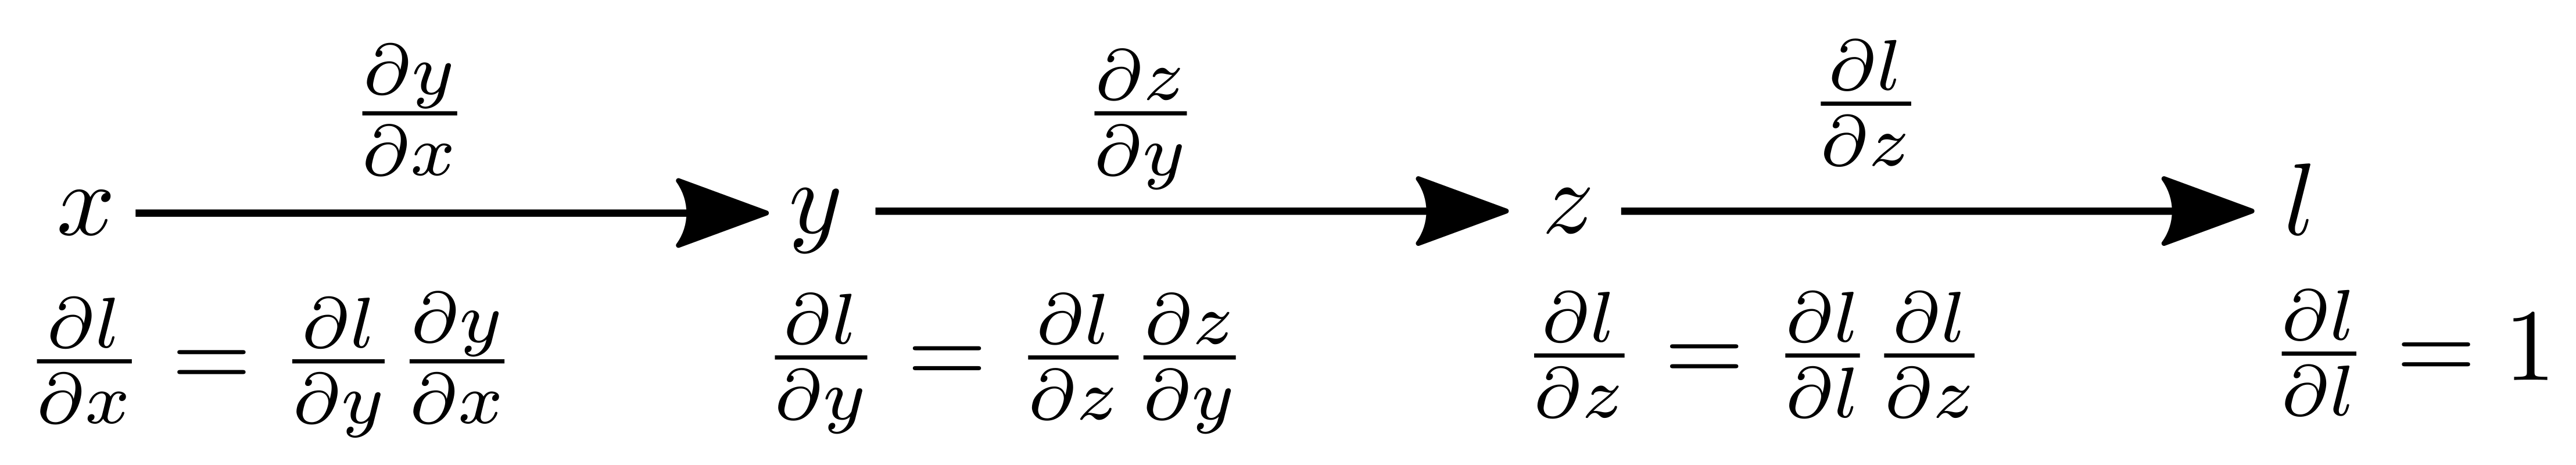
\includegraphics[width=\textwidth]{bp_simple_8.png}}

\end{frame}

%%%%%%%%%%%%%%%%%%%%%%%%%%%%%%%%%%%%%%%%%%%%%%%%%%
\frame{
\frametitle{Feed-forward neural networks}

\begin{block}{Definition}
  \begin{itemize}
  \item A feed-forward neural networks is a computational graph
  \item Its computing units, the neurons, are organized in \alert{layers}
  \end{itemize}

\end{block}

\begin{figure}
  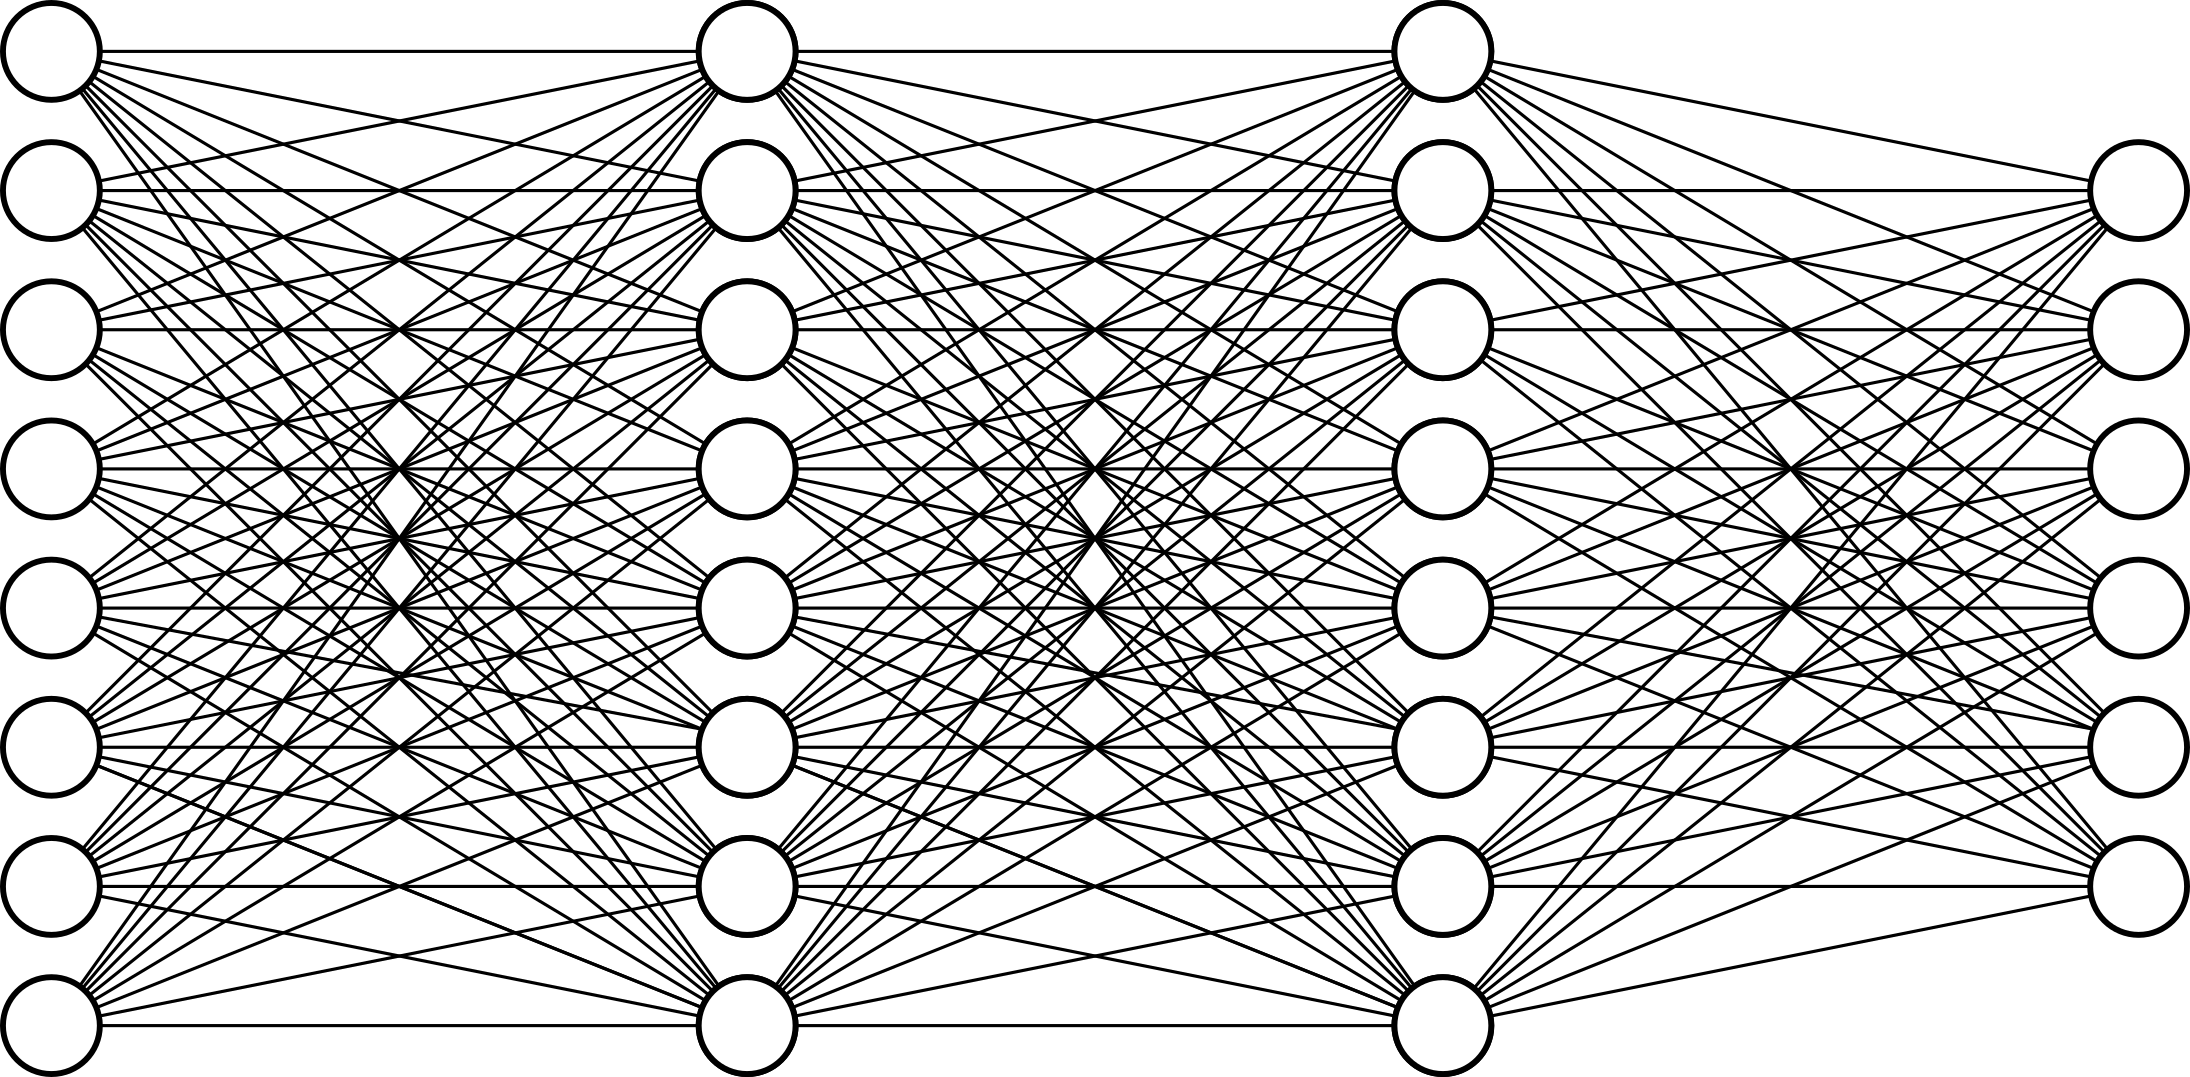
\includegraphics[height=3cm]{mini_reseau3_bis.png}
\end{figure}


}


%%%%%%%%%%%%%%%%%%%%%%%%%%%%%%%%%%%%
\begin{frame}{Artificial neuron}

    \begin{figure}
      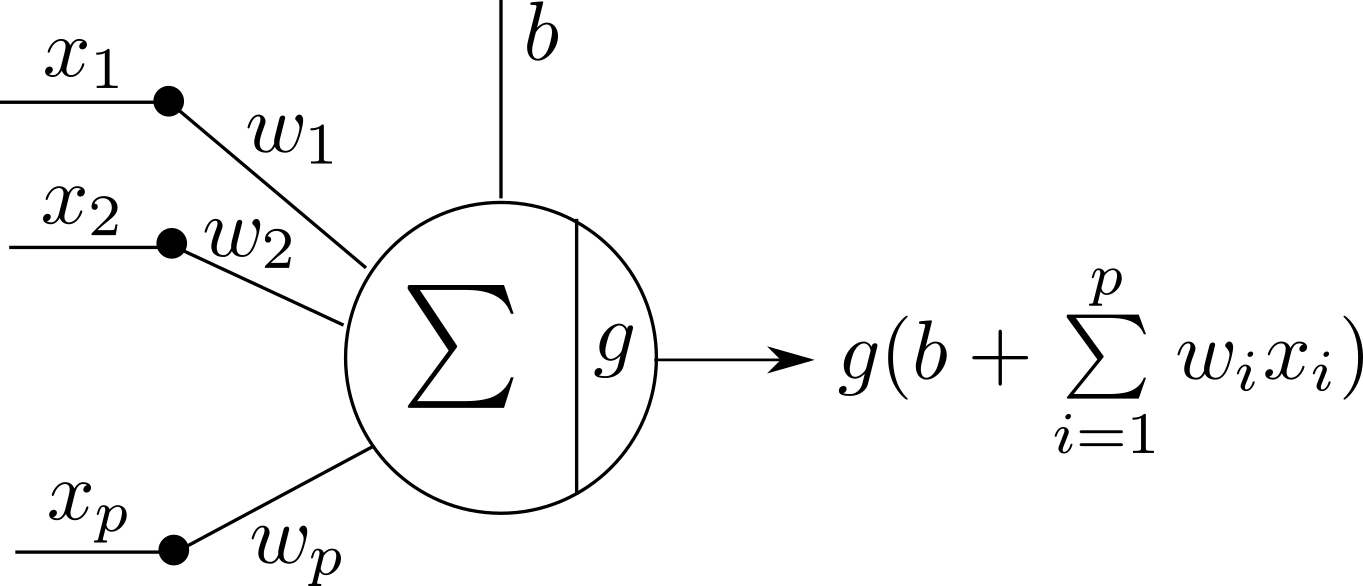
\includegraphics[height=3cm]{neurone_representation_compacte}
    \end{figure}

\end{frame}

%%%%%%%%%%%%%%%%%%%%%%%%%%%%%%%%%%%%%%%%%%%%%%
\frame{
\frametitle{Notations}

\begin{columns}

  \begin{column}{.5\textwidth}
\begin{figure}
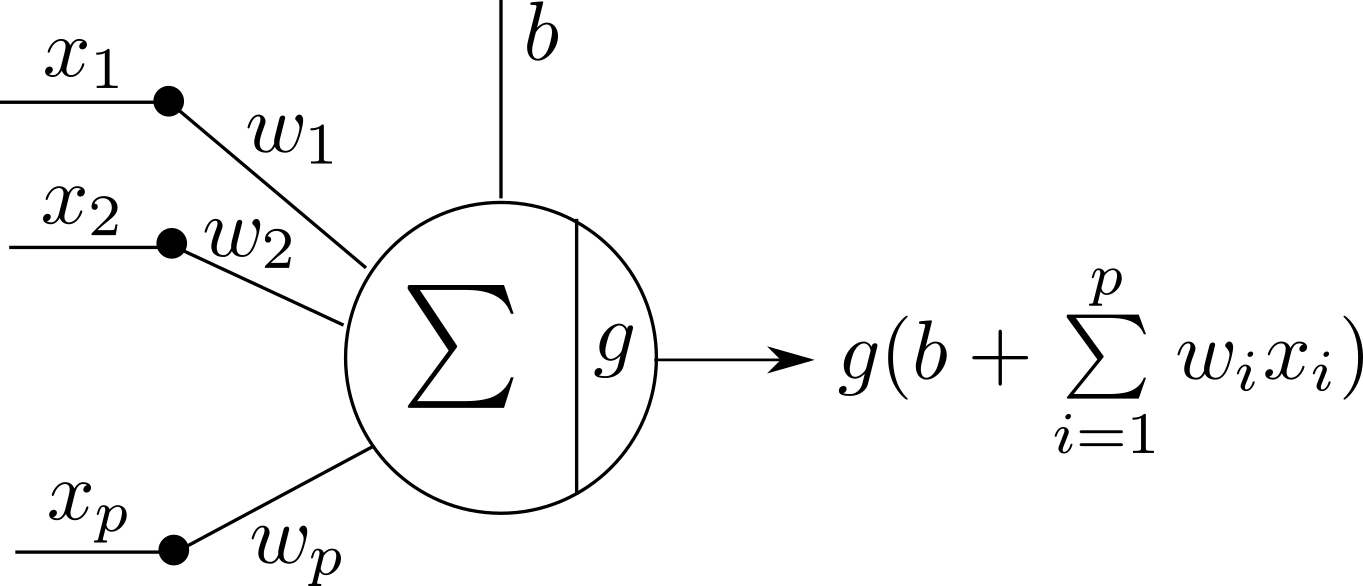
\includegraphics[height=2cm]{neurone_representation_compacte}
\end{figure}
\end{column}

  \begin{column}{.5\textwidth}
  With
  \[
  \mathbf{w} =
  \begin{pmatrix}
    w_1 \\
    \vdots \\
    w_p
  \end{pmatrix}
  = (w_1, \ldots, w_p)^T
  \]
  and
  \[
  \x =
  \begin{pmatrix}
    x_1 \\
    \vdots \\
    x_p
  \end{pmatrix}
  = (x_1, \ldots, x_p)^T
  \]
\end{column}

\end{columns}

We can simply write:
\[
\act(b+ \sum\limits_{i=1}^p w_ix_i) = \act(b + \mathbf{w}^T\x)
\]

}

%%%%%%%%%%%%%%%%%%%%%%%%%%%%%%%%%%%%%%%%%%%%%%%%%%

\frame{
  \frametitle{Activation: sigmoid}

  \begin{columns}
    \begin{column}{.5\textwidth}
      \[
      \act(x)= \frac{1}{1 + e^{-x}}
      \]
    \end{column}

    \begin{column}{.5\textwidth}
      \begin{figure}
        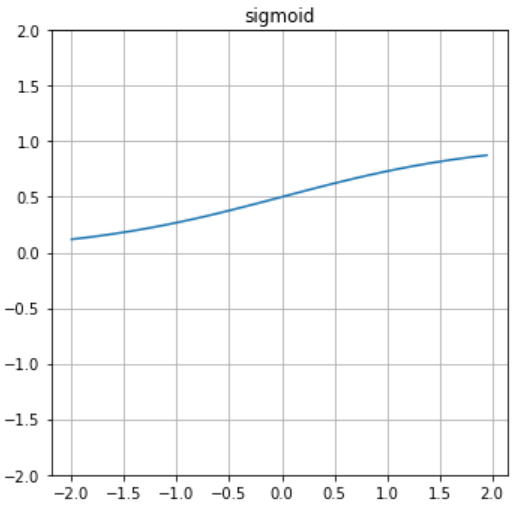
\includegraphics[width=.8\textwidth]{act_sigm.png}
      \end{figure}


    \end{column}
  \end{columns}

  \begin{block}{Remarks}
    \begin{itemize}
    \item[+] Similar to binary activation, but with usable gradient
    \item[-] However, gradient tends to zero when input is far from zero
    \item[-] More computationally intensive
    \end{itemize}
  \end{block}



}

%%%%%%%%%%%%%%%%%%%%%%%%%%%%%%%%%%%%%%%%%%%%%%%%%%

%% \frame{
%%   \frametitle{Activation: hyperbolic tangent}

%%   \begin{columns}
%%     \begin{column}{.5\textwidth}
%%       \[
%%       \act(x)= \frac{e^x - e^{-x}}{e^x + e^{-x}}
%%       \]
%%     \end{column}

%%     \begin{column}{.5\textwidth}
%%       \begin{figure}
%%         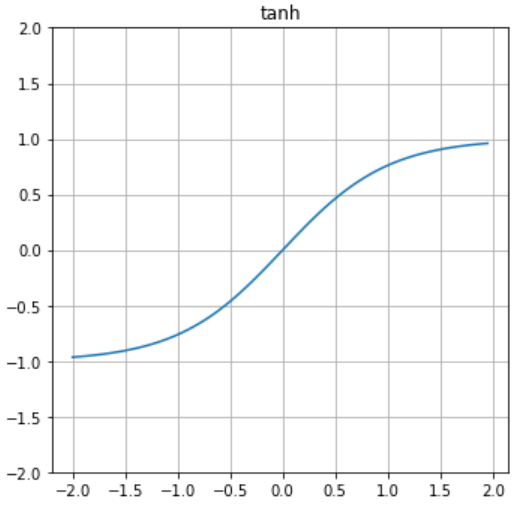
\includegraphics[width=.8\textwidth]{act_tanh.png}
%%       \end{figure}


%%     \end{column}
%%   \end{columns}

%%   \begin{block}{Remarks}
%%     \begin{itemize}
%%     \item Similar to sigmoid
%%     \end{itemize}
%%   \end{block}



%% }


%%%%%%%%%%%%%%%%%%%%%%%%%%%%%%%%%%%%%%%%%%%%%%%%%%

\frame{
  \frametitle{Activation: rectified linear unit (ReLU)}

  \begin{columns}
    \begin{column}{.5\textwidth}
      \[
      \act(x)=
      \begin{cases}
        x,& \text{if } x > 0\\
        0,              & \text{otherwise}
      \end{cases}
      \]
    \end{column}

    \begin{column}{.5\textwidth}
      \begin{figure}
        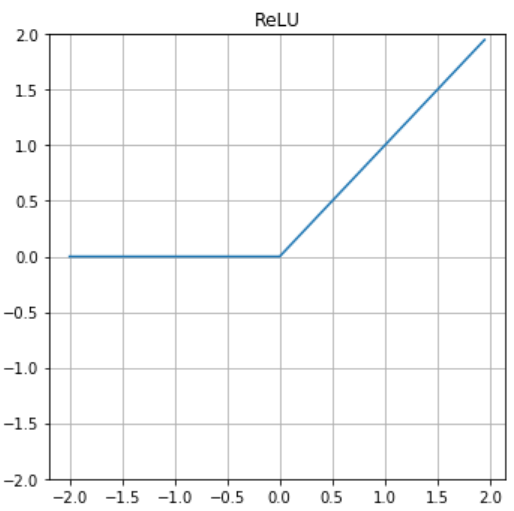
\includegraphics[width=.8\textwidth]{act_relu.png}
      \end{figure}


    \end{column}
  \end{columns}

  \begin{block}{Remarks}
    \begin{itemize}
    \item[+] Usable gradient when activated
    \item[+] Fast to compute
    \item[+] High abstraction
    \end{itemize}
  \end{block}

\pause

  \begin{alertblock}{}
    ReLU is the most commonly used activation function.
  \end{alertblock}


}


%%%%%%%%%%%%%%%%%%%%%%%%%%%%%%%%%%%%%%%%%%%%%%%%%%
\frame{
\frametitle{Fully-connected layer}

\begin{itemize}
\item A layer is said to be fully-connected (FC) if each of its neurons is connected to all the neurons of the previous layer
  \item  If a FC layer contains $r$ neurons, and the previous layer $q$, then its weights are a 2D dimensional array (a matrix) of size $q \times r$
\end{itemize}

\begin{figure}
  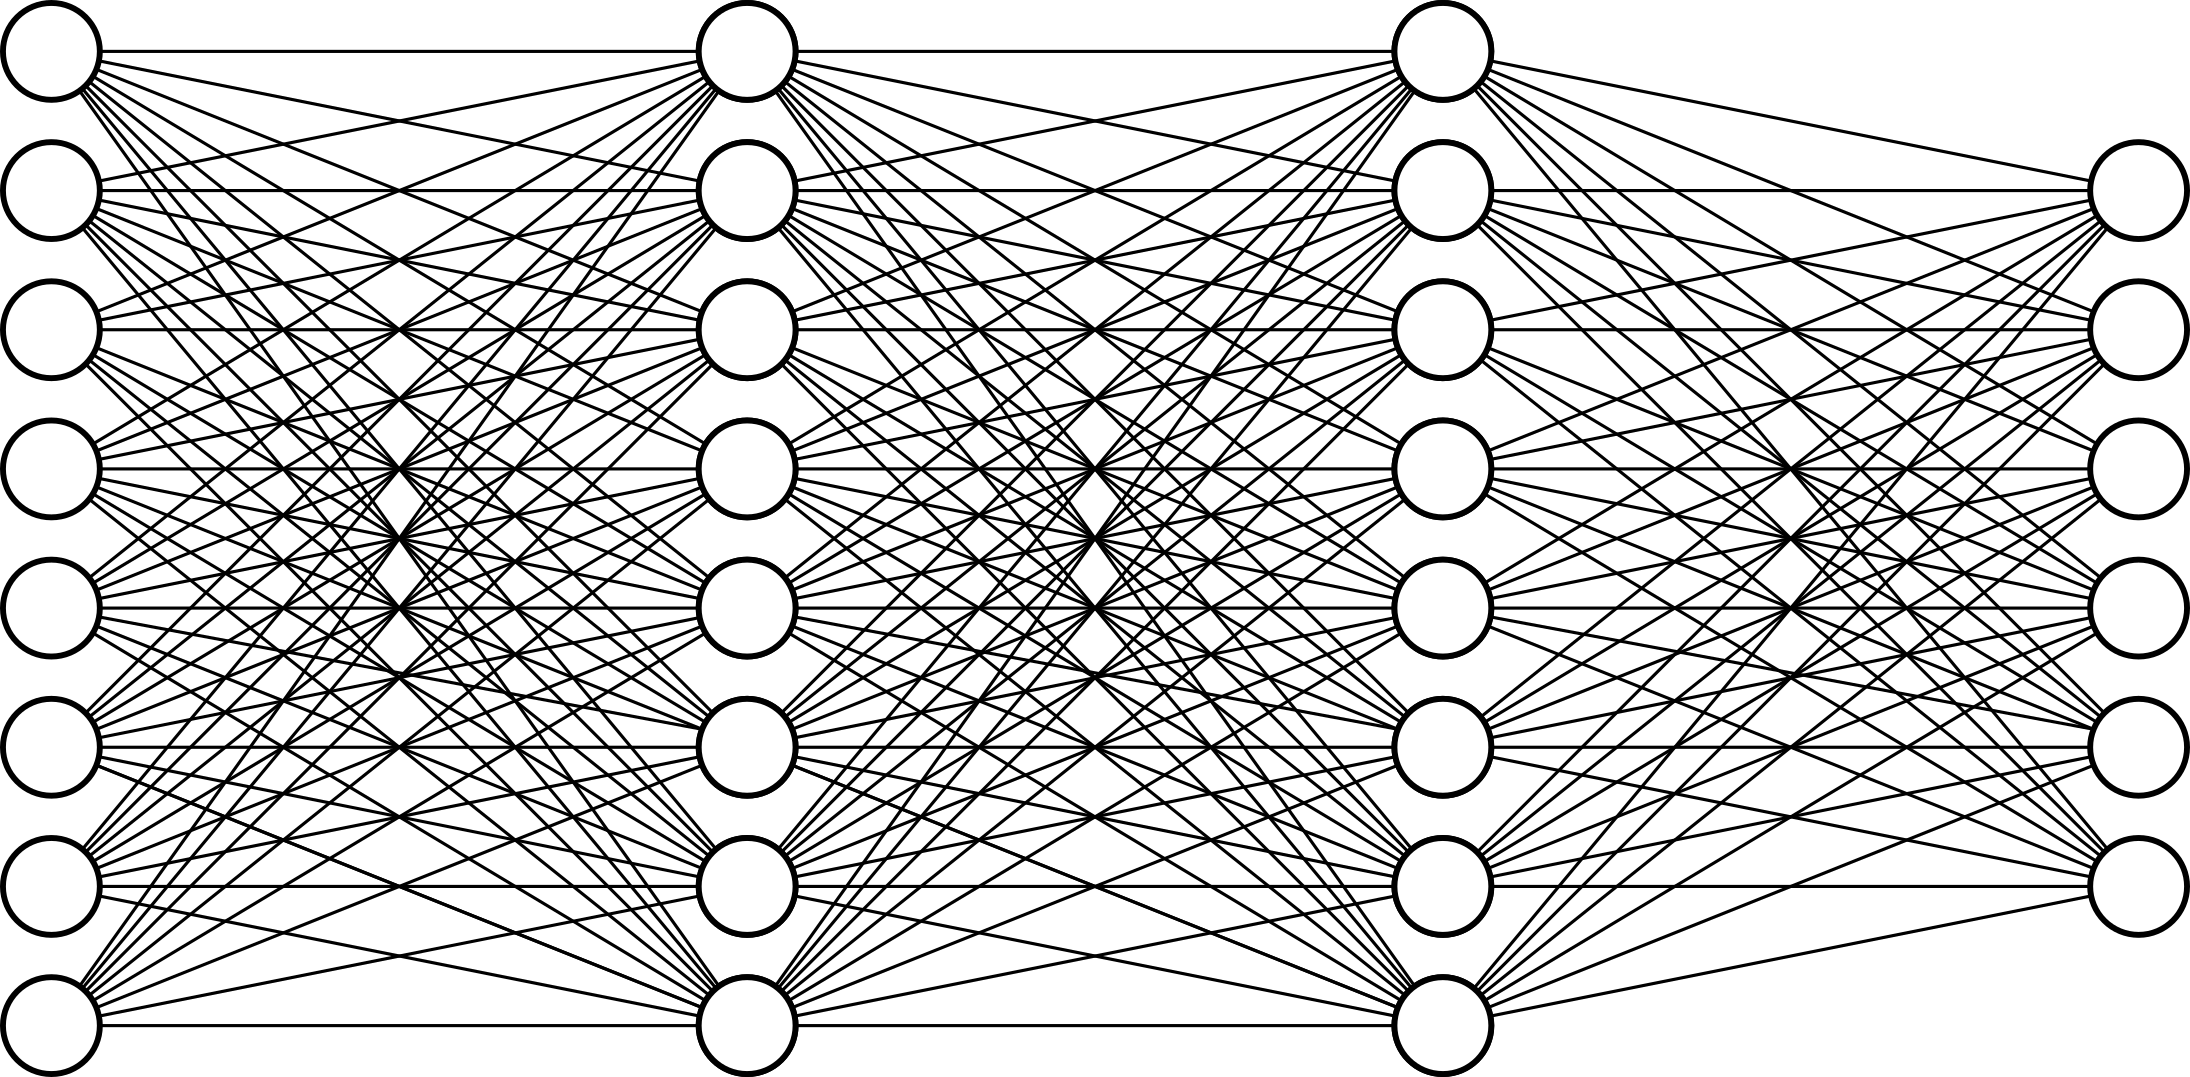
\includegraphics[height=3cm]{mini_reseau3_bis.png}
\end{figure}

}


%%%%%%%%%%%%%%%%%%%%%%%%%%%%%%%%%%%%
\begin{frame}{Graphical representation of NNs}

\begin{columns}
  \begin{column}{.5\textwidth}
    \begin{figure}
      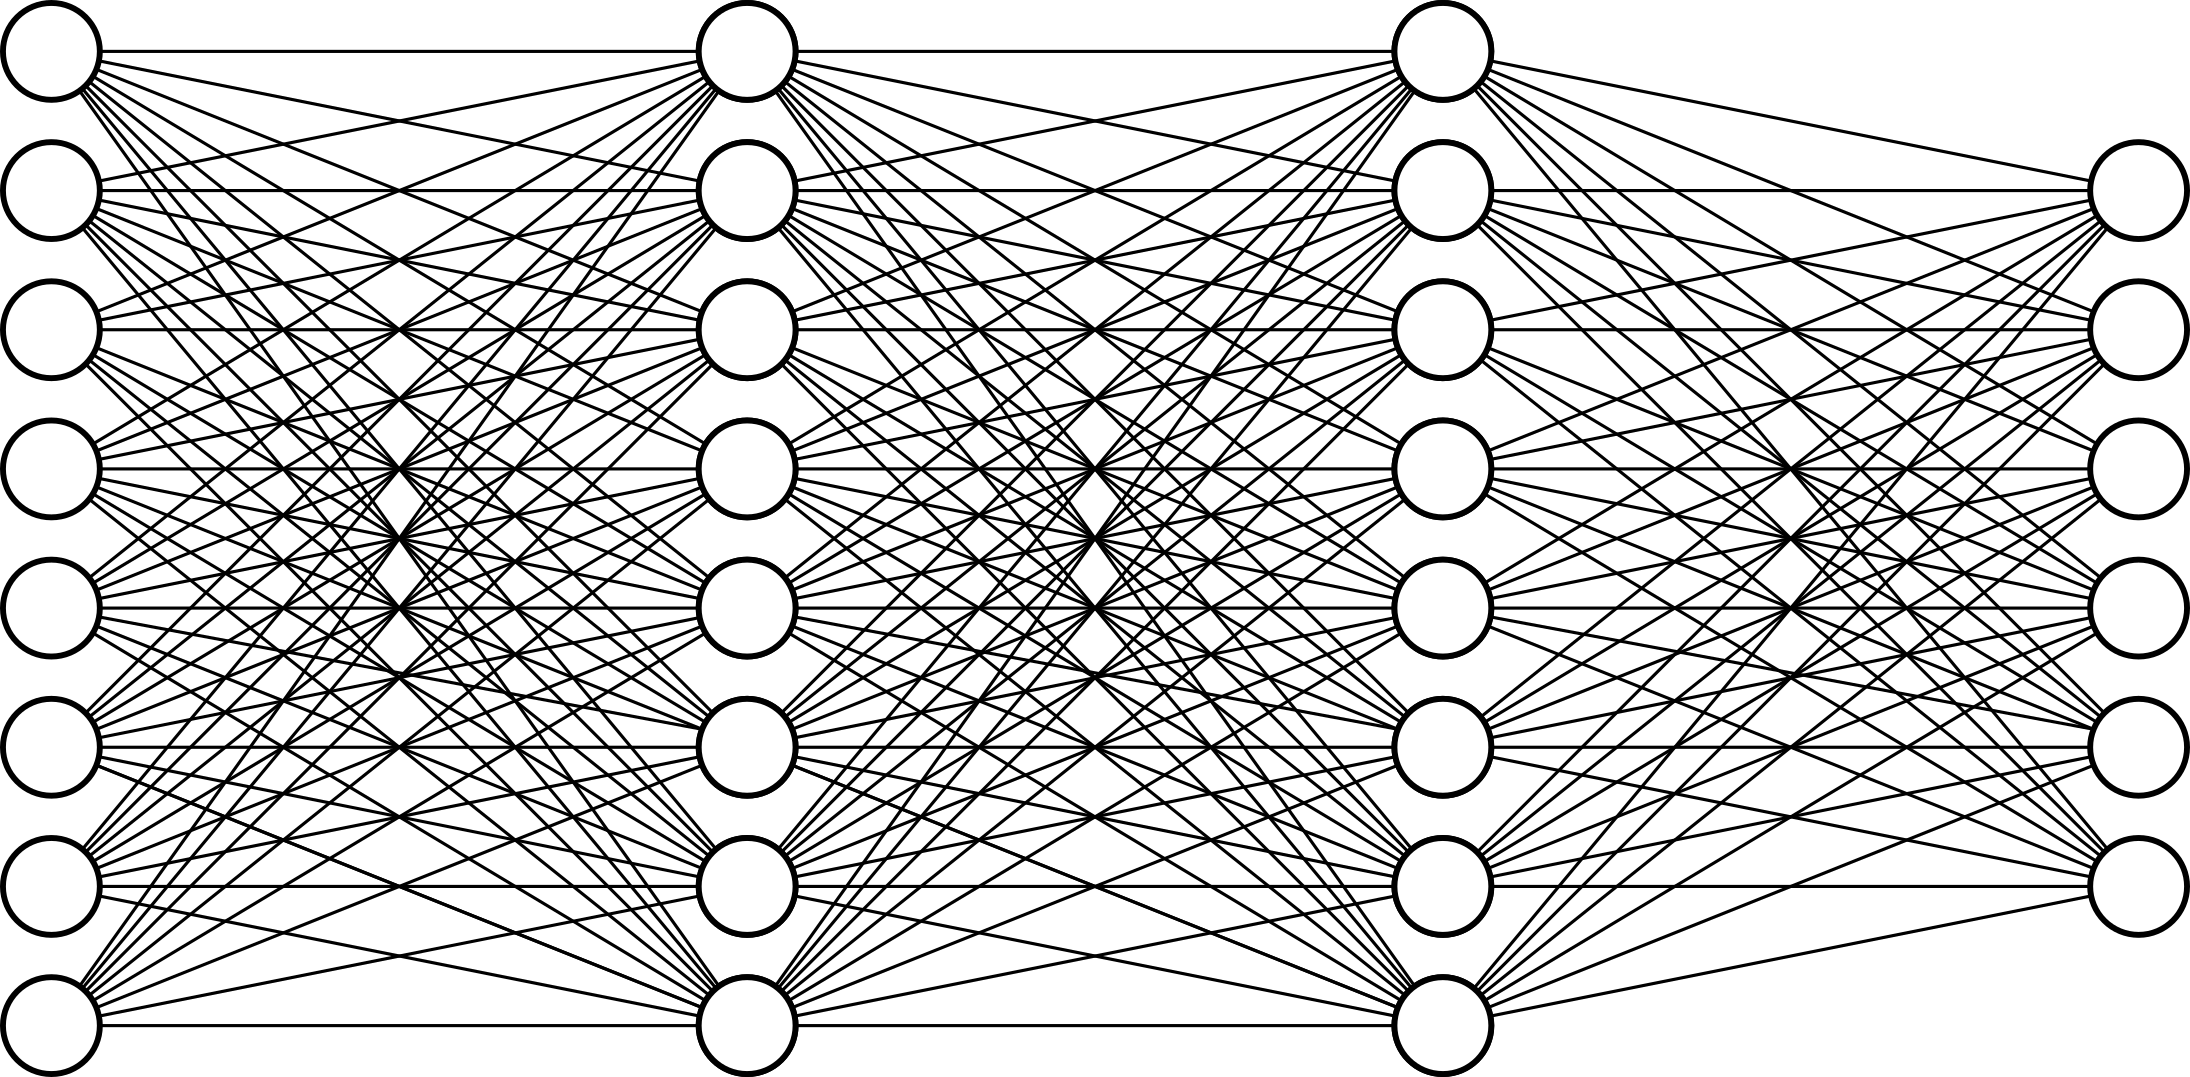
\includegraphics[height=3cm]{mini_reseau3_bis.png}
    \end{figure}
    \begin{figure}
      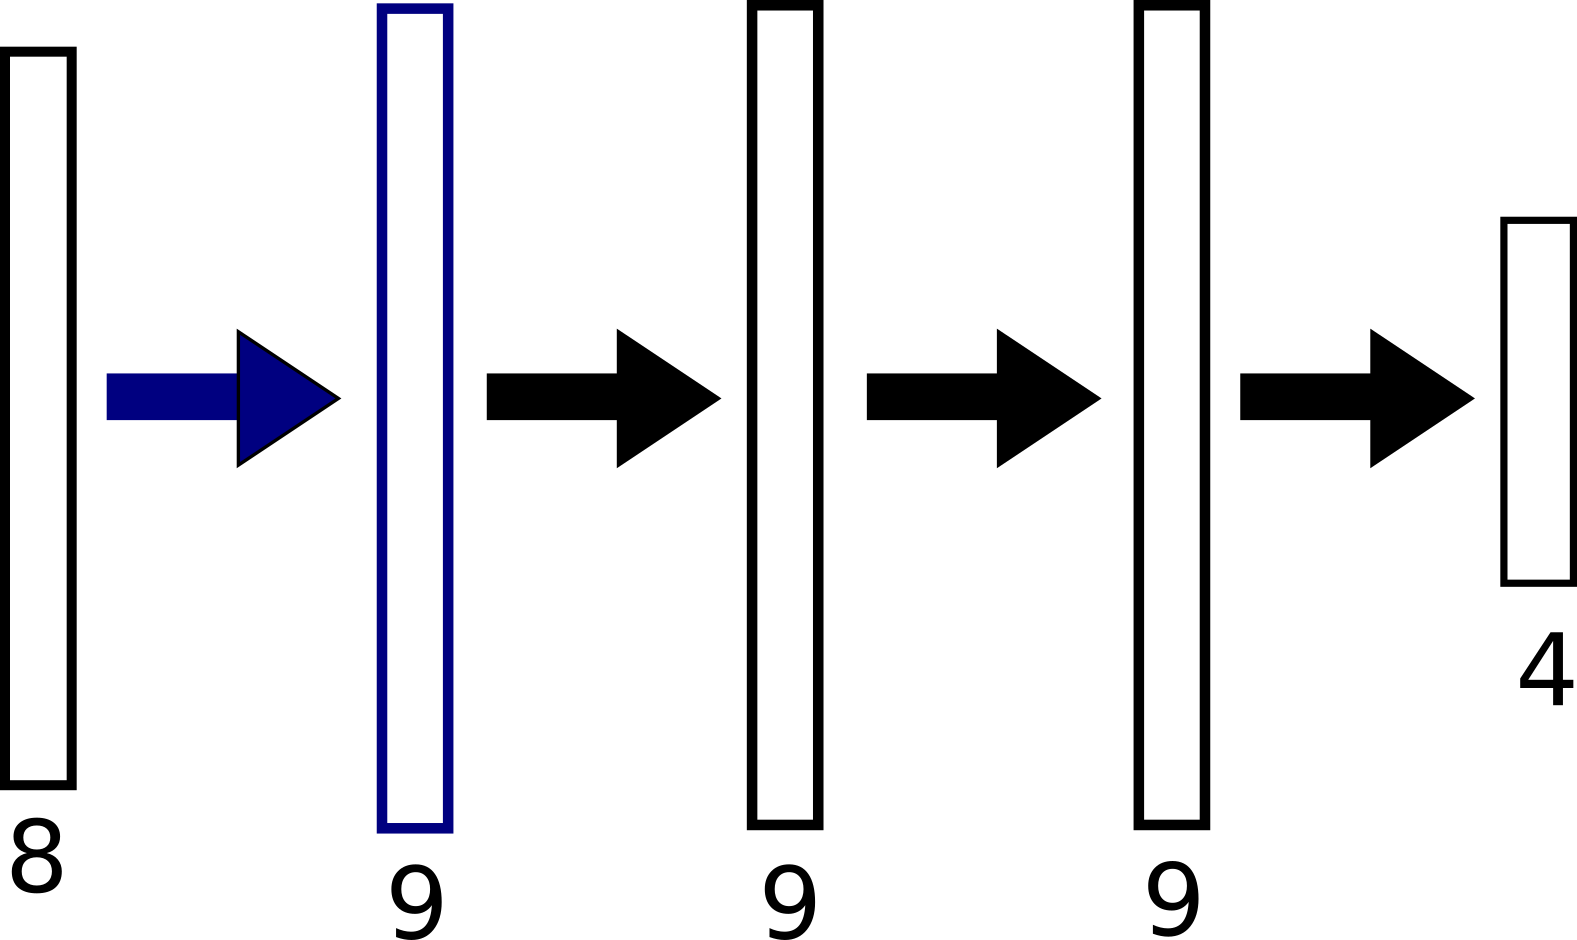
\includegraphics[height=3cm]{nn_representation}
    \end{figure}
  \end{column}

  \begin{column}{.5\textwidth}
    \begin{itemize}
    \item Data is organized into arrays, linked with operators
    \item A layer corresponds to an operator between arrays.
    \end{itemize}
  \end{column}
\end{columns}

\end{frame}


%%%%%%%%%%%%%%%%%%%%%%%%%%%%%%%%%%%%
%% \begin{frame}{The equations of fully-connected layers}

%%     \begin{figure}
%%       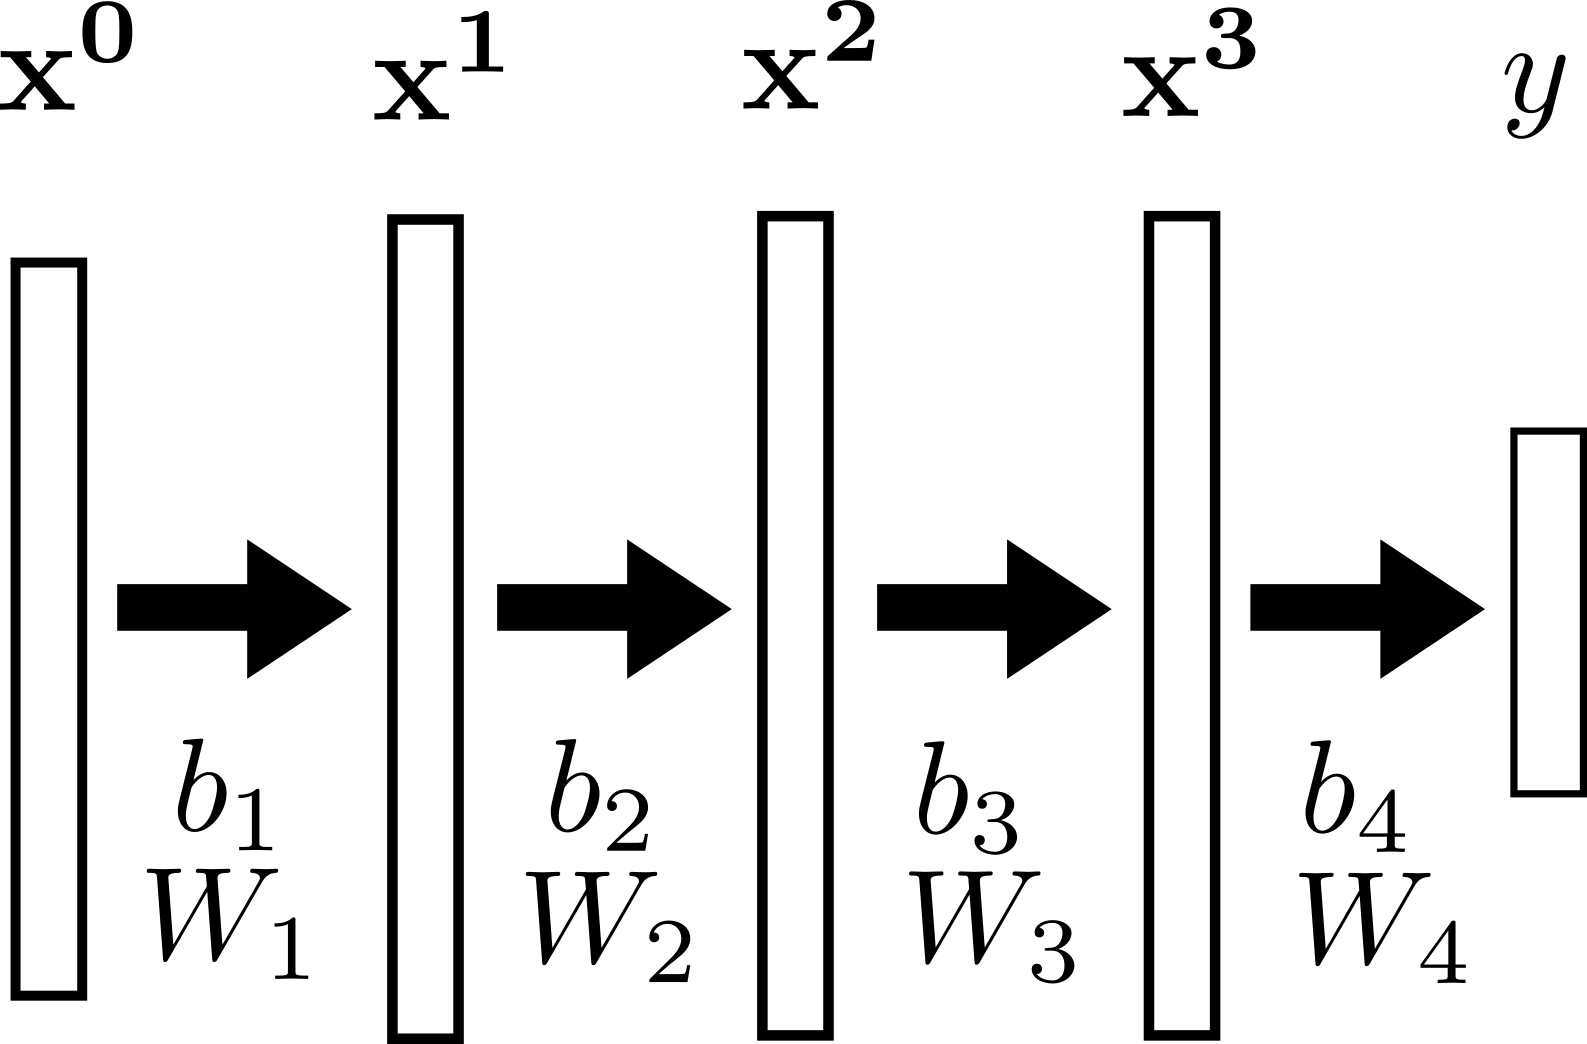
\includegraphics[height=3cm]{nn_representation2}
%%     \end{figure}

%%     \begin{block}{}
%%       \[\x^i = \act_i(\W_i\x^{i-1} + \bias_i),\, i= 1, 2, 3 \]
%%       \[y = \act_4(\W_4\x^4 + \bias_4)\]
%%     \end{block}

%% \end{frame}


%%%%%%%%%%%%%%%%%%%%%%%%%%%%%%%%%%%%%%%%%%%%%%%%%%
\section{Convolutional neural networks}
%%%%%%%%%%%%%%%%%%%%%%%%%%%%%%%%%%%%%%%%%%%%%%%%%%

%%%%%%%%%%%%%%%%%%%%%%%%%%%%%%%%%%%%%%%%%%%%%%%%%%
\begin{frame}{Machine Learning: basic definitions}
\begin{itemize}
	\item Machine Learning aims at predicting some output $y$ from an input (or measurement) $x$:
	\begin{equation}
	y = f(x)
	\end{equation}
	\item In this formulation, Machine Learning aims at finding (learning) $f$ from available data.
	\item The data that is used to learn $f$ is called \textbf{training set}, denoted by $\X$.
	\item In this general formulation, there is no particular limitation as to the mathematical nature of $x$ and $y$.
\end{itemize}
\end{frame}

\begin{frame}{A simple example: polynomial curve fitting\footnote{Example adapted from \cite{Bishop2006}}}
\begin{figure}[htb]
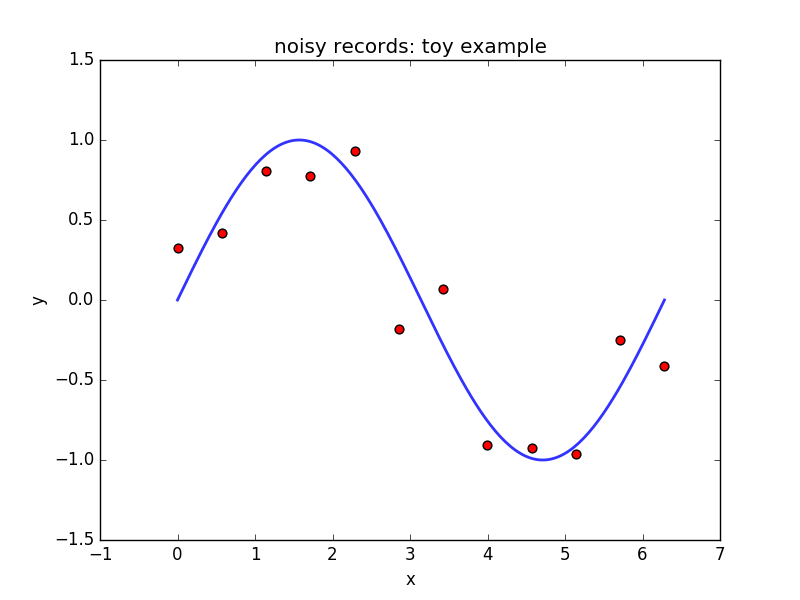
\includegraphics[width=0.6\textwidth]{../graphics/sample_from_sin.png}
\end{figure}
\begin{itemize}
	\item From a set of measured points $(x_i, y_i)$ (red), we would like to build a model to predict the value $y$ for any given $x$.
	\item The true function is $g(x)=\sin (x)$ (displayed in blue).
	\item The measurements $y_i$ are noisy outputs of that function, i.e.
	\begin{equation}
	y_i = \sin (x_i) + \epsilon \; , \;\;\; \;\;\; \epsilon \sim \mathcal{N}(0,0.2)
	\end{equation}
\end{itemize}
\end{frame}

\begin{frame}{A simple example: polynomial curve fitting}
\begin{itemize}
	\item We use the following polynomial model:
	\begin{eqnarray}
	f(x) &=& a_0 + a_1 x + a_2 x^2 + \ldots + a_m x^m \nonumber \\
	&=& \param^T \featmap (x)
	\end{eqnarray}
	\item Parameter vector: $\param = (a_0, a_1, \ldots, a_m)^T$
	\item Here, the initial measurement $x$ is a scalar. In our model, we map $x$ to a higher dimensional space:
	\begin{eqnarray}
		\featmap : \mathbb{R}^{\nfeatures} &\rightarrow & \mathbb{R}^Q \nonumber \\
		x &\rightarrow & \featmap (x) = (1, x, x^2, \ldots, x^m)^T
	\end{eqnarray}
	\item The model is linear in the parameters $\theta$ and linear in $\featmap$, but for $m>1$, the model is not linear in $x$.
\end{itemize}
\end{frame}

\begin{frame}{A simple example: polynomial curve fitting}
\begin{itemize}
	\item One classical approach is to minimize the least squared error between measured and predicted values:
	\begin{eqnarray}
		\min_{\param} \loss(\param) &=& \min_{\param} \sum_{i=1}^N (y_i - f(x_i))^2 \nonumber \\
		&=& \min_{\param} \sum_{i=1}^N (y_i - \param^T \featmap (x_i))^2
	\end{eqnarray}
	\item This can be achieved by setting the gradient with respect to $\param$ to zero:
	\begin{equation}
		\nabla_{\param} \loss = (\frac{\partial \loss}{\partial a_0}, \frac{\partial \loss}{\partial a_1}, \ldots, \frac{\partial \loss}{\partial a_m} )^T = 0
	\end{equation}
	\item Unlike most optimization problems in this course, this leads to an analytical solution for $\param$. This is known as \textbf{linear regression}. For more details, we refer to \cite{Hastie2009}.
\end{itemize}
\end{frame}

\begin{frame}{Overfitting and underfitting}
\begin{columns}
\begin{column}{.8\textwidth}
\begin{figure}[htb]
	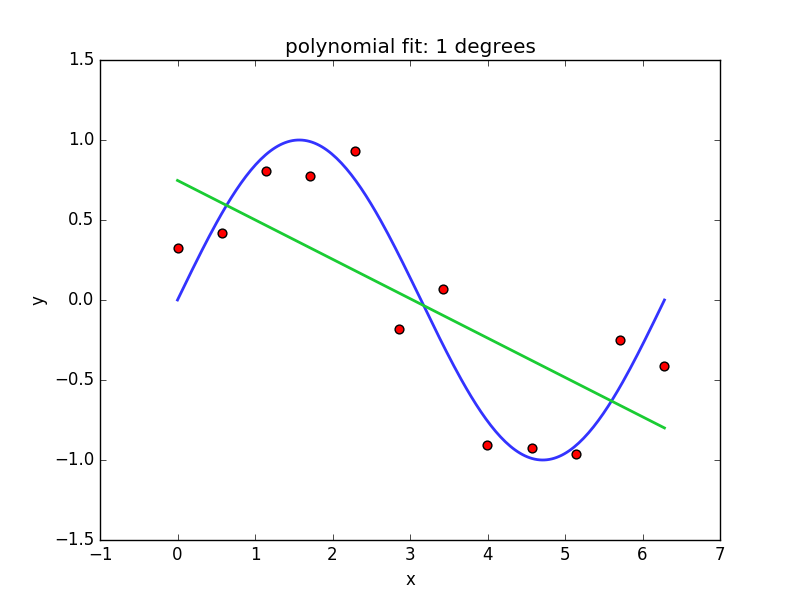
\includegraphics[width=0.75\textwidth]{../graphics/polyfit_degree_1.png}
\end{figure}
\end{column}
\begin{column}{.2\textwidth}
$\| \param \|^2 = 0.67$
\end{column}
\end{columns}
For $m=1$, the model is linear in its inputs. The solution is not capable of modeling the measured data points; we get a poor approximation of the original function. The family of functions we have used was not complex enough to model the true data distribution. We also speak of \textbf{underfitting}.
%\begin{textblock}{0}(.9\textwidth,\paperheight)
%  Test
% \end{textblock}
\end{frame}

\begin{frame}{Overfitting and underfitting}
\begin{columns}
\begin{column}{.8\textwidth}
\begin{figure}[htb]
	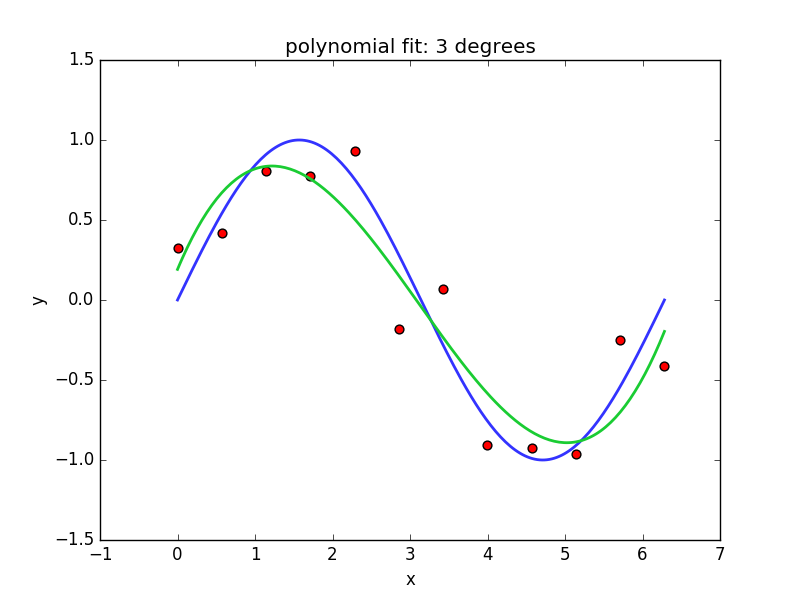
\includegraphics[width=0.75\textwidth]{../graphics/polyfit_degree_3.png}
\end{figure}
\end{column}
\begin{column}{.2\textwidth}
$\| \param \|^2 = 1.72$
\end{column}
\end{columns}
For $m=3$, we obtain a solution that seems to be quite right: it is sufficiently complex to model the true data distribution, but not too complex to model the small variations which are due to noise.
\end{frame}

\begin{frame}{Overfitting and underfitting}
\begin{columns}
\begin{column}{.8\textwidth}
\begin{figure}[htb]
	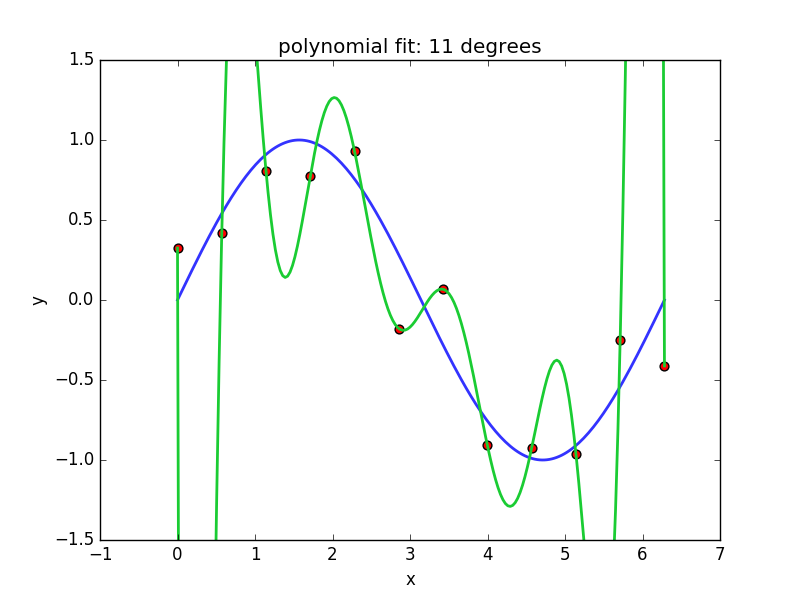
\includegraphics[width=0.75\textwidth]{../graphics/polyfit_degree_11.png}
\end{figure}
\end{column}
\begin{column}{.2\textwidth}
$\| \param \|^2 \approx 10^7$
\end{column}
\end{columns}
For $m=11$, we obtain a solution that has zero error (the function passes through every point of the training set). But the coefficients with large absolute values that cancel each other precisely on the training points lead to a highly unstable function. We speak of \textbf{overfitting} and \textbf{poor generalization}.
\end{frame}

\begin{frame}{Overfitting and underfitting}
\begin{columns}
\begin{column}{.8\textwidth}
\begin{figure}[htb]
	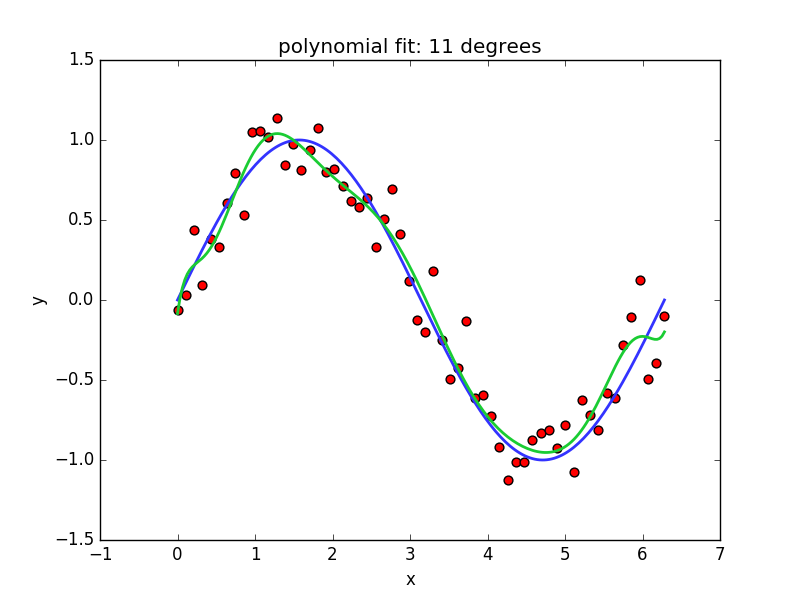
\includegraphics[width=0.75\textwidth]{../graphics/polyfit_degree_11_N60.png}
\end{figure}
\end{column}
\begin{column}{.2\textwidth}
$\| \param \|^2 = 5647$
\end{column}
\end{columns}
One way of reducing overfitting is to increase the number of samples. Even if the function is complex, it cannot be “too wild”, as it has to find a compromise between many training samples. This however implies the annotation (or measurement) of more samples.
\end{frame}

\begin{frame}{Overfitting and underfitting}
\begin{columns}
\begin{column}{.8\textwidth}
\begin{figure}[htb]
	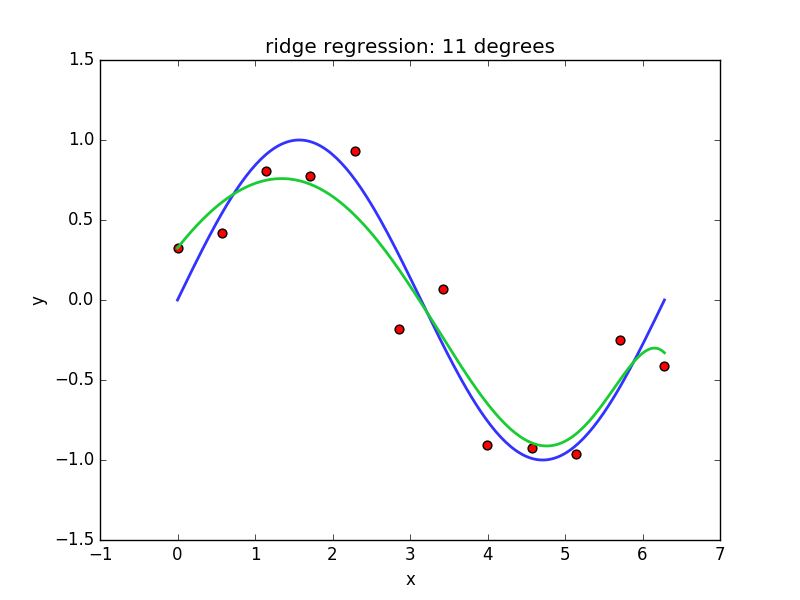
\includegraphics[width=0.75\textwidth]{../graphics/ridge_regression_11_10.png}
\end{figure}
\end{column}
\begin{column}{.2\textwidth}
$\| \param \|^2 = 0.41$
\end{column}
\end{columns}
Another way of preventing overfitting without increasing the number of samples, is to add a penalization term in the optimization procedure. This is also known as \textbf{regularization}:
\begin{equation}
	\loss = \sum_{i=1}^N (y_i - \param^T \featmap (x_i))^2 + \lambda \| \param \|^2
\end{equation}
\end{frame}


%%%%%%%%%%%%%%%%%%%%%%%%%%%%%%%%%%%%
\begin{frame}{A picture is worth a thousand words}

  \begin{columns}
    \begin{column}{.5\textwidth}
      \begin{block}{Definition}
        \begin{itemize}
        \item Classically, an image is a matrix of values belonging to $[0, \ldots, 255]$ (grey level images) or to $[0, \ldots, 255]^3$ (color images).
        \item More generally, an image is a $q$-dimensional array of values belonging to $R^d$.
        \end{itemize}
      \end{block}

    \end{column}

    \begin{column}{.5\textwidth}
      \begin{figure}
        \centering
        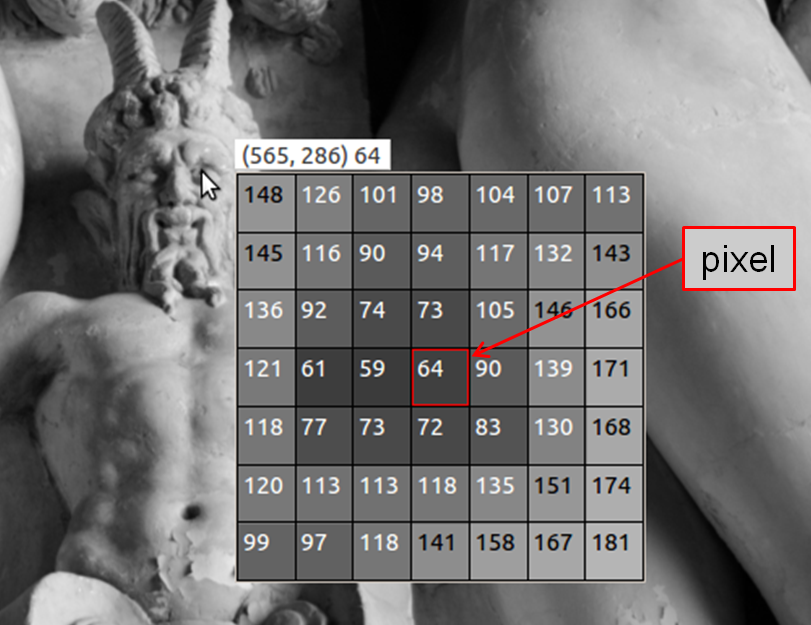
\includegraphics[width=5cm]{faune.png}\\
        \tiny{Grey level values around the left eye of the faun}
      \end{figure}

    \end{column}
  \end{columns}

\end{frame}


%%%%%%%%%%%%%%%%%%%%%%%%%%%%%%%%%%%%
\begin{frame}{The role of annotated image databases}

  Image databases including \emph{annotations} (typically some kind of high level information) are essential to the development of \emph{supervised} machine learning methods for image analysis.

  \begin{block}{Annotations}
    \begin{itemize}
    \item Image class
    \item Measure(s) obtained from the image
    \item Position of objects within the image
    \item Segmentation
    \end{itemize}
  \end{block}

\end{frame}

%%%%%%%%%%%%%%%%%%%%%%%%%%%%%%%%%%%%
%% \begin{frame}{MNIST database \tiny{\cite{lecun_gradient-based_1998}}}

%%   \begin{itemize}
%%   \item The Modified National Institute of Standards and Technology (MNIST) database contains $60\,000$ training images of hand-written digits, and $10,000$ test images.
%%   \item Image size: $28 \times 28$
%%   \item It has been used since 1998
%%   \item Human performance on a similar database (NIST) is reported to be around $1.5\%$ error \cite{simard_efficient_1993}
%%   \item Best methods, based on convolutional neural networks, give around $0.21\%$ test error.
%%   \end{itemize}

%% \end{frame}

%% %%%%%%%%%%%%%%%%%%%%%%%%%%%%%%%%%%%%
%% \begin{frame}{MNIST database}

%%   \centering
%%   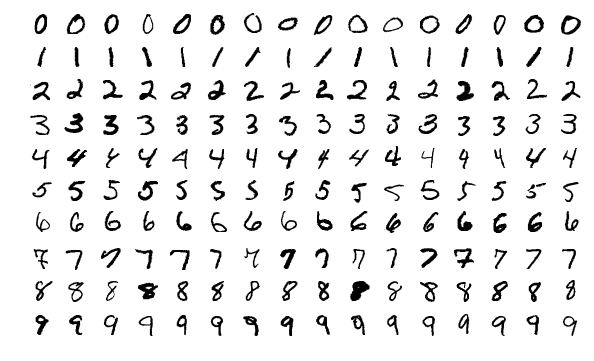
\includegraphics[width=\textwidth]{mnist_examples.png}\\
%%   \source{Images from MNIST assembled by Josef Stepan (licensed under CC BY-SA 4.0)}


%% \end{frame}



%%%%%%%%%%%%%%%%%%%%%%%%%%%%%%%%%%%%
\begin{frame}{Layers representation}

  \begin{block}{}
    For illustration purposes, in the following slides images and filters will be displayed as rows of neurons -- these can be seen as 1D arrays or as sections of 2D arrays.

    We represent some connections between neurons. Each such connection is associated to a weight. The bias are not represented, to avoid clutter, but must not be forgotten.
  \end{block}

  \begin{columns}

    \begin{column}<1->{0.33\textwidth}
      \begin{center}
        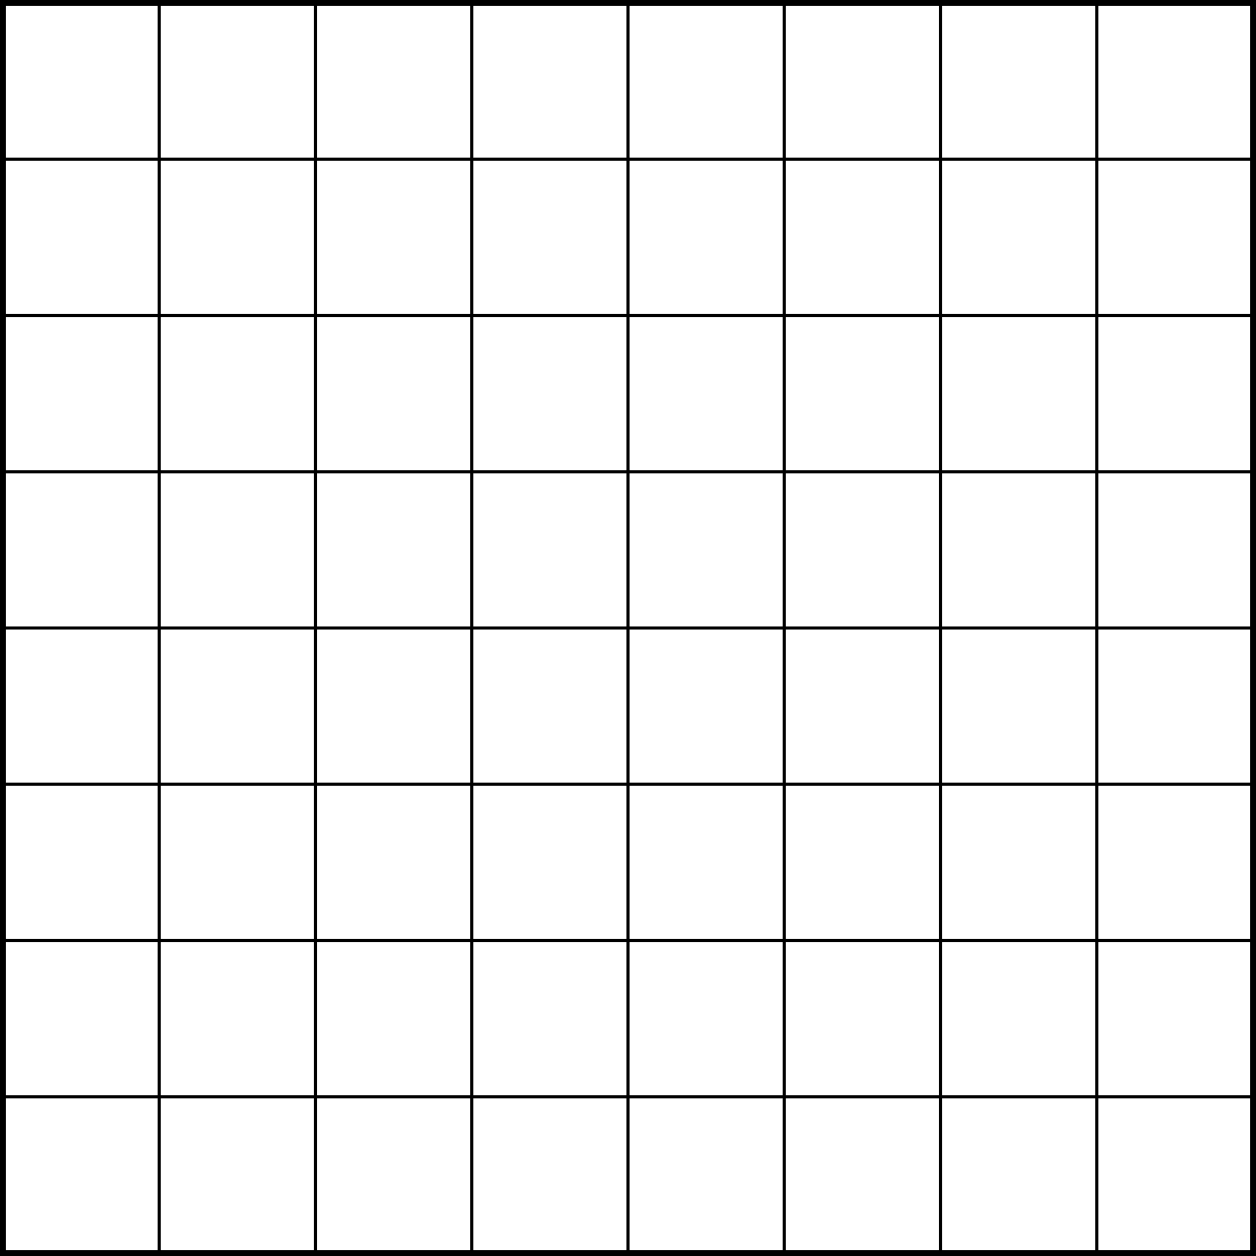
\includegraphics[width=0.80\textwidth]{cnn_pixels.png}
      \end{center}
    \end{column}

    \begin{column}<2->{0.33\textwidth}
      \begin{center}
        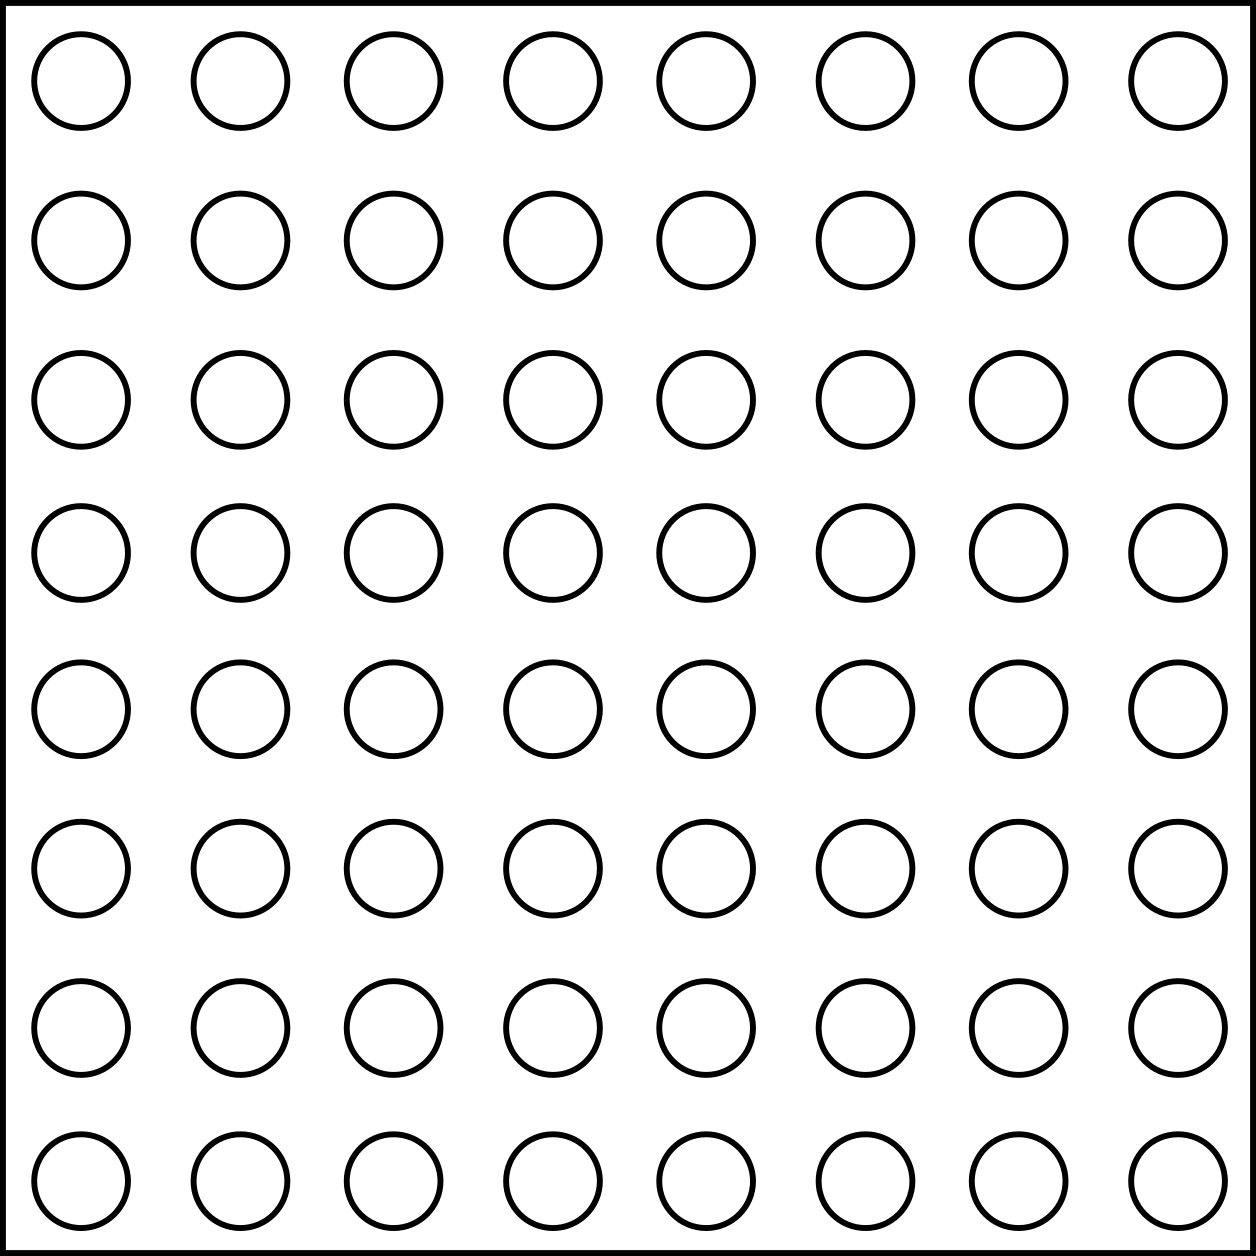
\includegraphics[width=0.80\textwidth]{cnn_neurones.png}

      \end{center}
    \end{column}

    \begin{column}<3->{0.33\textwidth}
      \begin{center}
        
\includegraphics[width=0.07\textwidth]{col.png}

      \end{center}
    \end{column}

  \end{columns}


\end{frame}


%%%%%%%%%%%%%%%%%%%%%%%%%%%%%%%%%%%%%%%%%%%%%%%%%%
\frame{
  \frametitle{Towards convolutional layers}


  \begin{columns}

    \begin{column}<1->{0.3\textwidth}
      \begin{center}
        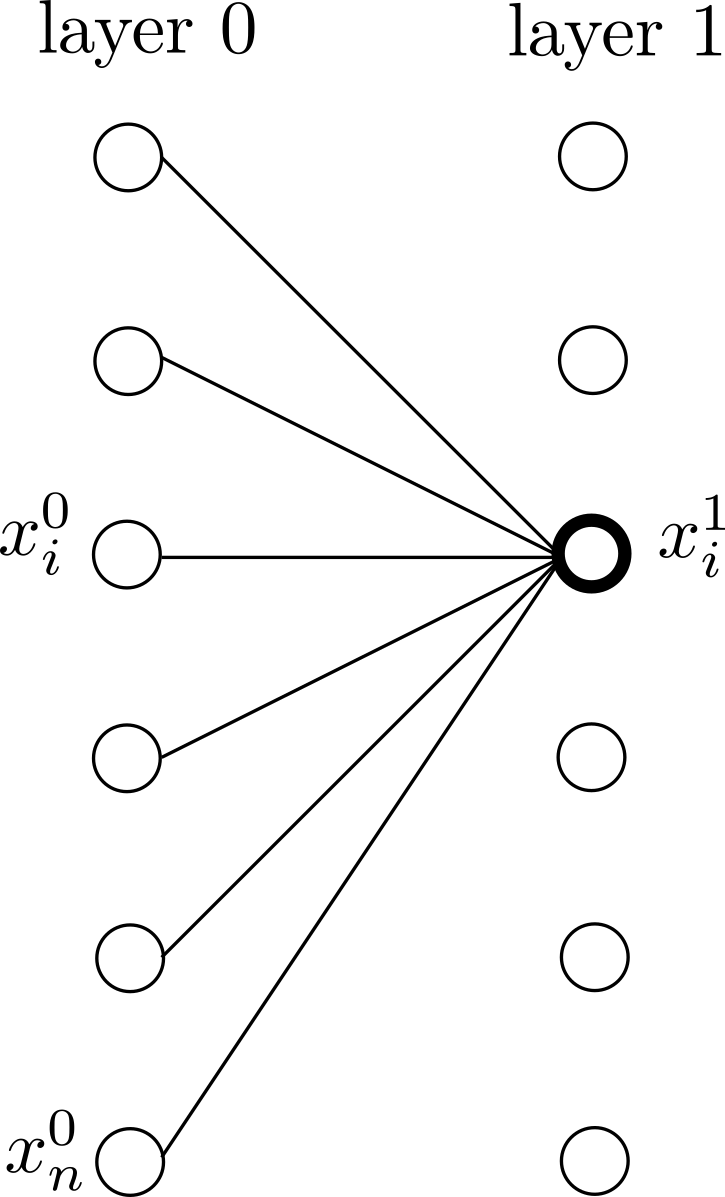
\includegraphics[width=0.74\textwidth]{fully_connected_layer.png}
        \\ \scriptsize{Fully connected layer: $n(n+1)$ weights}
      \end{center}
    \end{column}

    \begin{column}<2->{0.3\textwidth}
      \begin{center}
        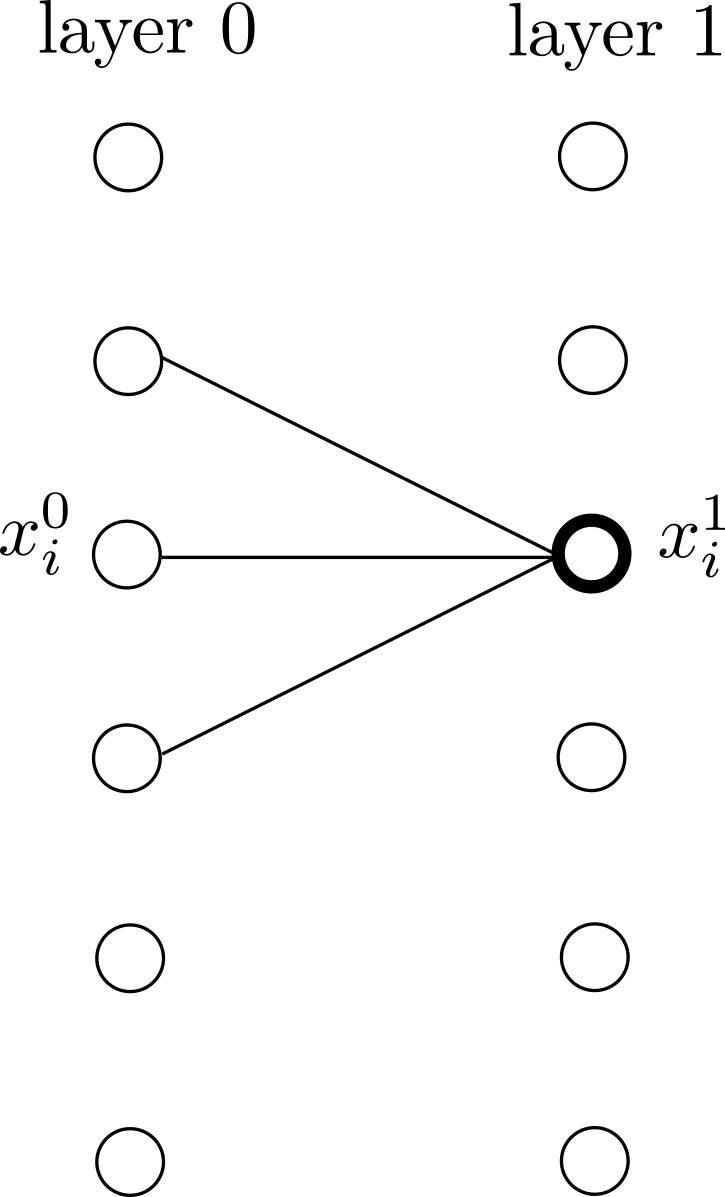
\includegraphics[width=0.74\textwidth]{locally_connected_layer.png}
        \\ \scriptsize{Locally conn. layer: $n(s+1)$ weights}
      \end{center}
    \end{column}

    \begin{column}<3->{0.3\textwidth}
      \begin{center}
        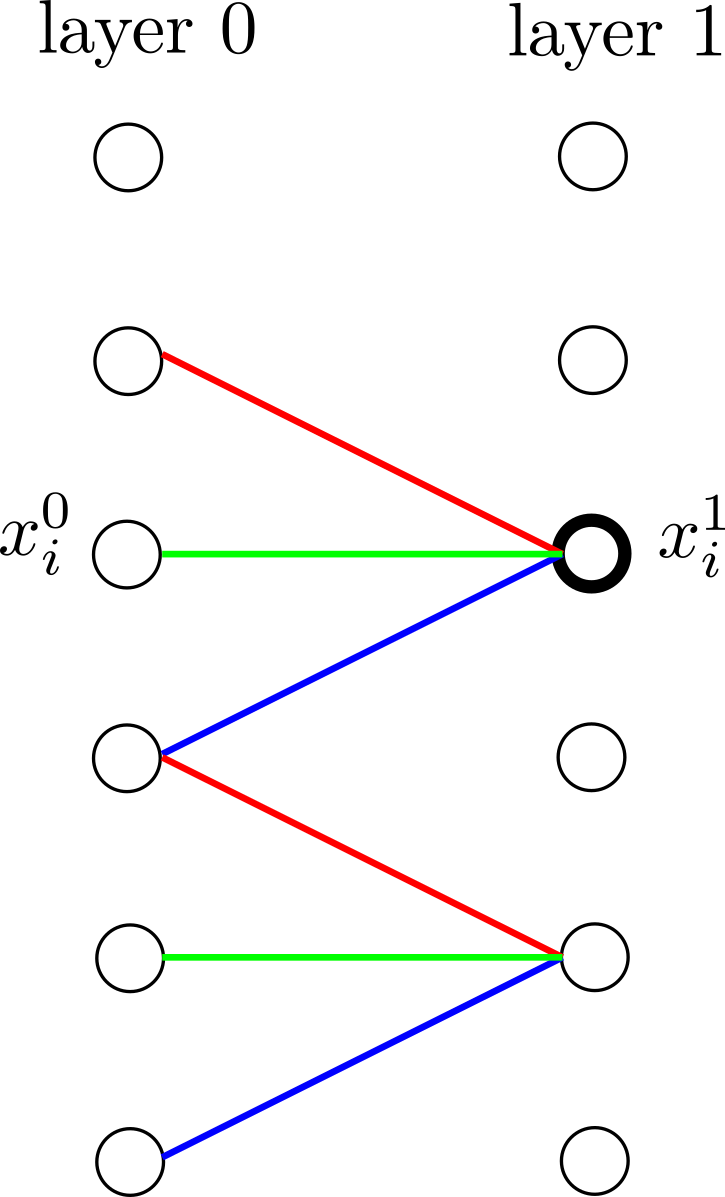
\includegraphics[width=0.74\textwidth]{convolutional_layer.png}
        \\ \scriptsize{Weight replication: $s+1$ weights.\\
          \alert{Convolutional layer.}}
      \end{center}
    \end{column}

  \end{columns}

}


%%%%%%%%%%%%%%%%%%%%%%%%%%%%%%%%%%%%%%%%%%%%%%%%%%
\frame{
  \frametitle{Towards convolutional layers: some figures}

  \begin{itemize}
  \item $3 \times 3$ convolutions: $s=9$
  \item \textcolor{blue}{Toy image: $n = 28 \times 28 = 784$}
  \item \textcolor{orange}{Typical image: $n = 1000 \times 1000 = 10^6$}
  \end{itemize}

  \begin{columns}

    \begin{column}{0.3\textwidth}
      \begin{center}
        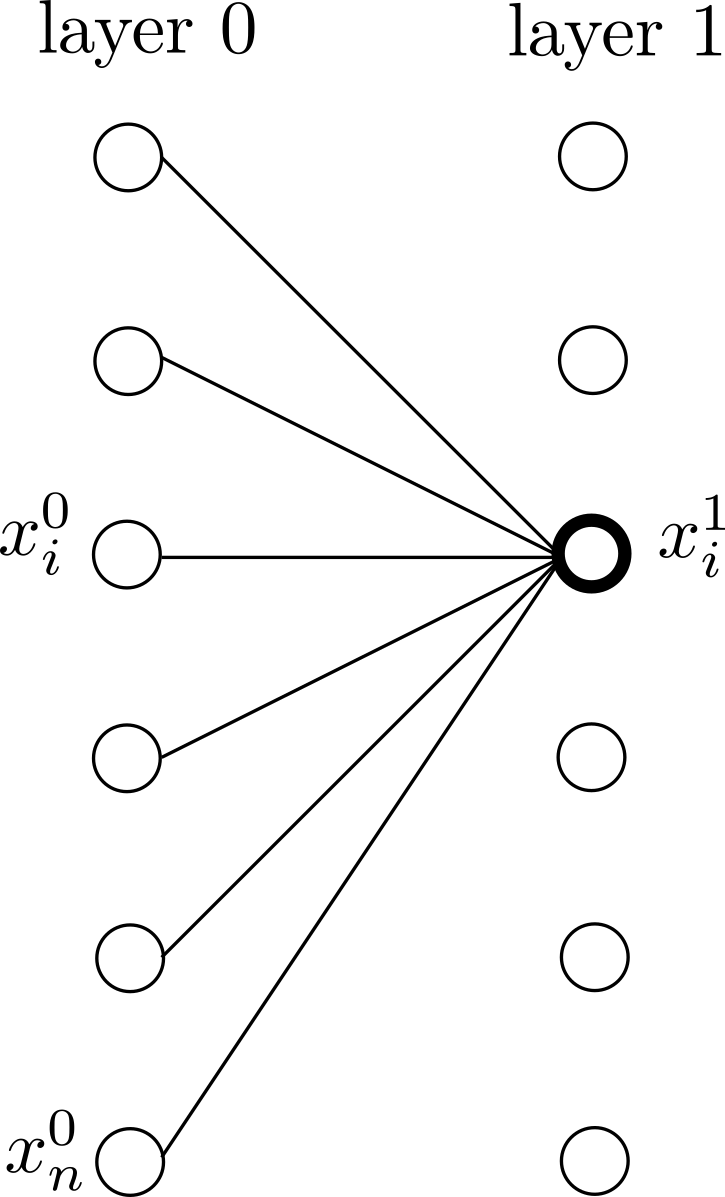
\includegraphics[width=0.74\textwidth]{fully_connected_layer.png}
        \\ \scriptsize{Fully connected layer: $n(n+1)$ weights}
        \\ \textcolor{blue}{\scriptsize{$\approx 6.10^5$}}
        \\ \textcolor{orange}{\scriptsize{$\approx 10^{12}$}}
      \end{center}
    \end{column}

    \begin{column}{0.3\textwidth}
      \begin{center}
        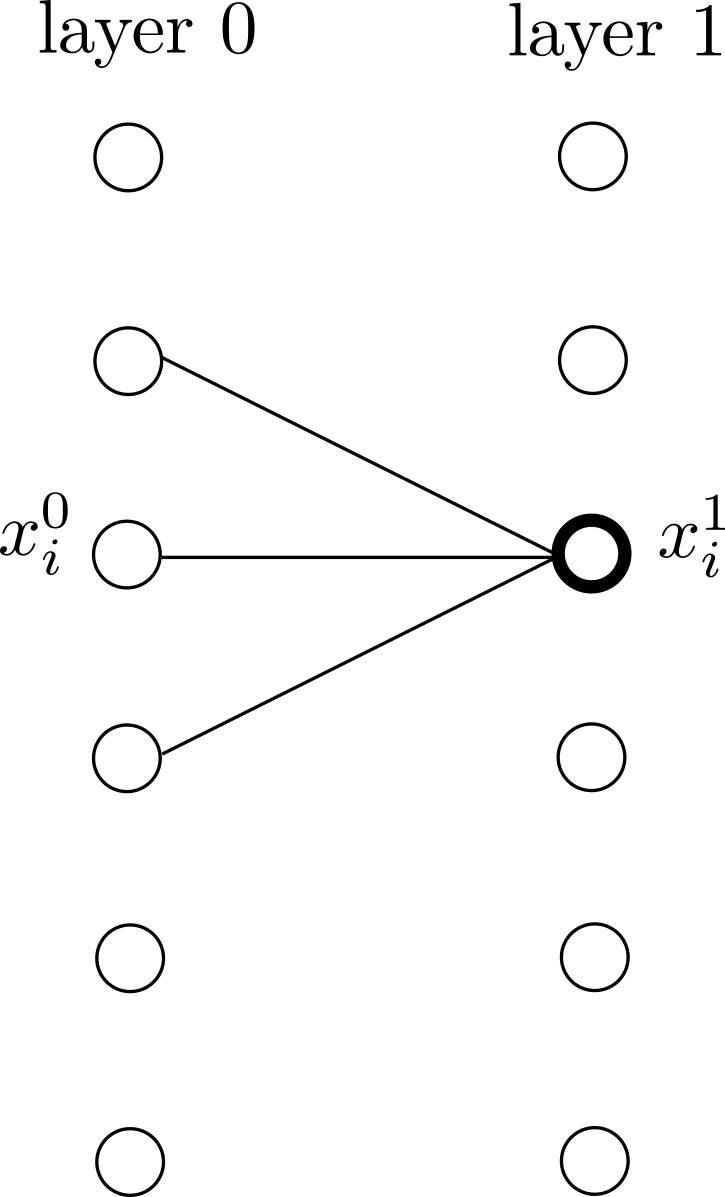
\includegraphics[width=0.74\textwidth]{locally_connected_layer.png}
        \\ \scriptsize{Locally conn. layer: $n(s+1)$ weights}
        \\ \textcolor{blue}{\scriptsize{$7840$}}
        \\ \textcolor{orange}{\scriptsize{$10^7$}}
      \end{center}
    \end{column}

    \begin{column}{0.3\textwidth}
      \begin{center}
        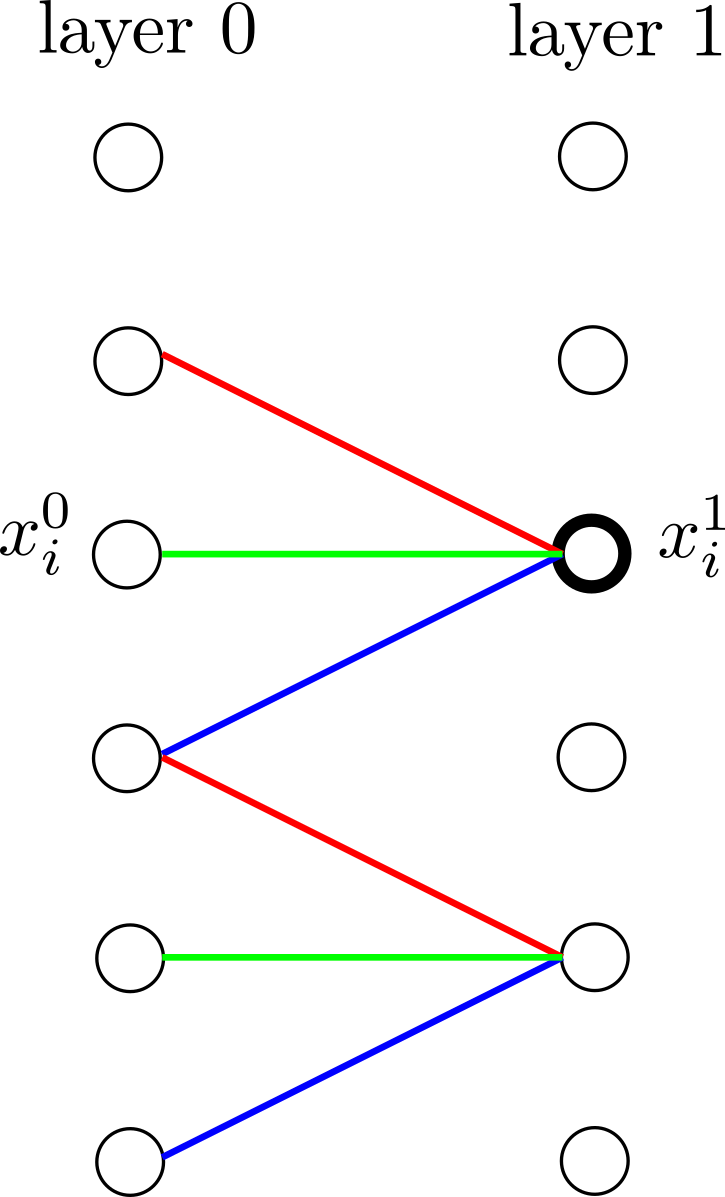
\includegraphics[width=0.74\textwidth]{convolutional_layer.png}
        \\ \scriptsize{Weight replication: $s+1$ weights.}
        \\ \textcolor{blue}{\scriptsize{$10$}}
        \\ \textcolor{orange}{\scriptsize{$10$}}

      \end{center}
    \end{column}

  \end{columns}
}


%%%%%%%%%%%%%%%%%%%%%%%%%%%%%%%%%%%%
\begin{frame}{Convolutional layer illustration in 2D}


  \begin{itemize}
  \item Illustration of a convolution of size $3 \times 3$
  \end{itemize}

  \begin{center}
    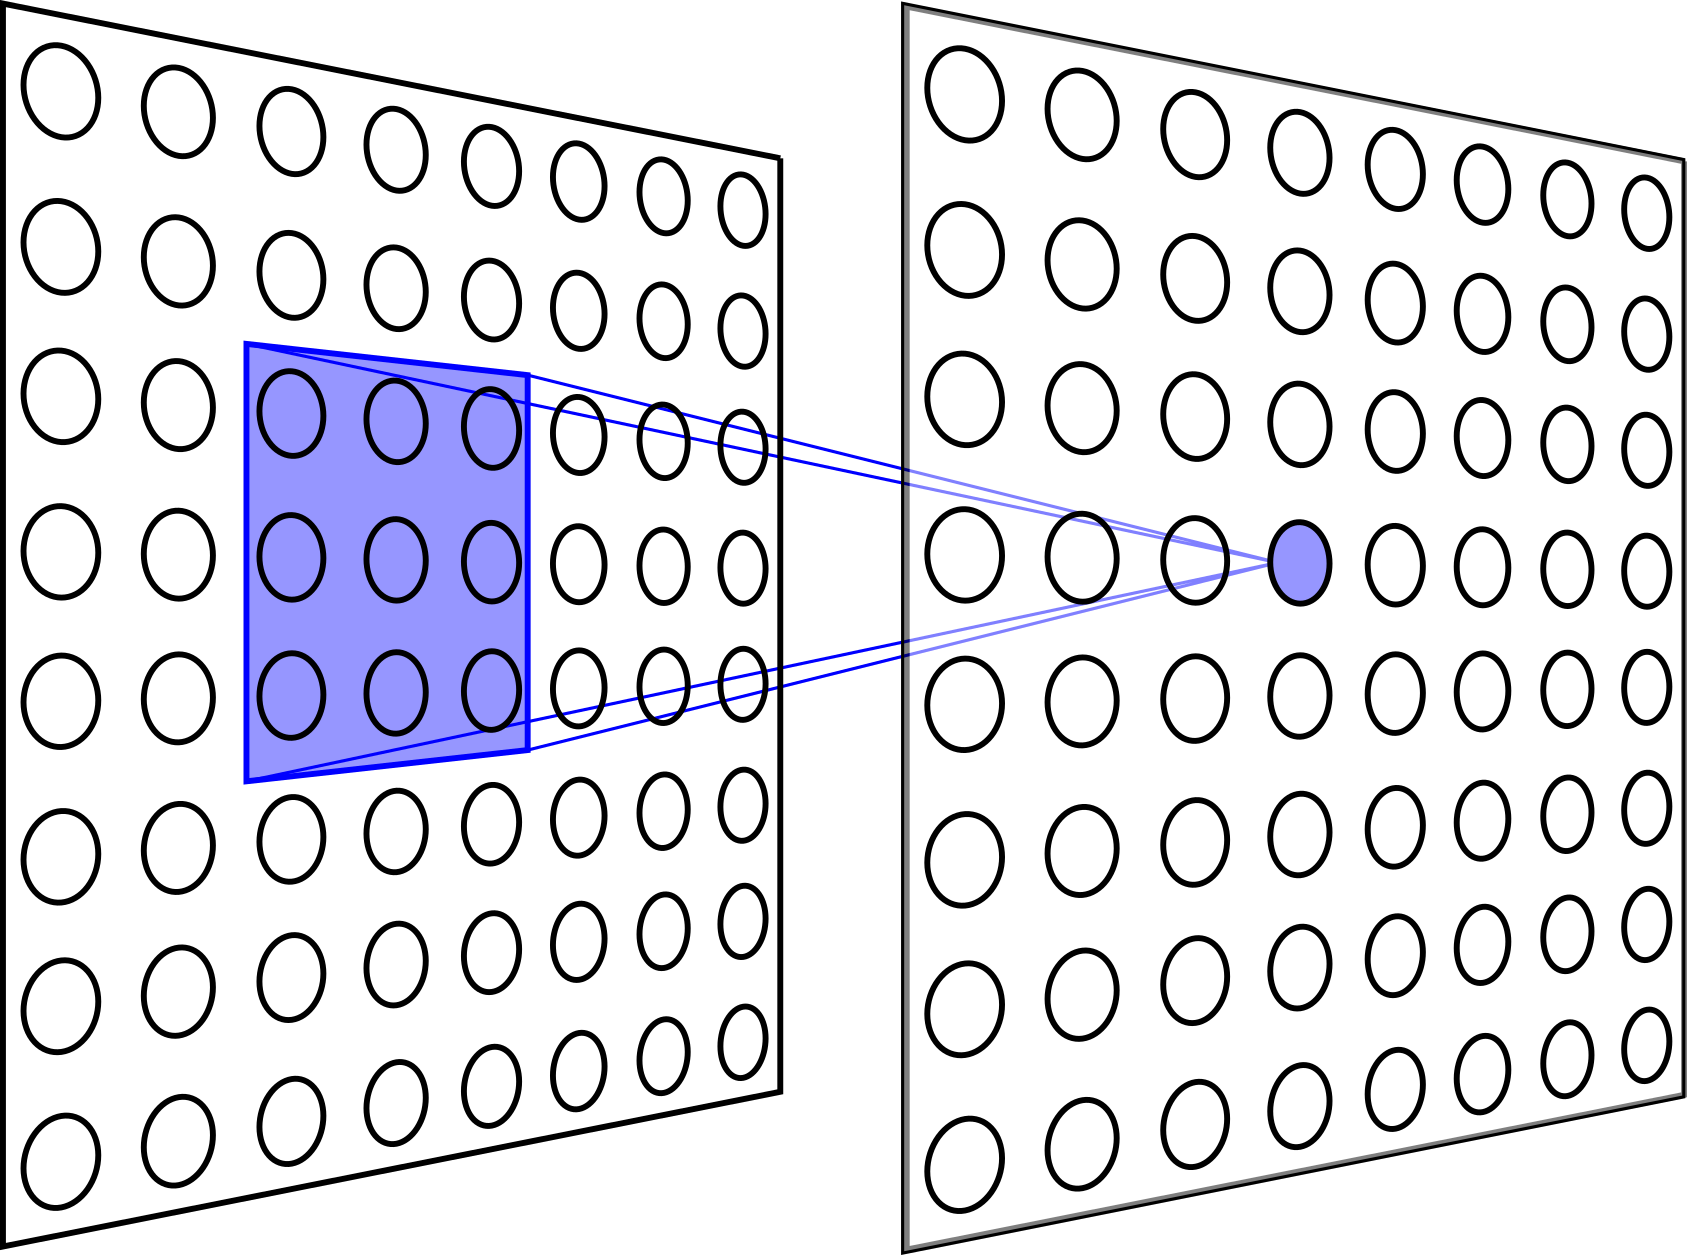
\includegraphics[width=0.5\textwidth]{cnn_complet}
  \end{center}


\end{frame}

%%%%%%%%%%%%%%%%%%%%%%%%%%%%%%%%%%%%%%%%%%%%%%%%%%
\frame{
  \frametitle{Stride}

  A convolutional layer can at the same time downsample the image by applying a sampling step, or \emph{stride}.

  \begin{columns}

    \begin{column}<1->{0.3\textwidth}
      \begin{center}
        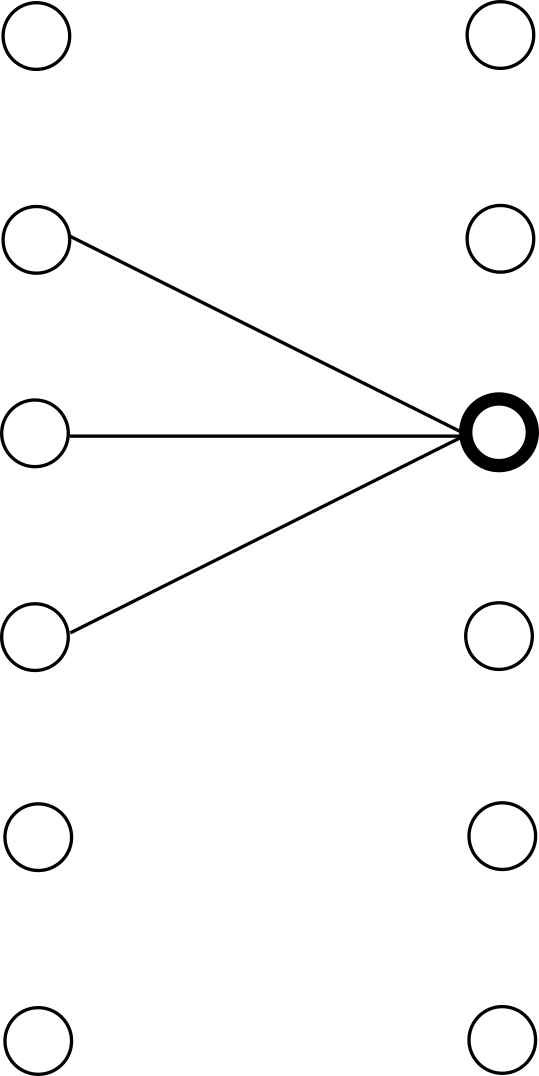
\includegraphics[width=0.60\textwidth]{stride1.png}
        \\ \scriptsize{Stride 1}
      \end{center}
    \end{column}

    \begin{column}<2->{0.3\textwidth}
      \begin{center}
        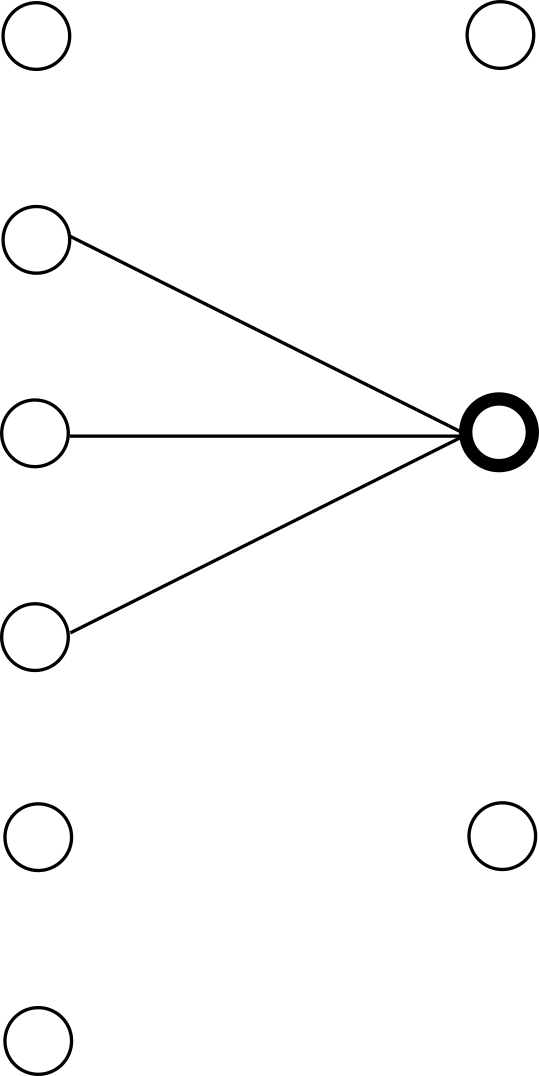
\includegraphics[width=0.60\textwidth]{stride2.png}
        \\ \scriptsize{Stride 2}
      \end{center}
    \end{column}

    \begin{column}<3>{0.3\textwidth}
      \begin{center}
        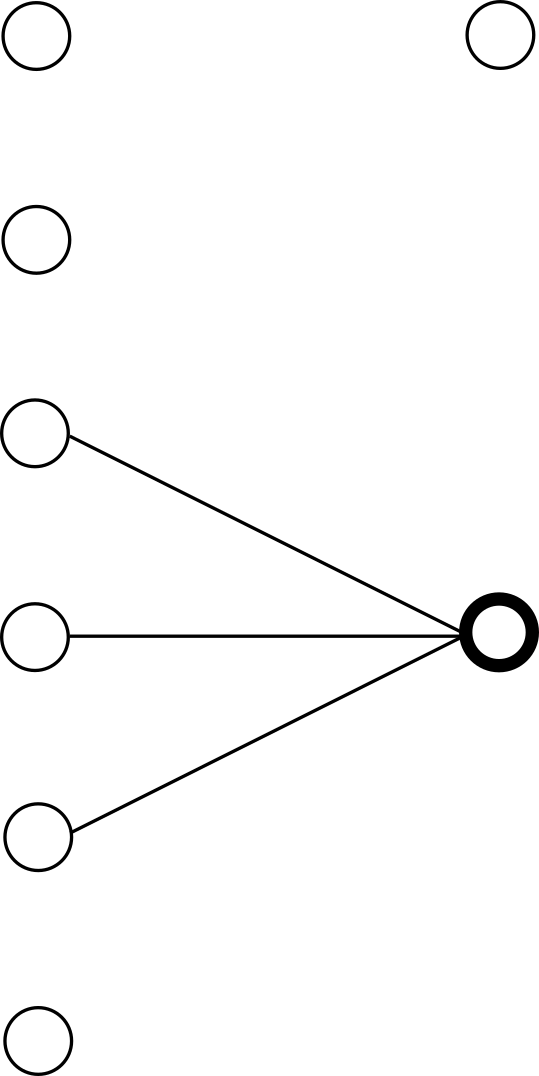
\includegraphics[width=0.60\textwidth]{stride3.png}
        \\ \scriptsize{Stride 3}
      \end{center}
    \end{column}

  \end{columns}

}

%%%%%%%%%%%%%%%%%%%%%%%%%%%%%%%%%%%%%%%%%%%%%%%%%%
\frame{
  \frametitle{Several filters in the same convolutional layer}


\begin{columns}
  \begin{column}{.53\textwidth}
  \begin{center}
    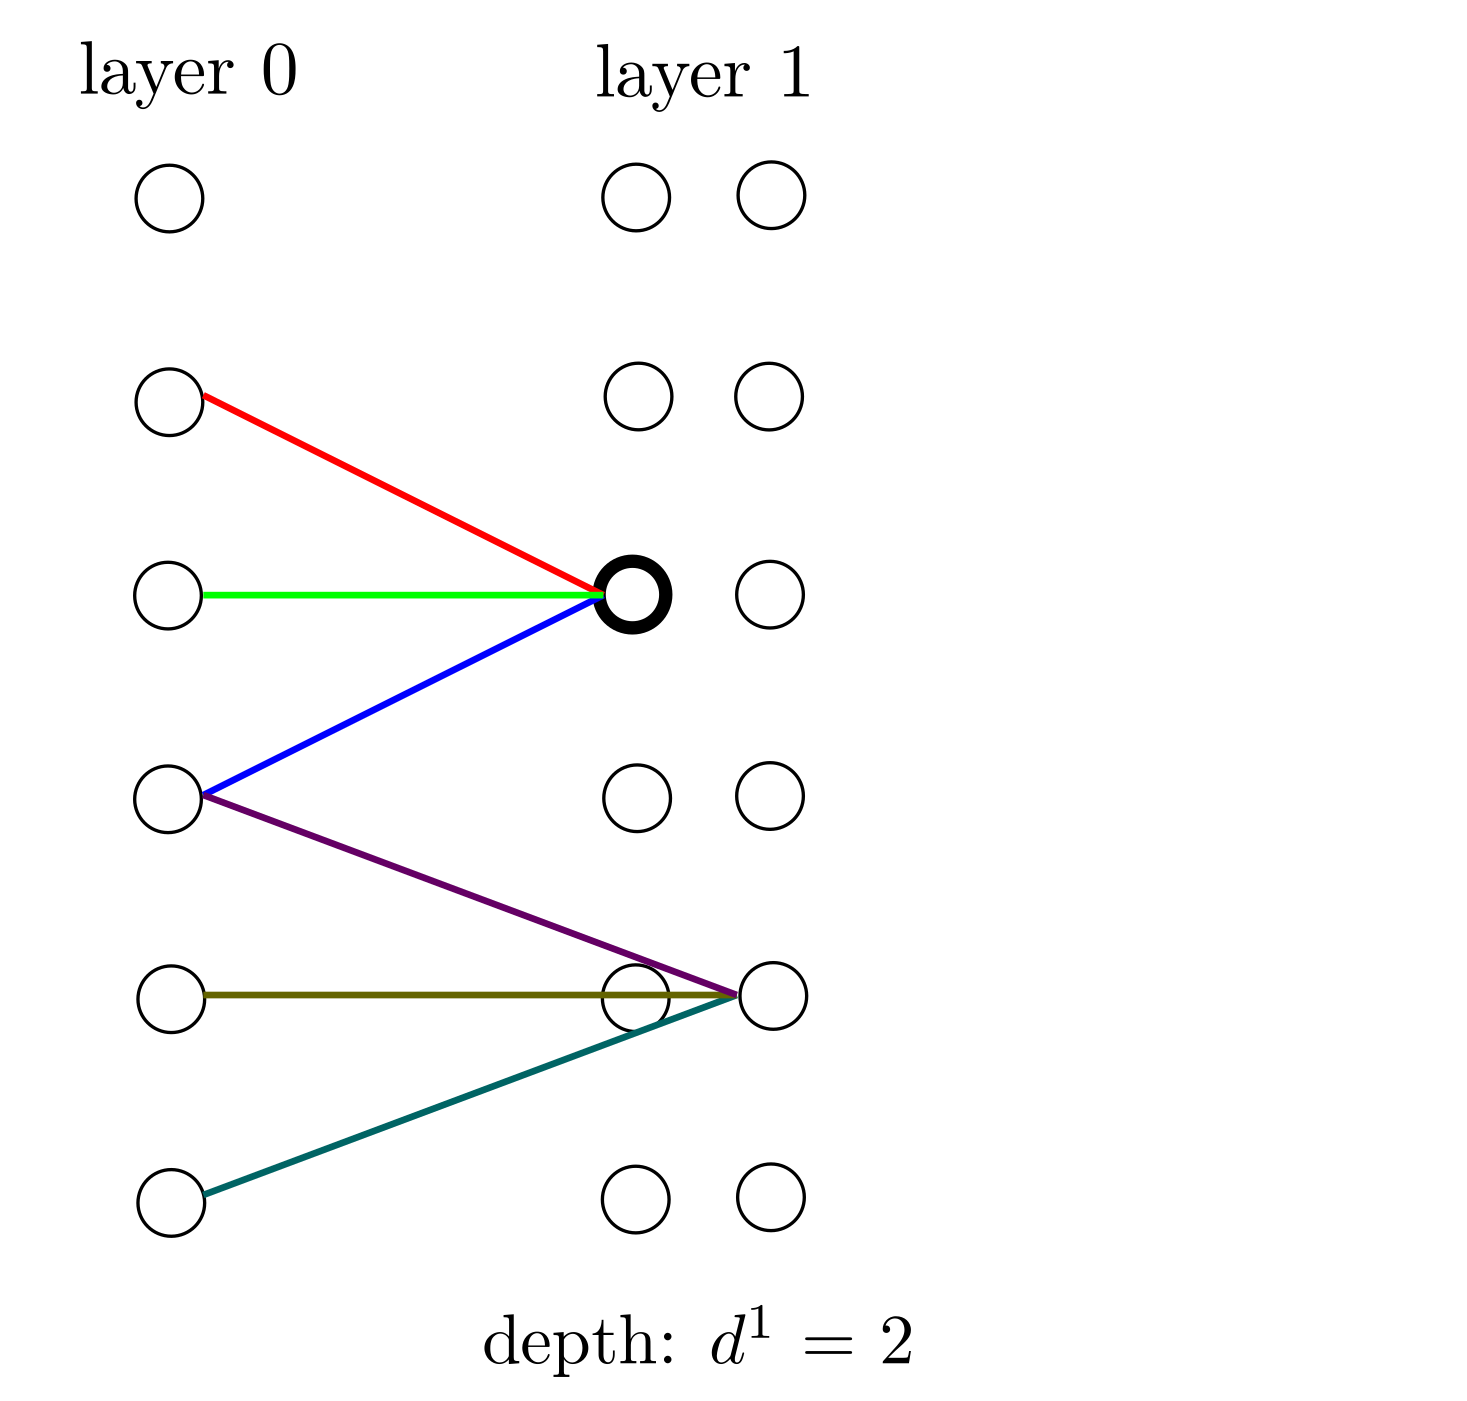
\includegraphics[width=\textwidth]{convolutional_layer2.png}
  \end{center}

  \end{column}

  \begin{column}{.47\textwidth}
\begin{block}{Note on vocabulary}
  The depth of a layer is often called the \alert{number of filters}.
\end{block}
  \end{column}
\end{columns}



}

%%%%%%%%%%%%%%%%%%%%%%%%%%%%%%%%%%%%%%%%%%%%%%%%%%
\frame{
  \frametitle{Several filters in the same convolutional layer}

  \begin{center}
    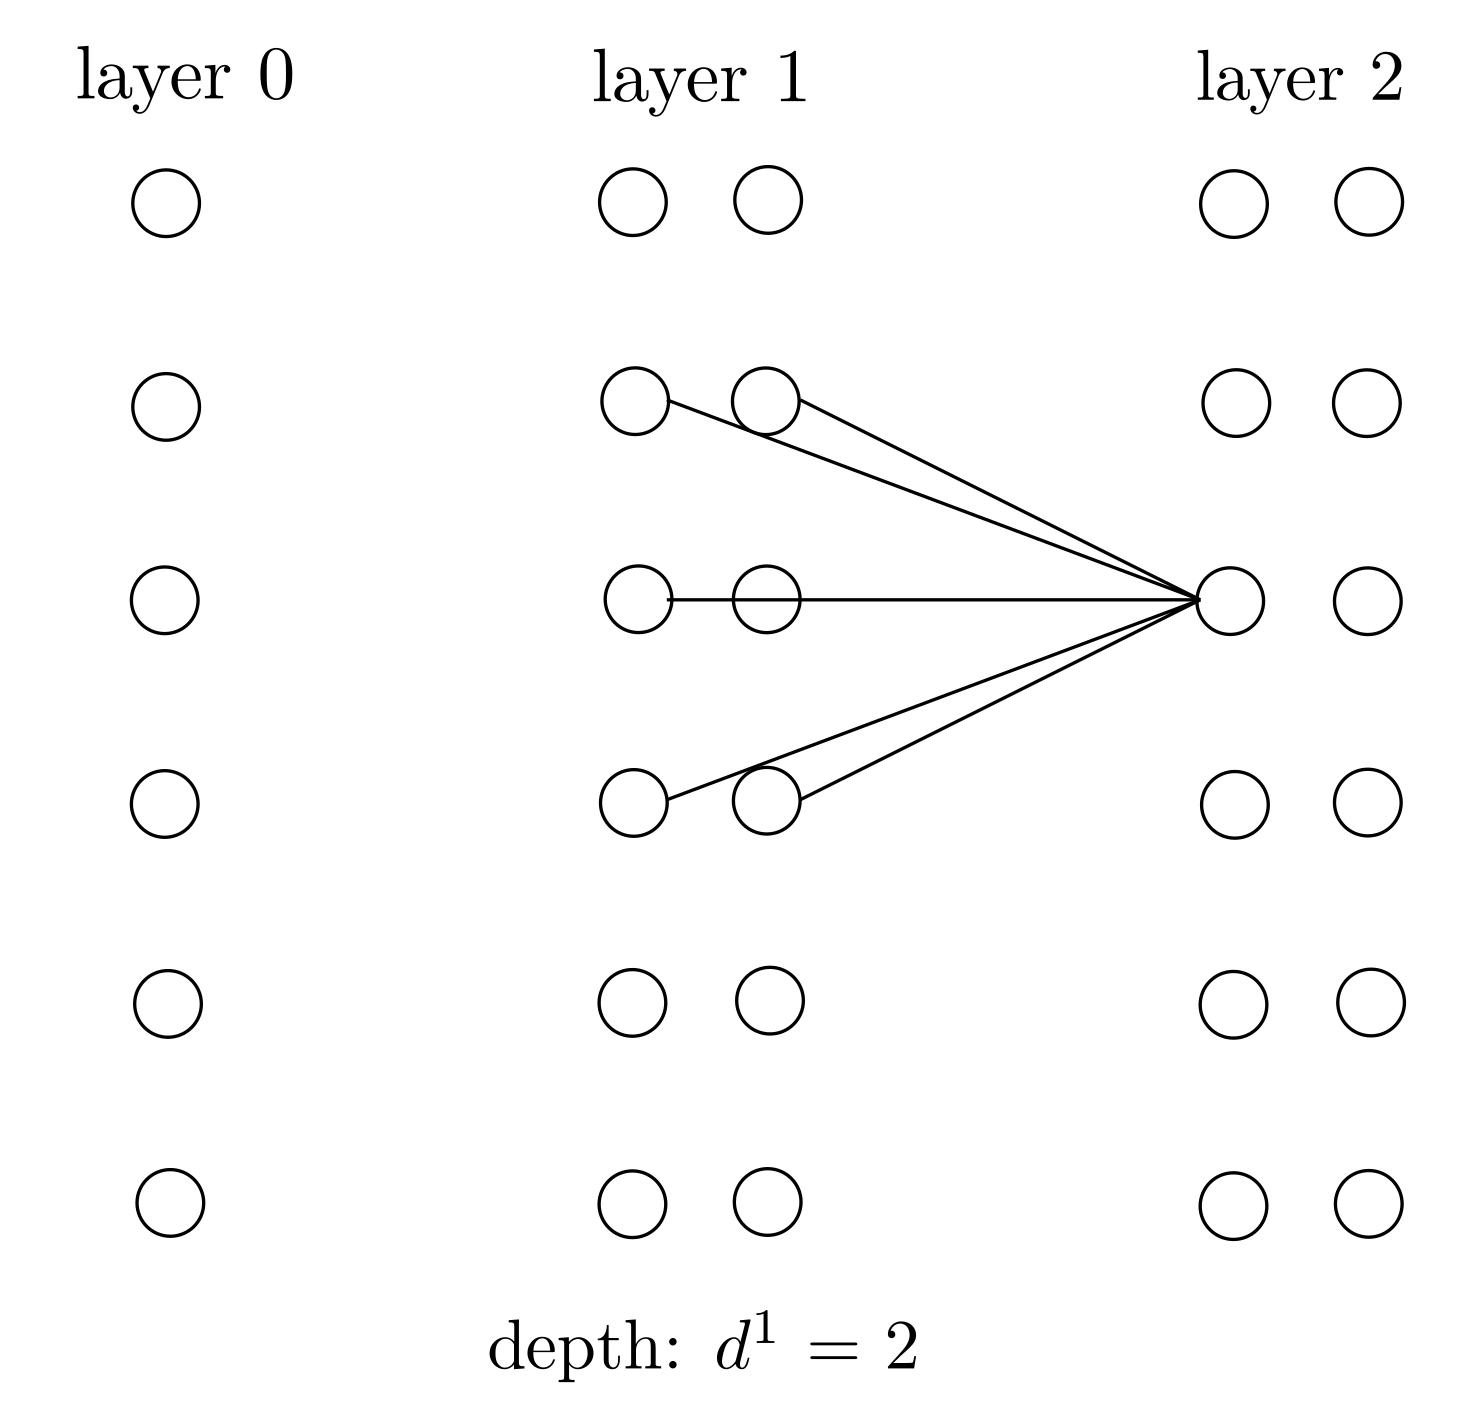
\includegraphics[width=0.53\textwidth]{convolutional_layer3.png}

  \end{center}


}

%%%%%%%%%%%%%%%%%%%%%%%%%%%%%%%%%%%%%%%%%%%%%%%%%%
\frame{
  \frametitle{Several filters in the same convolutional layer}

  \begin{center}
    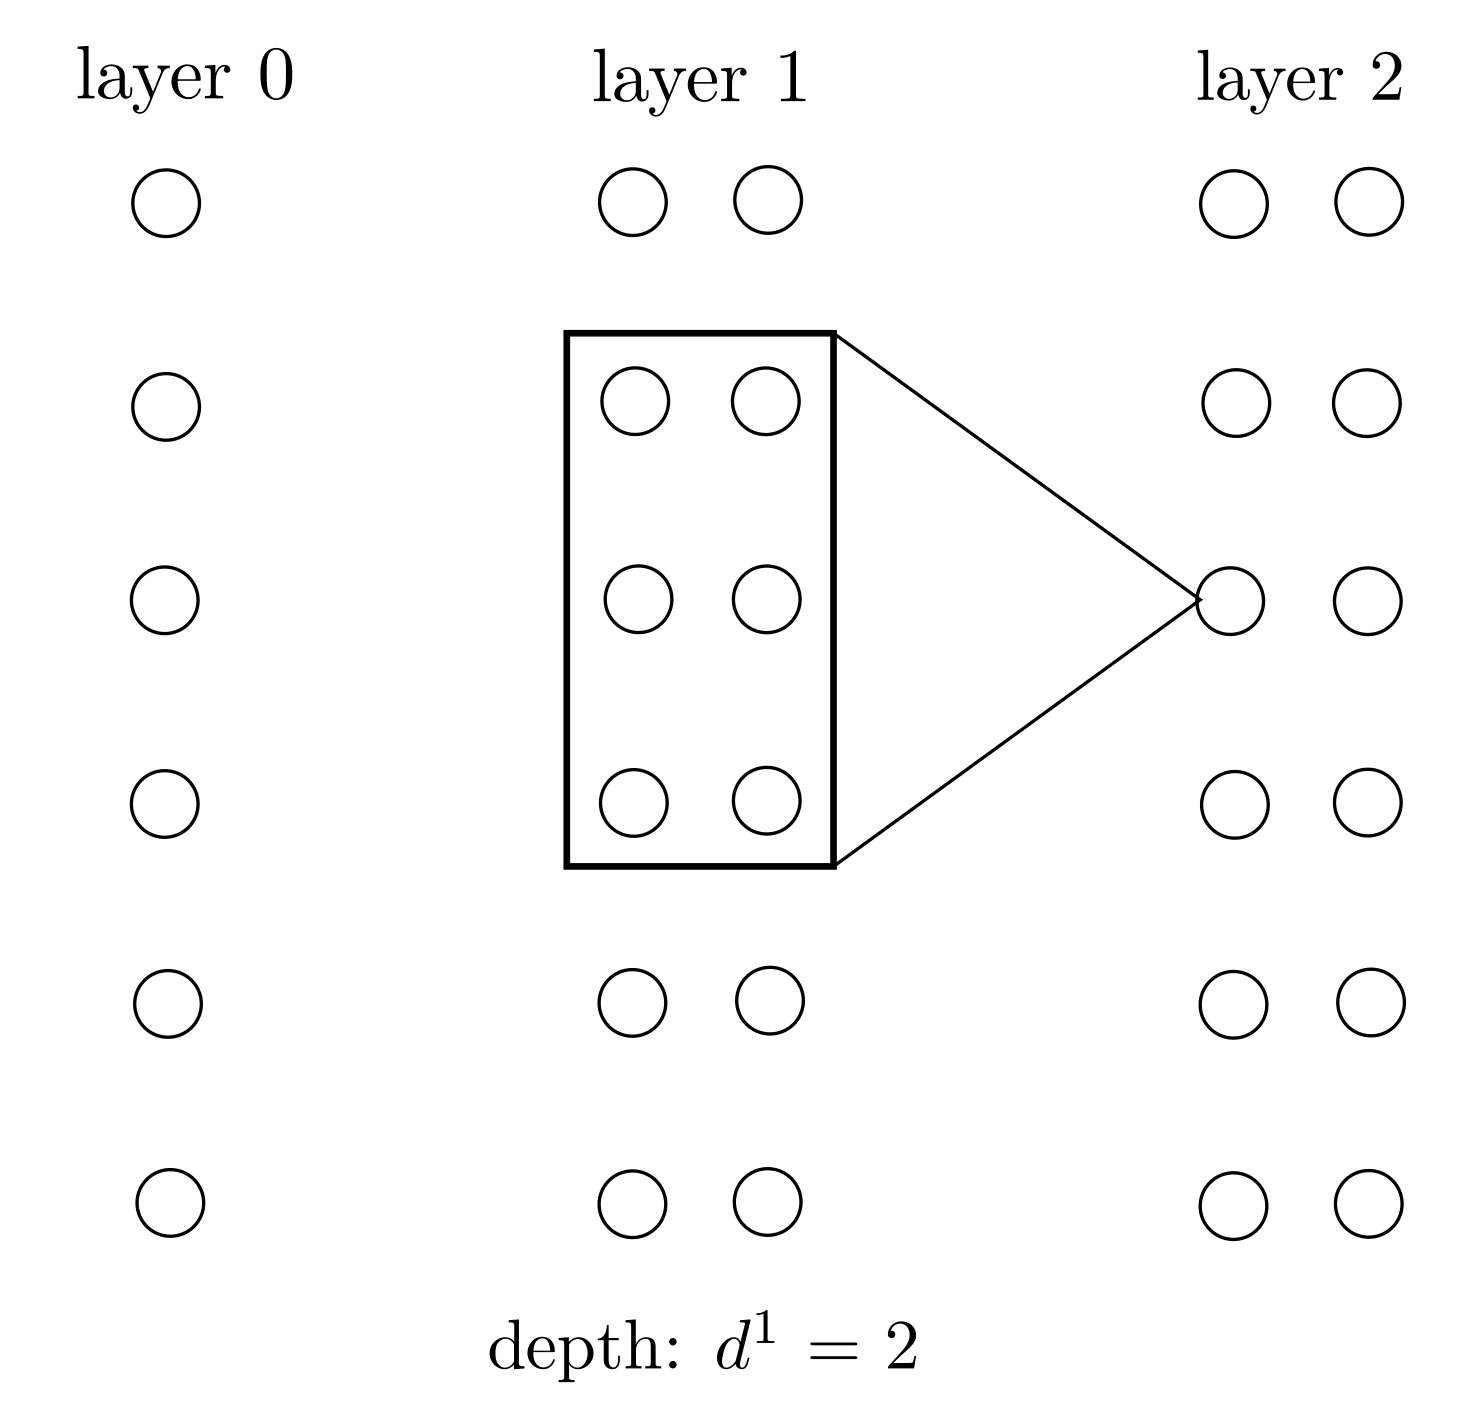
\includegraphics[width=0.53\textwidth]{convolutional_layer4.png}

  \end{center}


}

%%%%%%%%%%%%%%%%%%%%%%%%%%%%%%%%%%%%
\begin{frame}{Branch merging: concatenation}

  \begin{center}
    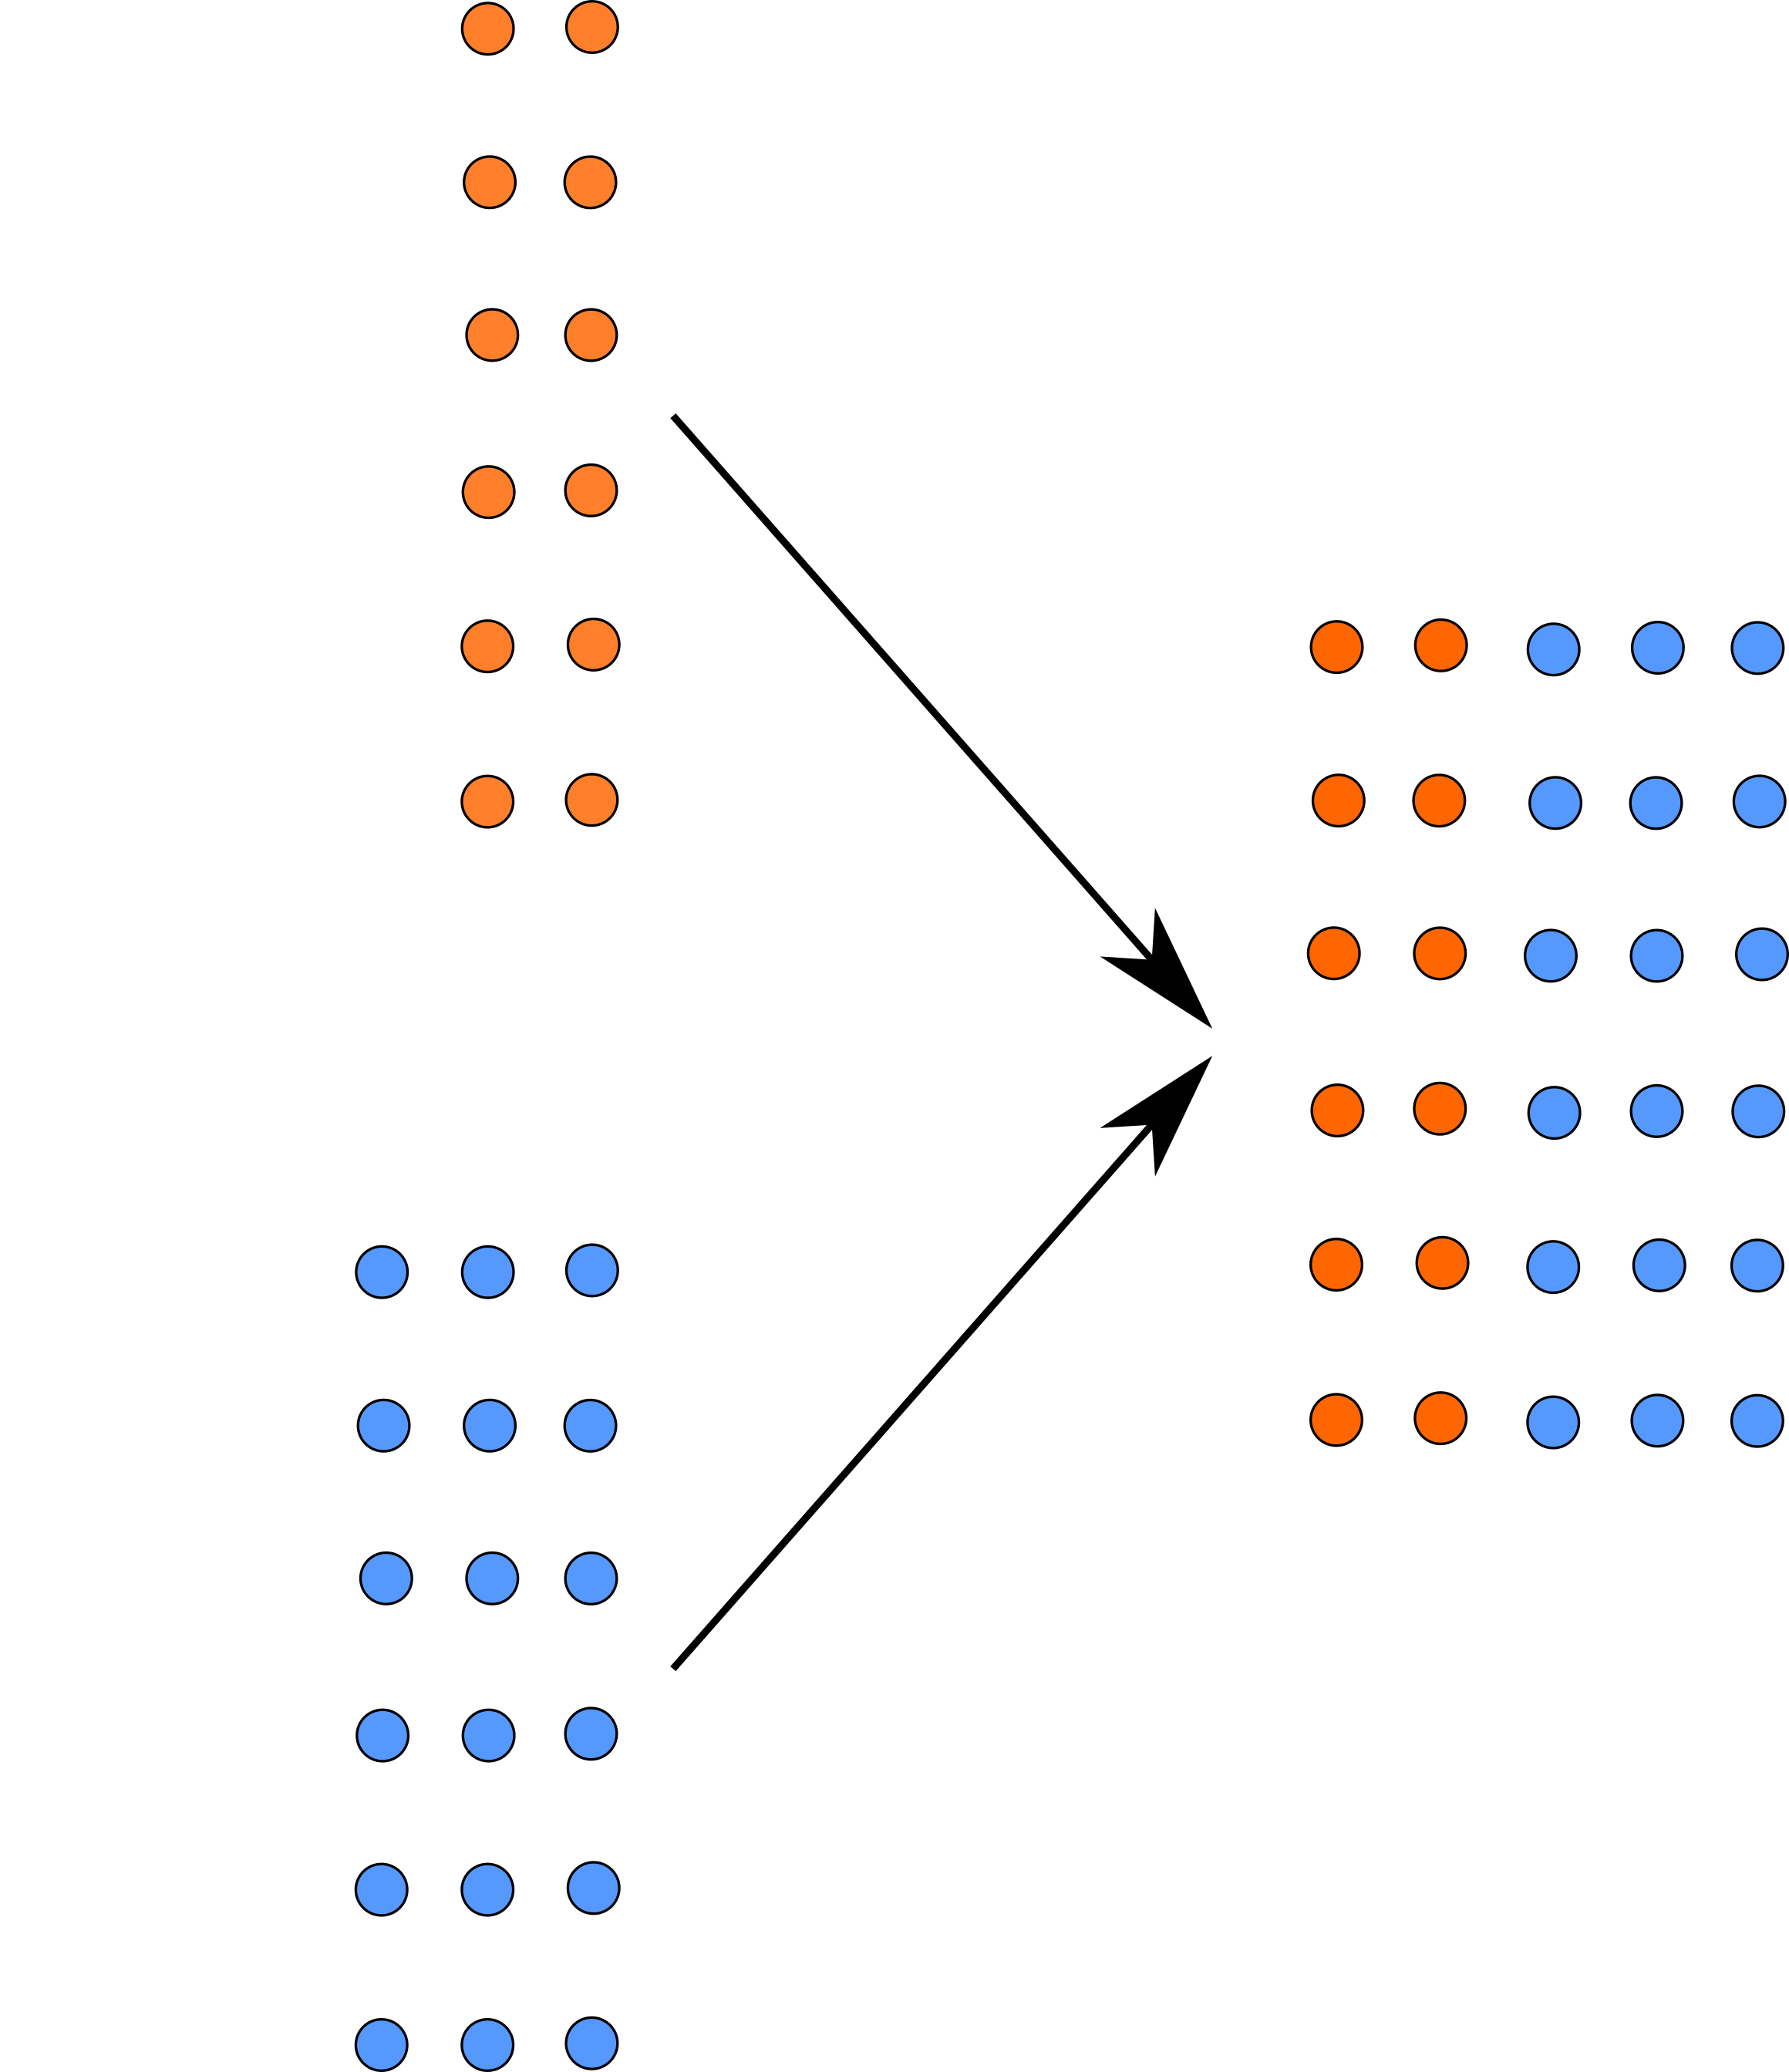
\includegraphics[width=0.5\textwidth]{concatenation.png}
  \end{center}

\end{frame}


%%%%%%%%%%%%%%%%%%%%%%%%%%%%%%%%%%%%
\begin{frame}{1D representations}

  \centering
  \includegraphics[width=\textwidth]{fovea_convnet2}

  \vspace{1em}
  \pause

  \begin{columns}
    \begin{column}{.5\textwidth}
      \includegraphics[width=0.8\textwidth]{Fundus_photograph_of_normal_right_eye.jpg}
    \end{column}
    \begin{column}{.5\textwidth}
      This NN was used to estimate the position of the center of the macula on fundus images.
    \end{column}
  \end{columns}

  \source{NN is work of Robin Alais et al.\\Fundus image by Mikael Häggström, used with permission (CC0).}


\end{frame}

%%%%%%%%%%%%%%%%%%%%%%%%%%%%%%%%%%%%
\begin{frame}{2D representations}

  \begin{center}
    \begin{figure}
      \includegraphics[width=0.75\textwidth]{vgg16.png}
      \source{VGG16 (From https://www.cs.toronto.edu/~frossard/post/vgg16/)}
    \end{figure}
  \end{center}

\end{frame}

%%%%%%%%%%%%%%%%%%%%%%%%%%%%%%%%%%%%
\section{From classification to image-to-image translation}




%%%%%%%%%%%%%%%%%%%%%%%%%%%%%%%%%%%%
%% \begin{frame}{VGG16: a network for image classification}

%%   \begin{center}
%%     \begin{figure}
%%       \centering
%%       \includegraphics[width=0.65\textwidth]{vgg16.png}
%%       \source{VGG16 (From https://www.cs.toronto.edu/~frossard/post/vgg16/)}
%%     \end{figure}
%%   \end{center}


%% \end{frame}



%%%%%%%%%%%%%%%%%%%%%%%%%%%%%%%%%%%%
\begin{frame}{From classification nets to image-to-image nets}

      \begin{figure}
      \includegraphics[width=0.5\textwidth]{image_classif.png}
      \end{figure}

      \pause

      \begin{figure}
      \includegraphics[width=0.5\textwidth]{image_transf.png}
      \end{figure}


\end{frame}


%%%%%%%%%%%%%%%%%%%%%%%%%%%%%%%%%%%%
\begin{frame}{From classification nets to image-to-image nets}

      \begin{figure}
      \includegraphics[width=0.5\textwidth]{image_transf1.png}
      \end{figure}

      \pause

      \begin{figure}
      \includegraphics[width=0.5\textwidth]{image_transf2.png}
      \end{figure}

\end{frame}

%%%%%%%%%%%%%%%%%%%%%%%%%%%%%%%%%%%%
\begin{frame}{From classification nets to image-to-image nets}

      \begin{figure}
      \includegraphics[width=0.5\textwidth]{image_transf_fin.png}
      \end{figure}

\pause

      \begin{itemize}
      \item The neuron membrane segmentation challenge winner~\cite{ciresan_deep_2012} used this strategy. It is inefficient.
      \item The idea to compute the whole output image with a single pass through the network had already been proposed \cite{feng_ning_toward_2005, jain_supervised_2007} (but with architectures more complex than those used today).
      \end{itemize}

\end{frame}


%%%%%%%%%%%%%%%%%%%%%%%%%%%%%%%%%%%%%%%%%%%%%%%%%%
\frame{
  \frametitle{The simplest image-to-image architecture}

  \begin{block}{Example: plain CNN \cite{pang_cell_2010}}
    \begin{figure}
      \includegraphics[width=0.9\textwidth]{plain_convnet.png}
    \end{figure}
  \end{block}

  \pause

Note that today we would use ReLU activations on all layers except the last.

}

%%%%%%%%%%%%%%%%%%%%%%%%%%%%%%%%%%%%
\begin{frame}<beamer>{Going back to the original image size}

    \begin{figure}
      \includegraphics[width=\textwidth]{going_back1.png}
    \end{figure}

\end{frame}


%%%%%%%%%%%%%%%%%%%%%%%%%%%%%%%%%%%%
\begin{frame}<beamer>{Going back to the original image size}

    \begin{figure}
      \includegraphics[width=\textwidth]{going_back2.png}
    \end{figure}

\end{frame}


%%%%%%%%%%%%%%%%%%%%%%%%%%%%%%%%%%%%
\begin{frame}{Going back to the original image size}

    \begin{figure}
      \includegraphics[width=\textwidth]{going_back.png}
    \end{figure}

\end{frame}


%%%%%%%%%%%%%%%%%%%%%%%%%%%%%%%%%%%%
\begin{frame}{Upsampling techniques}


\begin{itemize}
\item Replication
\item Transposed convolution
\item Pooling index memorization
\end{itemize}

\end{frame}

%%%%%%%%%%%%%%%%%%%%%%%%%%%%%%%%%%%%
\begin{frame}{Upsampling through replication}

  \begin{figure}
      \includegraphics[height=0.8\textheight]{upsampling.png}
    \end{figure}

\end{frame}


%%%%%%%%%%%%%%%%%%%%%%%%%%%%%%%%%%%%
\begin{frame}{Transposed convolution}

  \begin{columns}

    \begin{column}<1->{0.3\textwidth}
      \begin{center}
        \includegraphics[width=0.74\textwidth]{convolutional_layer}
        \\ \scriptsize{Convolutional layer}
      \end{center}
    \end{column}

    \begin{column}<2->{0.3\textwidth}
      \begin{center}
        \includegraphics[width=0.74\textwidth]{transposed_conv.png}
        \\ \scriptsize{Transposed convolutional layer}
      \end{center}
    \end{column}

    \begin{column}<3->{0.3\textwidth}
      \begin{center}
        \includegraphics[width=0.74\textwidth]{transposed_conv_stride.png}
        \\ \scriptsize{Transposed convolutional layer with stride $=2$}
      \end{center}
    \end{column}

  \end{columns}


\end{frame}


%%%%%%%%%%%%%%%%%%%%%%%%%%%%%%%%%%%%%%%%%%%%%%%%%%%%%
\section[Properties]{Properties of fully-convolutional neural networks}

%%%%%%%%%%%%%%%%%%%%%%%%%%%%%%%%%%%%%%%%%%%%%%%%%%%%%
\subsection{Receptive field}
%%%%%%%%%%%%%%%%%%%%%%%%%%%%%%%%%%%%%%%%%%%%%%%%%%
\frame{
  \frametitle{Receptive field}

  \begin{block}{Definition: links between neurons}
    In a NN, we say that neuron $a$ is linked to neuron $b$ if there is an oriented path in the corresponding graph going from $a$ to $b$.
  \end{block}


  \begin{block}{Definition}
    The \alert{receptive field} of a neuron in a NN is the set of \emph{input neurons} that are linked to that neuron.

    The size of the receptive field is an essential property when designing a fully-convolutional NN architecture.
  \end{block}

Note that in most cases, receptive fields are square shaped (border effects ignored).

}

%%%%%%%%%%%%%%%%%%%%%%%%%%%%%%%%%%%%
\begin{frame}<beamer>{Illustration}

  \begin{figure}
    \includegraphics[width=0.8\textwidth]{receptive_field.png}
  \end{figure}

\end{frame}

%%%%%%%%%%%%%%%%%%%%%%%%%%%%%%%%%%%%
\begin{frame}<beamer>{Illustration}

  \begin{figure}
  \includegraphics[width=0.8\textwidth]{receptive_field2.png}
  \end{figure}

\end{frame}

%%%%%%%%%%%%%%%%%%%%%%%%%%%%%%%%%%%%
\begin{frame}{Illustration}

  \begin{figure}
  \includegraphics[width=0.8\textwidth]{receptive_field3.png}
  \end{figure}

\end{frame}


%%%%%%%%%%%%%%%%%%%%%%%%%%%%%%%%%%%%%%%%%%%%%%%%%%
\frame{
  \frametitle{Example}

  \begin{block}{}
    \begin{figure}
      \includegraphics[width=0.8\textwidth]{plain_convnet.png}
    \end{figure}
  \end{block}


  \begin{quizzblock}{What is the width of the receptive field of the neurons in the last layer?}
    \begin{enumerate}
    \item $n$
    \item $1 + 2 \times n$
    \item $1 + 2 \times (n+1)$
    \item It depends on the input image
    \end{enumerate}

  \end{quizzblock}

  \mode<beamer>{
  \pause

  Answer: $1 + 2 \times (n+1)$
  }
  }

%%%%%%%%%%%%%%%%%%%%%%%%%%%%%%%%%%%%
\begin{frame}{Conclusion on the receptive field}

  When choosing or designing a NN architecture:
\begin{itemize}
\item Establish its minimal required size with respect to the application
\item Make it larger than that...
\end{itemize}

\end{frame}


%%%%%%%%%%%%%%%%%%%%%%%%%%%%%%%%%%%%%%%%%%%%%%%%%%%%%
\subsection{Translation equivariance}

%%%%%%%%%%%%%%%%%%%%%%%%%%%%%%%%%%%%
\begin{frame}{Equivariance}

\begin{block}{Definition}
  A function $f: E \longrightarrow F$ is \alert{equivariant} with respect to the functions $t_E: E \longrightarrow E$ and $t_F: F \longrightarrow F$ iff $\forall x \in E$:
  \[
  f(t_E(x)) = t_F(f(x))
  \]
\end{block}

\end{frame}

%%%%%%%%%%%%%%%%%%%%%%%%%%%%%%%%%%%%
\begin{frame}{Translation equivariance}

\begin{itemize}
  \item When $E=F$ and $t_E$ and $t_F$ are the same, any, translation, then we have \emph{translation equivariance}.
\item Translation equivariance is an often sought property for image processing operators.
\item Note that we often abusively say \emph{invariant} to translation instead of \emph{equivariant} to translation.
\item Given that in all practical cases images are defined on a bounded set, this property is only true ``far enough'' from the borders
\end{itemize}

\end{frame}




%%%%%%%%%%%%%%%%%%%%%%%%%%%%%%%%%%%%
\begin{frame}{Translation equivariance: comments}

  %% \begin{block}{}
  %%   Identical receptive fields produce identical outputs.
  %% \end{block}

  %% \pause

  \begin{itemize}[<+->]
  \item If padding is used in the network, border effects can be important.
  \item Translation equivariance is not always welcome!
  \item Position information can also be used in the network:
    \begin{itemize}
    \item Through masks or segmentations
    \item Through pixel coordinates
    \end{itemize}
  \end{itemize}

\end{frame}

%%%%%%%%%%%%%%%%%%%%%%%%%%%%%%%%%%%%
\begin{frame}{Illustration}

\begin{figure}[ht]
  \centering
  \includegraphics[height=0.65\textheight]{fundus1}\\
  When aiming to segment the papilla or the macula, translation equivariance is not necessarily welcome.
  \source{OPHDIAT database}
\end{figure}

\end{frame}


%%%%%%%%%%%%%%%%%%%%%%%%%%%%%%%%%%%%%%%%%%%%%%%%%%%%%
\subsection{Other properties}
%%%%%%%%%%%%%%%%%%%%%%%%%%%%%%%%%%%%%%%%%%%%%%%%%%%%%
\frame{
  \frametitle{Image size flexibility}

  \begin{itemize}[<+->]
  \item A NN containing fully-connected layers can only process images of a given size.
  \item \alert{A fully convolutional NN can be applied to images of any size, as long as its dimensions are compatible with the subsampling steps of the network.}
  \item Practical limit: the memory of the system.
  \item Note that as the input image gets larger, border effects become proportionally less present.
  \end{itemize}

}

%%%%%%%%%%%%%%%%%%%%%%%%%%%%%%%%%%%%%%%%%%%%%%%%%%%%%
%% \frame{
%%   \frametitle{Robustness with respect to ground-truth errors}

%%   \begin{block}{}
%%     This is more an empirical observation than a mathematical property, but fully-convolutional NNs tend to be robust with respect to errors in the contours position on the ground-truth.
%%   \end{block}


%% }


%%%%%%%%%%%%%%%%%%%%%%%%%%%%%%%%%%%%%%%%%%%%%%%%%%
\section{Image segmentation}

%%%%%%%%%%%%%%%%%%%%%%%%%%%%%%%%%%%%%%%%%%%%%%%%%%
\frame{
  \frametitle{The specific case of image segmentation}

  \begin{block}{Definition: image segmentation}
    Let $I$ be an image defined on $D$. A segmentation of $I$ is a partition of $D$. In practice the regions of the segmentation should correspond to the objects in $I$, which is application dependant.
  \end{block}


  \begin{itemize}

  \item A partition is often represented as a labelled image

  \item In order to make the segments symmetric, each one is represented by a different channel

  \end{itemize}

  \begin{block}{Image segmentation example}
    \begin{figure}
      \centering
      \includegraphics[height=2.5cm]{pascal_moto}
      \hspace{1em}
      \includegraphics[height=2.5cm]{pascal_moto_seg}\\
      \source{Pascal VOC database}
    \end{figure}
  \end{block}

}

%%%%%%%%%%%%%%%%%%%%%%%%%%%%%%%%%%%%%%%%%%%%%%%%%%
\frame{
  \frametitle{Some vocabulary on segmentation}

  \begin{itemize}

  \item \textbf{Object detection / localization}: bounding box around the object(s).
  \item \textbf{Binary segmentation}: segmentation in 2 classes, background and object.
  \item \textbf{Semantic segmentation}: a label is given to each pixel, according to the object it belongs to.
  \item \textbf{Instance segmentation}: identify each separate object, even if they belong to the same class.

  \end{itemize}

}
%%%%%%%%%%%%%%%%%%%%%%%%%%%%%%%%%%%%%%%%%%%%%%%%%%
% \section{Image segmentation}
%%%%%%%%%%%%%%%%%%%%%%%%%%%%%%%%%%%%%%%%%%%%%%%%%%
\subsection{Binary segmentation}

%%%%%%%%%%%%%%%%%%%%%%%%%%%%%%%%%%%%%%%%%%%%%%%%%%%%%
\frame{
  \frametitle{Neuron membrane segmentation challenge (ISBI 2012)}

  \begin{itemize}
  \item Train: single stack of size $30\times512\times512$.
  \item Test: a second stack of same size.
  \end{itemize}

  \begin{figure}
    \includegraphics[width=9cm]{em_challenge}
  \end{figure}

}

%%%%%%%%%%%%%%%%%%%%%%%%%%%%%%%%%%%%%%%%%%%%%%%%%%%%%
\frame{
  \frametitle{Neuron membrane segmentation challenge winner~\cite{ciresan_deep_2012}}

  \begin{figure}
    \includegraphics[width=9cm]{dnn_ciresan}
  \end{figure}

}

%%%%%%%%%%%%%%%%%%%%%%%%%%%%%%%%%%%%%%%%%%%%%%%%%%
%%%%%%%%%%%%%%%%%%%%%%%%%%%%%%%%%%%%%%%%%%%%%%%%%%
\subsection{Semantic segmentation}


%%%%%%%%%%%%%%%%%%%%%%%%%%%%%%%%%%%%%%%%%%%%%%%%%%%%%
\frame{
  \frametitle{Pascal visual object classes segmentation challenge 2012 \cite{everingham_pascal_2014}}

  \begin{itemize}
  \item 1464 training and 1449 validation images
  \item automatic online test, with unknown images
  \item 20 image categories (cat, sofa, motorbike, person, etc.)
  \end{itemize}

  \begin{figure}
    \includegraphics[height=2.5cm]{pascal_cat}
    \includegraphics[height=2.5cm]{pascal_cat_seg}\\
    \includegraphics[height=2.5cm]{pascal_moto}
    \includegraphics[height=2.5cm]{pascal_moto_seg}
  \end{figure}

}

%%%%%%%%%%%%%%%%%%%%%%%%%%%%%%%%%%%%%%%%%%%%%%%%%%%%%

\frame{
  \frametitle{Convolutional nets for semantic image segmentation}

  Three papers in 2015:

  \begin{itemize}

  \item Fully convolutional networks for semantic segmentation \cite{long_fully_2015}
  \item U-Net: convolutional networks for biomedical image segmentation \cite{ronneberger_u-net:_2015}
  \item SegNet: A Deep Convolutional Encoder-Decoder Architecture for Image Segmentation \cite{badrinarayanan_segnet:_2015}

  \end{itemize}

}

%% %%%%%%%%%%%%%%%%%%%%%%%%%%%%%%%%%%%%%%%%%%%%%%%%%%
%% \frame{
%%   \frametitle{Example: U-Net architecture \cite{ronneberger_u-net:_2015}}

%%   \begin{figure}
%%     \includegraphics[height=7cm]{unet}
%%   \end{figure}
%% }



%%%%%%%%%%%%%%%%%%%%%%%%%%%%%%%%%%%%%%%%%%%%%%%%%%
%% \frame{
%%   \frametitle{Example: SegNet architecture \cite{badrinarayanan_segnet:_2015}}

%%   \begin{figure}
%%     \includegraphics[width=9cm]{segnet_archi}
%%   \end{figure}
%% }

%%%%%%%%%%%%%%%%%%%%%%%%%%%%%%%%%%%%%%%%%%%%%%%%%%

\frame{
  \frametitle{Remarks}

  \begin{itemize}
  \item These architectures easily contain a number of parameters of the order of $10^7$ (28 million for U-Net)
  \item Their optimization might be difficult
  \item But you can reduce the number of filters or the number of layers

  \end{itemize}

}

%%%%%%%%%%%%%%%%%%%%%%%%%%%%%%%%%%%%%%%%%%%%%%%%%%%%%
%%%%%%%%%%%%%%%%%%%%%%%%%%%%%%%%%%%%%%%%%%%%%%%%%%%%%
\subsection{Instance segmentation}
%%%%%%%%%%%%%%%%%%%%%%%%%%%%%%%%%%%%%%%%%%%%%%%%%%

\frame{
  \frametitle{COCO: common objects in context \cite{lin_microsoft_2014}}

  \begin{itemize}
  \item $2$ million objects, from $80$ categories, in $300\,000$ images
  \end{itemize}


  \begin{figure}
    \includegraphics[height=3.4cm]{coco_ex_horses}
    \includegraphics[height=3.4cm]{coco_ex_salle_de_bain}
  \end{figure}

  \begin{block}{}
    Winner 2016: Fully Convolutional Instance-aware Semantic Segmentation (Microsoft) \cite{li_fully_2016}
  \end{block}

}


%%%%%%%%%%%%%%%%%%%%%%%%%%%%%%%%%%%%%%%%%%%%%%%%%%%%%
\frame{
  \frametitle{COCO instance segmentation challenge: examples of 2016 winner results}

  \begin{figure}
    \includegraphics[width=4.5cm]{COCO_test2015_000000003241.png}
    \hspace{1cm}
    \includegraphics[width=4.5cm]{COCO_test2015_000000004178.png}\\
    \includegraphics[width=4.5cm]{COCO_test2015_000000006147.png}
    \hspace{1cm}
    \includegraphics[width=4.5cm]{COCO_test2015_000000016177.png}
  \end{figure}

}


%%%%%%%%%%%%%%%%%%%%%%%%%%%%%%%%%%%%%%%%%%%%%%%%%%%%%
%% \frame{
%%   \frametitle{Partially supervised segmentation - \cite{hu_learning_2017}}

%%   \begin{itemize}
%%   \item 80 segmented categories from COCO database (320k images)
%%   \item 3000 visual concepts using box annotations from the Visual Genome data set (100k images)
%%   \end{itemize}

%%   \begin{figure}
%%     \includegraphics[width=12cm]{segm_every_thing_method.png}
%%   \end{figure}

%% }

%%%%%%%%%%%%%%%%%%%%%%%%%%%%%%%%%%%%%%%%%%%%%%%%%%%%%
%% \frame{
%%   \frametitle{Partially supervised segmentation - learning to segment every thing}

%%   \begin{figure}
%%     \includegraphics[width=8cm]{segment_every_thing.png}
%%   \end{figure}

%% \cite{hu_learning_2017}

%%   }

%%%%%%%%%%%%%%%%%%%%%%%%%%%%%%%%%%%%%%%%%%%%%%%%%%
%% \frame{
%%   \frametitle{Current (?) trends for instance segmentation}

%%   \begin{itemize}

%%   \item Region proposal +
%%   \item Fully convolutional (very deep) network +
%%   \item (Post-processing)

%%   \end{itemize}

%%   \begin{figure}
%%     \includegraphics[width=9.5cm]{r_cnn.png}
%%     \caption{Regions with CNN features (R-CNN) (from \cite{girshick_rich_2014})}
%%   \end{figure}

%%   \begin{block}<2->{Meanwhile, on the object detection field...}
%%     \begin{itemize}
%%     \item YOLO: you look only once \cite{redmon_yolo9000:_2016}
%%     \item SSD: single shot detector \cite{liu_ssd:_2016}
%%     \end{itemize}
%%   \end{block}

%% }

%%%%%%%%%%%%%%%%%%%%%%%%%%%%%%%%%%%%%%%%%%%%%%%%%%

%% \frame{
%% \frametitle{A typical convolutional architecture for image classification}

%% \begin{figure}
%%   \includegraphics[width=9.5cm]{conv_net_classif}
%%   \caption{Architecture used for the classification of the NORB dataset (from \cite{scherer_evaluation_2010})}
%% \end{figure}

%% Note that layer P4 can be seen as made of features, which are then classified by the two fully connected layers.


%% }


%%%%%%%%%%%%%%%%%%%%%%%%%%%%%%%%%%%%%%%%%%%%%%%%%%
\subsection{U-Net}

%%%%%%%%%%%%%%%%%%%%%%%%%%%%%%%%%%%%%%%%%%%%%%%%%%
\frame{
  \frametitle{U-Net architecture \cite{ronneberger_u-net:_2015}}

  \begin{figure}
    \includegraphics[width=0.95\textwidth]{unet_lo}
  \end{figure}

  \begin{quizzblock}{Quizz}
  \begin{itemize}
  \item Size and number of channels of input images?
  \item Segmentation into how many regions?
  \end{itemize}
  \end{quizzblock}

}

%%%%%%%%%%%%%%%%%%%%%%%%%%%%%%%%%%%%
\begin{frame}{U-Net main ideas}

      \begin{figure}
        \includegraphics[width=0.86\textwidth]{unet_lo}
      \end{figure}


      \begin{itemize}
      \item Encoding branch inspired by classification nets
      \item Decoding branch is symmetrical
      \item Skip connections
      \end{itemize}

\end{frame}

%%%%%%%%%%%%%%%%%%%%%%%%%%%%%%%%%%%%%%%%%%%%%%%%%%
%% \frame{
%%   \frametitle{U-Net details}

%%   \begin{columns}
%%     \begin{column}{.4\textwidth}
%%       \begin{figure}
%%         \includegraphics[width=\textwidth]{unet_lo}
%%       \end{figure}

%%     \end{column}

%%     \begin{column}{.6\textwidth}

%%       \begin{itemize}
%%       \item Activation of the last layer: soft-max
%%       \item Other activations: ReLU
%%       \item Loss used in the original publication: cross entropy with a weight map $w$ to favor some pixels:
%%         \[
%%         L(\param) = \sum\limits_{M \in D} w(M)\log(\hat{y}_{l(M)}(M))
%%         \]
%%       \end{itemize}

%%     \end{column}
%%   \end{columns}

%% }

%%%%%%%%%%%%%%%%%%%%%%%%%%%%%%%%%%%%
%% \begin{frame}{Illustration}

%% \end{frame}


%%%%%%%%%%%%%%%%%%%%%%%%%%%%%%%%%%%%
\begin{frame}{U-Net improvements}

  \begin{itemize}
  \item Convolutions with stride 2 instead of max-pooling in the encoder
  \item Transposed convolutions instead  of simple up-sampling in the decoder
  \item Batch normalization
  \item Using an already optimized classification network as backbone for the encoder
  \end{itemize}

\end{frame}



%% %%%%%%%%%%%%%%%%%%%%%%%%%%%%%%%%%%%%%%%%%%%%%%%%%%
%% \section[Using CNNs]{Using fully-convolutional networks}

%%%%%%%%%%%%%%%%%%%%%%%%%%%%%%%%%%%%
\begin{frame}{Dealing with image sizes during training}

  \begin{itemize}[<+->]
  \item   In segmentation applications, original images are often of different sizes and possibly very large.
  \item   In theory, given the translation equivariance of fully-convolutional NN, we could use them directly as input. In practice, we are limited by memory size.
  \item   Solution: extract fixed-sized crops from your training set:
    \begin{itemize}
    \item make them as large as possible, to reduce border effects
    \end{itemize}

  \end{itemize}

\end{frame}


%%%%%%%%%%%%%%%%%%%%%%%%%%%%%%%%%%%%%%%%%%%%%%%%%%%%%
%% \frame{
%%   \frametitle{Post-processing for segmentation}

%%   \begin {itemize}
%%   \item Superpixels (e.g. \cite{farabet_learning_2013})
%%   \item Conditional random fields
%%   \item Mathematical morphology
%%   \end{itemize}

%% }


%%%%%%%%%%%%%%%%%%%%%%%%%%%%%%%%%%%%%%%%%%%%%%%%%%
\frame{
  \frametitle{Loss functions for image segmentation}


  \begin{itemize}
  \item $\hat{\y} = (\hat{\y}_i)$: network output
  \item $\y = (\y_i)$: binary expected output
  \item We suppose that all $\hat{\y}_i$ are in $[0,1]$
  \item We want the $\hat{\y}$ to be \emph{as close as possible} to $\y$
  \end{itemize}

}


%%%%%%%%%%%%%%%%%%%%%%%%%%%%%%%%%%%%%%%%%%%%%%%%%%
\frame{
  \frametitle{Loss functions for image segmentation}


  \begin{block}{A loss function inherited from image classification}

    \begin{itemize}
    \item Cross-entropy: $ -\sum\limits_i y_i\log(\hat{y}_i)$
    \end{itemize}

  \end{block}

}

%%%%%%%%%%%%%%%%%%%%%%%%%%%%%%%%%%%%%%%%%%%%%%%%%%
\frame{
  \frametitle{Measures used in image processing}

  Let $A$ and $B$ be two sets, not simultaneously empty.

  \begin{columns}
    \begin{column}{.7\textwidth}
      \begin{block}{Dice coefficient}
        \[
        D(A,B) = \frac{2|A \cap B|}{|A|+|B|}
        \]
      \end{block}

      \begin{block}{Jaccard index}
        \[
        J(A,B) = \frac{|A \cap B|}{|A \cup B|}
        \]
      \end{block}


    \end{column}

    \begin{column}{.3\textwidth}
      \includegraphics[width=\textwidth]{Intersection_of_sets_A_and_B}
      \source{Public domain (Wikipedia.org)}
    \end{column}
  \end{columns}


  \begin{block}{Properties}
    \begin{itemize}
    \item $\forall A, B: 0 \leq J(A, B) \leq D(A,B) \leq 1$
    \item If $A=B$, then $D(A,B) = J(A,B) = 1$
    \item If $ A \cap B = \emptyset$, then $D(A,B) = J(A,B) = 0$
    \end{itemize}
  \end{block}

}


%%%%%%%%%%%%%%%%%%%%%%%%%%%%%%%%%%%%%%%%%%%%%%%%%%
\frame{
  \frametitle{Generalization to $[0,1]$}

      \begin{block}{Jaccard index}
        \[
        J(A,B) = \frac{|A \cap B|}{|A \cup B|}
        \]
      \end{block}

      But $\y$ and $\hat{\y}$ are in $[0,1]^n \ldots$

\pause

  %% \begin{block}{Dice similarity}
  %%   \[
  %%   D(\y, \hat{\y}) = \frac{2\sum_i y_i\hat{y}_i}{\sum_i y_i + \sum_i \hat{y}_i}
  %%   \]
  %% \end{block}

  \begin{block}{Jaccard similarity}
    \[
    J(\y, \hat{\y}) = \frac{\sum_i y_i\hat{y}_i}{\sum_i y_i + \sum_i \hat{y}_i - \sum_i y_i\hat{y}_i}
    \]
  \end{block}

($\y$ and $\hat{\y}$ are not simultaneously equal to $0$)

}


%%%%%%%%%%%%%%%%%%%%%%%%%%%%%%%%%%%%%%%%%%%%%%%%%%
\frame{
  \frametitle{Corresponding loss function}


  %% \begin{block}{Dice loss}
  %%   \[
  %%   d(\y, \hat{\y}) = 1-\frac{2\sum_i y_i\hat{y}_i}{\sum_i y_i + \sum_i \hat{y}_i}
  %%   \]
  %% \end{block}

  \begin{block}{Jaccard loss}
    \[
    j(\y, \hat{\y}) = 1-\frac{\sum_i y_i\hat{y}_i}{\sum_i y_i + \sum_i \hat{y}_i - \sum_i y_i\hat{y}_i + \epsilon}
    \]
  \end{block}

    Constant $\epsilon$, which is typically ``small'', keeps the denominator ``far enough'' from zero.


}

%%%%%%%%%%%%%%%%%%%%%%%%%%%%%%%%%%%%%%%%%%%%%%%%%%
\frame{
  \frametitle{Corresponding loss function - variant}


  %% \begin{block}{Dice loss}
  %%   \[
  %%   d(\y, \hat{\y}) = 1-\frac{2\sum_i y_i\hat{y}_i}{\sum_i y_i^2 + \sum_i \hat{y}_i^2 + \epsilon}
  %%   \]
  %% \end{block}

  \begin{block}{Jaccard loss}
    \[
    j_2(\y, \hat{\y}) = 1-\frac{\sum_i y_i\hat{y}_i}{\sum_i y_i^2 + \sum_i \hat{y}_i^2 - \sum_i y_i\hat{y}_i + \epsilon}
    \]
  \end{block}

This version works slightly better than the first~\cite{duque-arias_power_2021}.

}


%%%%%%%%%%%%%%%%%%%%%%%%%%%%%%%%%%%%
\begin{frame}{Conclusion on loss functions}

  \begin{itemize}
  \item Use the Jaccard loss as base line for segmentation problems.
  \item Note that these losses compute their values pixel-wise: they do not take into account any structure (for example, continuity).
  \item Working on specific losses enforcing structure = interesting research path.
  \end{itemize}
\end{frame}

%%%%%%%%%%%%%%%%%%%%%%%%%%%%%%%%%%%%%%%%%%%%%%%%%%
\section{3D}


%%%%%%%%%%%%%%%%%%%%%%%%%%%%%%%%%%%%
\begin{frame}{Processing 3D images}

\begin{itemize}
\item 2D: Slice by slice
\item 2,5D image: to treat slice $s$, take into account slices $s-1$ and $s+1$
\item 3D
\end{itemize}

\end{frame}

%%%%%%%%%%%%%%%%%%%%%%%%%%%%%%%%%%%%
\begin{frame}{Advantage and drawbacks of 3D approaches}

\begin{block}{Advantage}
  \begin{itemize}
  \item 3D structure
  \end{itemize}
\end{block}

\begin{block}{Drawbacks}
  \begin{itemize}
  \item Memory usage, smaller 2D receptive field
  \item Annotation
  \end{itemize}
\end{block}

\end{frame}

%%%%%%%%%%%%%%%%%%%%%%%%%%%%%%%%%%%%
\begin{frame}{Example~\cite{bertoldo_modular_2021}}

\begin{figure}[ht]
  \centering
  \includegraphics[width=\textwidth]{casagrande_annotations}\\
  Annotated X-CT of polyamide 66 reinforced by glass fibers
\end{figure}

\end{frame}


%%%%%%%%%%%%%%%%%%%%%%%%%%%%%%%%%%%%
\begin{frame}{Quantitative results}

\begin{figure}[ht]
  \centering
  \includegraphics[width=0.9\textwidth]{casagrande_variations}
\end{figure}


\end{frame}

%%%%%%%%%%%%%%%%%%%%%%%%%%%%%%%%%%%%
\begin{frame}{Test}

\begin{figure}[ht]
  \centering
  \includegraphics[width=\textwidth]{casagrande_test}
\end{figure}


\end{frame}



%%%%%%%%%%%%%%%%%%%%%%%%%%%%%%%%%%%%%%%%%%%%%%%%%%
%%%%%%%%%%%%%%%%%%%%%%%%%%%%%%%%%%%%%%%%%%%%%%%%%%
\section{Conclusion}

%%%%%%%%%%%%%%%%%%%%%%%%%%%%%%%%%%%%%%%%%%%%%%%%%%%%%
\frame{
  \frametitle{Image segmentation: a solved problem?}

  \begin {itemize}
  \item Progress in image segmentation since 2012 has been enormous
  \item Several complex problems have now satisfactory solutions
  \item Training can be a problem (large annotated databases, difficult optimization)
  \item There are still challenges ahead...
  \end{itemize}

}

%%%%%%%%%%%%%%%%%%%%%%%%%%%%%%%%%%%%
\begin{frame}{Some research subjects}

  \begin{itemize}
  \item Optimization - a very general, and essential, subject
  \item Making training databases as small as possible
  \item Specific losses
  \item Taking  {\it a priori} structural information into account
  \item Transformers for image segmentation
  \end{itemize}

\end{frame}

%%%%%%%%%%%%%%%%%%%%%%%%%%%%%%%%%%%%
\begin{frame}{IntACT segmentation course material}

\begin{block}{}
  \url{https://colibris.link/RasJ1}
\end{block}

\end{frame}




%%%%%%%%%%%%%%%%%%%%%%%%%%%%%%%%%%%%%%%%%%%%%%%%%%
\section*{References}

%%%%%%%%%%%%%%%%%%%%%%%%%%%%%%%%%%%%%%%%%%%%%%%%%%

\frame[allowframebreaks]{

  \scriptsize

  \frametitle{References}

  %\bibliographystyle{amsalpha}
  %\bibliographystyle{apalike}

  \bibliography{../../edf.bib,slides_deep.bib}

  \normalsize

}



\end{document}

% https://colibris.link/RasJ1
